\documentclass[twoside]{book}

% Packages required by doxygen
\usepackage{fixltx2e}
\usepackage{calc}
\usepackage{doxygen}
\usepackage[export]{adjustbox} % also loads graphicx
\usepackage{graphicx}
\usepackage[utf8]{inputenc}
\usepackage{makeidx}
\usepackage{multicol}
\usepackage{multirow}
\PassOptionsToPackage{warn}{textcomp}
\usepackage{textcomp}
\usepackage[nointegrals]{wasysym}
\usepackage[table]{xcolor}

% Font selection
\usepackage[T1]{fontenc}
\usepackage[scaled=.90]{helvet}
\usepackage{courier}
\usepackage{amssymb}
\usepackage{sectsty}
\renewcommand{\familydefault}{\sfdefault}
\allsectionsfont{%
  \fontseries{bc}\selectfont%
  \color{darkgray}%
}
\renewcommand{\DoxyLabelFont}{%
  \fontseries{bc}\selectfont%
  \color{darkgray}%
}
\newcommand{\+}{\discretionary{\mbox{\scriptsize$\hookleftarrow$}}{}{}}

% Page & text layout
\usepackage{geometry}
\geometry{%
  a4paper,%
  top=2.5cm,%
  bottom=2.5cm,%
  left=2.5cm,%
  right=2.5cm%
}
\tolerance=750
\hfuzz=15pt
\hbadness=750
\setlength{\emergencystretch}{15pt}
\setlength{\parindent}{0cm}
\setlength{\parskip}{3ex plus 2ex minus 2ex}
\makeatletter
\renewcommand{\paragraph}{%
  \@startsection{paragraph}{4}{0ex}{-1.0ex}{1.0ex}{%
    \normalfont\normalsize\bfseries\SS@parafont%
  }%
}
\renewcommand{\subparagraph}{%
  \@startsection{subparagraph}{5}{0ex}{-1.0ex}{1.0ex}{%
    \normalfont\normalsize\bfseries\SS@subparafont%
  }%
}
\makeatother

% Headers & footers
\usepackage{fancyhdr}
\pagestyle{fancyplain}
\fancyhead[LE]{\fancyplain{}{\bfseries\thepage}}
\fancyhead[CE]{\fancyplain{}{}}
\fancyhead[RE]{\fancyplain{}{\bfseries\leftmark}}
\fancyhead[LO]{\fancyplain{}{\bfseries\rightmark}}
\fancyhead[CO]{\fancyplain{}{}}
\fancyhead[RO]{\fancyplain{}{\bfseries\thepage}}
\fancyfoot[LE]{\fancyplain{}{}}
\fancyfoot[CE]{\fancyplain{}{}}
\fancyfoot[RE]{\fancyplain{}{\bfseries\scriptsize Generated by Doxygen }}
\fancyfoot[LO]{\fancyplain{}{\bfseries\scriptsize Generated by Doxygen }}
\fancyfoot[CO]{\fancyplain{}{}}
\fancyfoot[RO]{\fancyplain{}{}}
\renewcommand{\footrulewidth}{0.4pt}
\renewcommand{\chaptermark}[1]{%
  \markboth{#1}{}%
}
\renewcommand{\sectionmark}[1]{%
  \markright{\thesection\ #1}%
}

% Indices & bibliography
\usepackage{natbib}
\usepackage[titles]{tocloft}
\setcounter{tocdepth}{3}
\setcounter{secnumdepth}{5}
\makeindex

% Hyperlinks (required, but should be loaded last)
\usepackage{ifpdf}
\ifpdf
  \usepackage[pdftex,pagebackref=true]{hyperref}
\else
  \usepackage[ps2pdf,pagebackref=true]{hyperref}
\fi
\hypersetup{%
  colorlinks=true,%
  linkcolor=blue,%
  citecolor=blue,%
  unicode%
}

% Custom commands
\newcommand{\clearemptydoublepage}{%
  \newpage{\pagestyle{empty}\cleardoublepage}%
}

\usepackage{caption}
\captionsetup{labelsep=space,justification=centering,font={bf},singlelinecheck=off,skip=4pt,position=top}

%===== C O N T E N T S =====

\begin{document}

% Titlepage & ToC
\hypersetup{pageanchor=false,
             bookmarksnumbered=true,
             pdfencoding=unicode
            }
\pagenumbering{alph}
\begin{titlepage}
\vspace*{7cm}
\begin{center}%
{\Large L\+P\+OO Project }\\
\vspace*{1cm}
{\large Generated by Doxygen 1.8.13}\\
\end{center}
\end{titlepage}
\clearemptydoublepage
\pagenumbering{roman}
\tableofcontents
\clearemptydoublepage
\pagenumbering{arabic}
\hypersetup{pageanchor=true}

%--- Begin generated contents ---
\chapter{Hierarchical Index}
\section{Class Hierarchy}
This inheritance list is sorted roughly, but not completely, alphabetically\+:\begin{DoxyCompactList}
\item \contentsline{section}{dkeep.\+logic.\+Cell\+Position}{\pageref{classdkeep_1_1logic_1_1_cell_position}}{}
\item Serializable\begin{DoxyCompactList}
\item \contentsline{section}{dkeep.\+logic.\+Character}{\pageref{classdkeep_1_1logic_1_1_character}}{}
\begin{DoxyCompactList}
\item \contentsline{section}{dkeep.\+logic.\+Crazy\+Ogre}{\pageref{classdkeep_1_1logic_1_1_crazy_ogre}}{}
\item \contentsline{section}{dkeep.\+logic.\+Guard}{\pageref{classdkeep_1_1logic_1_1_guard}}{}
\begin{DoxyCompactList}
\item \contentsline{section}{dkeep.\+logic.\+Drunken\+Guard}{\pageref{classdkeep_1_1logic_1_1_drunken_guard}}{}
\item \contentsline{section}{dkeep.\+logic.\+Rookie\+Guard}{\pageref{classdkeep_1_1logic_1_1_rookie_guard}}{}
\item \contentsline{section}{dkeep.\+logic.\+Suspicious\+Guard}{\pageref{classdkeep_1_1logic_1_1_suspicious_guard}}{}
\end{DoxyCompactList}
\item \contentsline{section}{dkeep.\+logic.\+Hero}{\pageref{classdkeep_1_1logic_1_1_hero}}{}
\end{DoxyCompactList}
\item \contentsline{section}{dkeep.\+logic.\+Dungeon\+Logic}{\pageref{classdkeep_1_1logic_1_1_dungeon_logic}}{}
\item \contentsline{section}{dkeep.\+logic.\+Dungeon\+Map}{\pageref{classdkeep_1_1logic_1_1_dungeon_map}}{}
\item \contentsline{section}{dkeep.\+logic.\+Game}{\pageref{classdkeep_1_1logic_1_1_game}}{}
\item \contentsline{section}{dkeep.\+logic.\+Guard}{\pageref{classdkeep_1_1logic_1_1_guard}}{}
\item \contentsline{section}{dkeep.\+logic.\+Keep\+Logic}{\pageref{classdkeep_1_1logic_1_1_keep_logic}}{}
\item \contentsline{section}{dkeep.\+logic.\+Keep\+Map}{\pageref{classdkeep_1_1logic_1_1_keep_map}}{}
\item \contentsline{section}{dkeep.\+logic.\+Logic}{\pageref{classdkeep_1_1logic_1_1_logic}}{}
\begin{DoxyCompactList}
\item \contentsline{section}{dkeep.\+logic.\+Dungeon\+Logic}{\pageref{classdkeep_1_1logic_1_1_dungeon_logic}}{}
\item \contentsline{section}{dkeep.\+logic.\+Keep\+Logic}{\pageref{classdkeep_1_1logic_1_1_keep_logic}}{}
\end{DoxyCompactList}
\item \contentsline{section}{dkeep.\+logic.\+Map}{\pageref{classdkeep_1_1logic_1_1_map}}{}
\begin{DoxyCompactList}
\item \contentsline{section}{dkeep.\+logic.\+Dungeon\+Map}{\pageref{classdkeep_1_1logic_1_1_dungeon_map}}{}
\item \contentsline{section}{dkeep.\+logic.\+Keep\+Map}{\pageref{classdkeep_1_1logic_1_1_keep_map}}{}
\end{DoxyCompactList}
\item \contentsline{section}{dkeep.\+logic.\+Weapon}{\pageref{classdkeep_1_1logic_1_1_weapon}}{}
\begin{DoxyCompactList}
\item \contentsline{section}{dkeep.\+logic.\+Club}{\pageref{classdkeep_1_1logic_1_1_club}}{}
\end{DoxyCompactList}
\end{DoxyCompactList}
\end{DoxyCompactList}

\chapter{Class Index}
\section{Class List}
Here are the classes, structs, unions and interfaces with brief descriptions\+:\begin{DoxyCompactList}
\item\contentsline{section}{\hyperlink{classdkeep_1_1logic_1_1_cell_position}{dkeep.\+logic.\+Cell\+Position} }{\pageref{classdkeep_1_1logic_1_1_cell_position}}{}
\item\contentsline{section}{\hyperlink{classdkeep_1_1logic_1_1_character}{dkeep.\+logic.\+Character} }{\pageref{classdkeep_1_1logic_1_1_character}}{}
\item\contentsline{section}{\hyperlink{classdkeep_1_1logic_1_1_club}{dkeep.\+logic.\+Club} }{\pageref{classdkeep_1_1logic_1_1_club}}{}
\item\contentsline{section}{\hyperlink{classdkeep_1_1logic_1_1_crazy_ogre}{dkeep.\+logic.\+Crazy\+Ogre} }{\pageref{classdkeep_1_1logic_1_1_crazy_ogre}}{}
\item\contentsline{section}{\hyperlink{classdkeep_1_1logic_1_1_drunken_guard}{dkeep.\+logic.\+Drunken\+Guard} }{\pageref{classdkeep_1_1logic_1_1_drunken_guard}}{}
\item\contentsline{section}{\hyperlink{classdkeep_1_1logic_1_1_dungeon_logic}{dkeep.\+logic.\+Dungeon\+Logic} }{\pageref{classdkeep_1_1logic_1_1_dungeon_logic}}{}
\item\contentsline{section}{\hyperlink{classdkeep_1_1logic_1_1_dungeon_map}{dkeep.\+logic.\+Dungeon\+Map} }{\pageref{classdkeep_1_1logic_1_1_dungeon_map}}{}
\item\contentsline{section}{\hyperlink{classdkeep_1_1logic_1_1_game}{dkeep.\+logic.\+Game} }{\pageref{classdkeep_1_1logic_1_1_game}}{}
\item\contentsline{section}{\hyperlink{classdkeep_1_1logic_1_1_guard}{dkeep.\+logic.\+Guard} }{\pageref{classdkeep_1_1logic_1_1_guard}}{}
\item\contentsline{section}{\hyperlink{classdkeep_1_1logic_1_1_hero}{dkeep.\+logic.\+Hero} }{\pageref{classdkeep_1_1logic_1_1_hero}}{}
\item\contentsline{section}{\hyperlink{classdkeep_1_1logic_1_1_keep_logic}{dkeep.\+logic.\+Keep\+Logic} }{\pageref{classdkeep_1_1logic_1_1_keep_logic}}{}
\item\contentsline{section}{\hyperlink{classdkeep_1_1logic_1_1_keep_map}{dkeep.\+logic.\+Keep\+Map} }{\pageref{classdkeep_1_1logic_1_1_keep_map}}{}
\item\contentsline{section}{\hyperlink{classdkeep_1_1logic_1_1_logic}{dkeep.\+logic.\+Logic} }{\pageref{classdkeep_1_1logic_1_1_logic}}{}
\item\contentsline{section}{\hyperlink{classdkeep_1_1logic_1_1_map}{dkeep.\+logic.\+Map} }{\pageref{classdkeep_1_1logic_1_1_map}}{}
\item\contentsline{section}{\hyperlink{classdkeep_1_1logic_1_1_rookie_guard}{dkeep.\+logic.\+Rookie\+Guard} }{\pageref{classdkeep_1_1logic_1_1_rookie_guard}}{}
\item\contentsline{section}{\hyperlink{classdkeep_1_1logic_1_1_suspicious_guard}{dkeep.\+logic.\+Suspicious\+Guard} }{\pageref{classdkeep_1_1logic_1_1_suspicious_guard}}{}
\item\contentsline{section}{\hyperlink{classdkeep_1_1logic_1_1_weapon}{dkeep.\+logic.\+Weapon} }{\pageref{classdkeep_1_1logic_1_1_weapon}}{}
\end{DoxyCompactList}

\chapter{Class Documentation}
\hypertarget{classdkeep_1_1logic_1_1_cell_position}{}\section{dkeep.\+logic.\+Cell\+Position Class Reference}
\label{classdkeep_1_1logic_1_1_cell_position}\index{dkeep.\+logic.\+Cell\+Position@{dkeep.\+logic.\+Cell\+Position}}
\subsection*{Public Member Functions}
\begin{DoxyCompactItemize}
\item 
\hyperlink{classdkeep_1_1logic_1_1_cell_position_a4ec26832d4bcf19759b1eb6df1ec64a8}{Cell\+Position} (int x, int y)
\item 
int \hyperlink{classdkeep_1_1logic_1_1_cell_position_a12e6d155288b9f263dfca84369ff46ce}{getX} ()
\item 
int \hyperlink{classdkeep_1_1logic_1_1_cell_position_aaf1787de163be74c6c284562911e5ca5}{getY} ()
\item 
boolean \hyperlink{classdkeep_1_1logic_1_1_cell_position_a34989dd6791daf03e71ded888b5d8ac0}{equals} (Object c)
\end{DoxyCompactItemize}


\subsection{Detailed Description}
\hyperlink{classdkeep_1_1logic_1_1_cell_position}{Cell\+Position} is a class that keep information of the coordinates of a cell in the game. 

\subsection{Constructor \& Destructor Documentation}
\mbox{\Hypertarget{classdkeep_1_1logic_1_1_cell_position_a4ec26832d4bcf19759b1eb6df1ec64a8}\label{classdkeep_1_1logic_1_1_cell_position_a4ec26832d4bcf19759b1eb6df1ec64a8}} 
\index{dkeep\+::logic\+::\+Cell\+Position@{dkeep\+::logic\+::\+Cell\+Position}!Cell\+Position@{Cell\+Position}}
\index{Cell\+Position@{Cell\+Position}!dkeep\+::logic\+::\+Cell\+Position@{dkeep\+::logic\+::\+Cell\+Position}}
\subsubsection{\texorpdfstring{Cell\+Position()}{CellPosition()}}
{\footnotesize\ttfamily dkeep.\+logic.\+Cell\+Position.\+Cell\+Position (\begin{DoxyParamCaption}\item[{int}]{x,  }\item[{int}]{y }\end{DoxyParamCaption})}

Class constructor.


\begin{DoxyParams}{Parameters}
{\em x} & coordinate x of the cell position \\
\hline
{\em y} & coordinate y of the cell position \\
\hline
\end{DoxyParams}


\subsection{Member Function Documentation}
\mbox{\Hypertarget{classdkeep_1_1logic_1_1_cell_position_a34989dd6791daf03e71ded888b5d8ac0}\label{classdkeep_1_1logic_1_1_cell_position_a34989dd6791daf03e71ded888b5d8ac0}} 
\index{dkeep\+::logic\+::\+Cell\+Position@{dkeep\+::logic\+::\+Cell\+Position}!equals@{equals}}
\index{equals@{equals}!dkeep\+::logic\+::\+Cell\+Position@{dkeep\+::logic\+::\+Cell\+Position}}
\subsubsection{\texorpdfstring{equals()}{equals()}}
{\footnotesize\ttfamily boolean dkeep.\+logic.\+Cell\+Position.\+equals (\begin{DoxyParamCaption}\item[{Object}]{c }\end{DoxyParamCaption})}

Compares two Cell\+Positions, comparing the coordinates of each one. \begin{DoxySeeAlso}{See also}
java.\+lang.\+Object\+::equals(java.\+lang.\+Object) 
\end{DoxySeeAlso}
\begin{DoxyReturn}{Returns}
boolean true if equals, false if not equals 
\end{DoxyReturn}
\mbox{\Hypertarget{classdkeep_1_1logic_1_1_cell_position_a12e6d155288b9f263dfca84369ff46ce}\label{classdkeep_1_1logic_1_1_cell_position_a12e6d155288b9f263dfca84369ff46ce}} 
\index{dkeep\+::logic\+::\+Cell\+Position@{dkeep\+::logic\+::\+Cell\+Position}!getX@{getX}}
\index{getX@{getX}!dkeep\+::logic\+::\+Cell\+Position@{dkeep\+::logic\+::\+Cell\+Position}}
\subsubsection{\texorpdfstring{get\+X()}{getX()}}
{\footnotesize\ttfamily int dkeep.\+logic.\+Cell\+Position.\+getX (\begin{DoxyParamCaption}{ }\end{DoxyParamCaption})}

Retrieve the valor of the coordinate x. \begin{DoxyReturn}{Returns}
the coordinate x, type int 
\end{DoxyReturn}
\mbox{\Hypertarget{classdkeep_1_1logic_1_1_cell_position_aaf1787de163be74c6c284562911e5ca5}\label{classdkeep_1_1logic_1_1_cell_position_aaf1787de163be74c6c284562911e5ca5}} 
\index{dkeep\+::logic\+::\+Cell\+Position@{dkeep\+::logic\+::\+Cell\+Position}!getY@{getY}}
\index{getY@{getY}!dkeep\+::logic\+::\+Cell\+Position@{dkeep\+::logic\+::\+Cell\+Position}}
\subsubsection{\texorpdfstring{get\+Y()}{getY()}}
{\footnotesize\ttfamily int dkeep.\+logic.\+Cell\+Position.\+getY (\begin{DoxyParamCaption}{ }\end{DoxyParamCaption})}

Retrieve the valor of the coordinate y. \begin{DoxyReturn}{Returns}
the coordinate y, type int 
\end{DoxyReturn}


The documentation for this class was generated from the following file\+:\begin{DoxyCompactItemize}
\item 
C\+:/\+Users/\+M\+C-\/\+Guida/git/\+L\+P\+O\+O1617\+\_\+\+T1\+G5/\+Lab05/src/dkeep/logic/Cell\+Position.\+java\end{DoxyCompactItemize}

\hypertarget{classdkeep_1_1logic_1_1_character}{}\section{dkeep.\+logic.\+Character Class Reference}
\label{classdkeep_1_1logic_1_1_character}\index{dkeep.\+logic.\+Character@{dkeep.\+logic.\+Character}}
Inheritance diagram for dkeep.\+logic.\+Character\+:\begin{figure}[H]
\begin{center}
\leavevmode
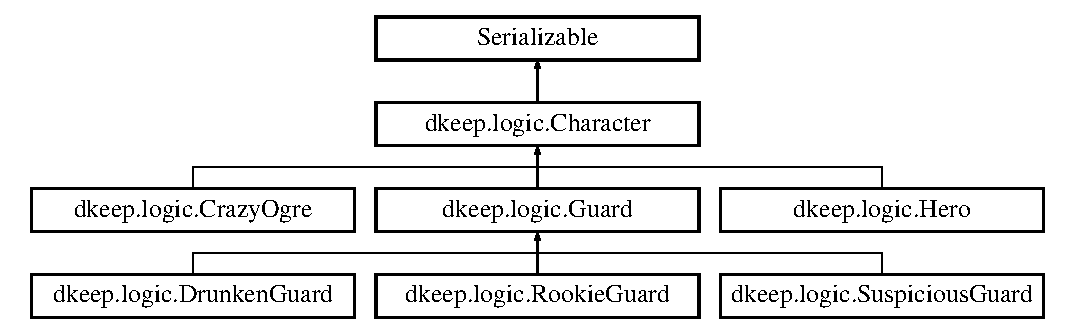
\includegraphics[height=4.000000cm]{classdkeep_1_1logic_1_1_character}
\end{center}
\end{figure}
\subsection*{Public Member Functions}
\begin{DoxyCompactItemize}
\item 
\hyperlink{classdkeep_1_1logic_1_1_character_aae3bf0eb8507fa97aef9e6ece534ea58}{Character} (int\mbox{[}$\,$\mbox{]} coord, char symbol, \hyperlink{classdkeep_1_1logic_1_1_weapon}{Weapon} weapon)
\item 
int \hyperlink{classdkeep_1_1logic_1_1_character_aa8f5ac737dad552c4cffeeaffd2194ec}{getX} ()
\item 
int \hyperlink{classdkeep_1_1logic_1_1_character_a6d872834994ec8c4bea59d1803f3be59}{getY} ()
\item 
void \hyperlink{classdkeep_1_1logic_1_1_character_a5e41fc20fed934fc02bf114f603e540b}{setX} (int x)
\item 
void \hyperlink{classdkeep_1_1logic_1_1_character_aef6651cd827a83c4518e4dcba4ead2b4}{setY} (int y)
\item 
void \hyperlink{classdkeep_1_1logic_1_1_character_a39b7935ecc4b2be1e3070c292d1356bf}{got\+Stunned} ()
\item 
void \hyperlink{classdkeep_1_1logic_1_1_character_afe41039ed701e55162455dd8d480fe2b}{back\+To\+Normal} ()
\item 
abstract char \hyperlink{classdkeep_1_1logic_1_1_character_a8cb0733b49fdd569cc58fe5a3b1a9c29}{get\+Symbol} ()
\item 
\hyperlink{classdkeep_1_1logic_1_1_weapon}{Weapon} \hyperlink{classdkeep_1_1logic_1_1_character_a19d825a86884f725aedd76fdd49ff964}{get\+Weapon} ()
\item 
char \hyperlink{classdkeep_1_1logic_1_1_character_a22be2db9df156acfb3638b3d8826f5ea}{get\+Weapon\+Symbol} ()
\item 
abstract int \mbox{[}$\,$\mbox{]} \hyperlink{classdkeep_1_1logic_1_1_character_a400aadf032a66c591f4ad6ca2660f3f2}{movement} ()
\end{DoxyCompactItemize}
\subsection*{Protected Attributes}
\begin{DoxyCompactItemize}
\item 
\mbox{\Hypertarget{classdkeep_1_1logic_1_1_character_aa1674c0adfcc7425cccd957ce594b8ed}\label{classdkeep_1_1logic_1_1_character_aa1674c0adfcc7425cccd957ce594b8ed}} 
int {\bfseries x}
\item 
\mbox{\Hypertarget{classdkeep_1_1logic_1_1_character_a2b1ff3a7a088a91798ddb264ff37e897}\label{classdkeep_1_1logic_1_1_character_a2b1ff3a7a088a91798ddb264ff37e897}} 
int {\bfseries y}
\item 
\mbox{\Hypertarget{classdkeep_1_1logic_1_1_character_a6ae027052136fb9b1c89851f4ed68fd3}\label{classdkeep_1_1logic_1_1_character_a6ae027052136fb9b1c89851f4ed68fd3}} 
char {\bfseries symbol}
\item 
\mbox{\Hypertarget{classdkeep_1_1logic_1_1_character_ad00f5df3d896d30368c2b25b92452a5b}\label{classdkeep_1_1logic_1_1_character_ad00f5df3d896d30368c2b25b92452a5b}} 
boolean {\bfseries is\+Over\+Key} = false
\item 
\mbox{\Hypertarget{classdkeep_1_1logic_1_1_character_a556deb48a158574080c8e144c80ea1d9}\label{classdkeep_1_1logic_1_1_character_a556deb48a158574080c8e144c80ea1d9}} 
boolean {\bfseries stunned} = false
\item 
\mbox{\Hypertarget{classdkeep_1_1logic_1_1_character_a474a59d32601ec8153b6b751d7fc1b25}\label{classdkeep_1_1logic_1_1_character_a474a59d32601ec8153b6b751d7fc1b25}} 
int {\bfseries turns} = 0
\item 
\mbox{\Hypertarget{classdkeep_1_1logic_1_1_character_a0ce79e6c96b912490371d589c7e8420e}\label{classdkeep_1_1logic_1_1_character_a0ce79e6c96b912490371d589c7e8420e}} 
\hyperlink{classdkeep_1_1logic_1_1_weapon}{Weapon} {\bfseries weapon}
\end{DoxyCompactItemize}


\subsection{Detailed Description}
\hyperlink{classdkeep_1_1logic_1_1_character}{Character} is a class that keeps the information about the moving elements of the game. It keeps information about it\textquotesingle{}s coordinates, symbol, if it\textquotesingle{}s above a key or stunned, it\textquotesingle{}s turns (movement depends on it) and it\textquotesingle{}s weapon. 

\subsection{Constructor \& Destructor Documentation}
\mbox{\Hypertarget{classdkeep_1_1logic_1_1_character_aae3bf0eb8507fa97aef9e6ece534ea58}\label{classdkeep_1_1logic_1_1_character_aae3bf0eb8507fa97aef9e6ece534ea58}} 
\index{dkeep\+::logic\+::\+Character@{dkeep\+::logic\+::\+Character}!Character@{Character}}
\index{Character@{Character}!dkeep\+::logic\+::\+Character@{dkeep\+::logic\+::\+Character}}
\subsubsection{\texorpdfstring{Character()}{Character()}}
{\footnotesize\ttfamily dkeep.\+logic.\+Character.\+Character (\begin{DoxyParamCaption}\item[{int \mbox{[}$\,$\mbox{]}}]{coord,  }\item[{char}]{symbol,  }\item[{\hyperlink{classdkeep_1_1logic_1_1_weapon}{Weapon}}]{weapon }\end{DoxyParamCaption})}

Constructor of \hyperlink{classdkeep_1_1logic_1_1_character}{Character}. Receives it\textquotesingle{}s coordinates, symbol and weapon. 
\begin{DoxyParams}{Parameters}
{\em x} & coordinate \\
\hline
{\em y} & coordinate \\
\hline
{\em symbol} & char that represents the character \\
\hline
{\em weapon} & Object weapon that contains information about the weapon \\
\hline
\end{DoxyParams}


\subsection{Member Function Documentation}
\mbox{\Hypertarget{classdkeep_1_1logic_1_1_character_afe41039ed701e55162455dd8d480fe2b}\label{classdkeep_1_1logic_1_1_character_afe41039ed701e55162455dd8d480fe2b}} 
\index{dkeep\+::logic\+::\+Character@{dkeep\+::logic\+::\+Character}!back\+To\+Normal@{back\+To\+Normal}}
\index{back\+To\+Normal@{back\+To\+Normal}!dkeep\+::logic\+::\+Character@{dkeep\+::logic\+::\+Character}}
\subsubsection{\texorpdfstring{back\+To\+Normal()}{backToNormal()}}
{\footnotesize\ttfamily void dkeep.\+logic.\+Character.\+back\+To\+Normal (\begin{DoxyParamCaption}{ }\end{DoxyParamCaption})}

Puts the flag stunned back to false. Happens when the number of turns has reached 0. \mbox{\Hypertarget{classdkeep_1_1logic_1_1_character_a8cb0733b49fdd569cc58fe5a3b1a9c29}\label{classdkeep_1_1logic_1_1_character_a8cb0733b49fdd569cc58fe5a3b1a9c29}} 
\index{dkeep\+::logic\+::\+Character@{dkeep\+::logic\+::\+Character}!get\+Symbol@{get\+Symbol}}
\index{get\+Symbol@{get\+Symbol}!dkeep\+::logic\+::\+Character@{dkeep\+::logic\+::\+Character}}
\subsubsection{\texorpdfstring{get\+Symbol()}{getSymbol()}}
{\footnotesize\ttfamily abstract char dkeep.\+logic.\+Character.\+get\+Symbol (\begin{DoxyParamCaption}{ }\end{DoxyParamCaption})\hspace{0.3cm}{\ttfamily [abstract]}}

Returns the symbol of the \hyperlink{classdkeep_1_1logic_1_1_character}{Character}, depending on it\textquotesingle{}s state and qualities. \begin{DoxyReturn}{Returns}
char representing it\textquotesingle{}s display on the game 
\end{DoxyReturn}
\mbox{\Hypertarget{classdkeep_1_1logic_1_1_character_a19d825a86884f725aedd76fdd49ff964}\label{classdkeep_1_1logic_1_1_character_a19d825a86884f725aedd76fdd49ff964}} 
\index{dkeep\+::logic\+::\+Character@{dkeep\+::logic\+::\+Character}!get\+Weapon@{get\+Weapon}}
\index{get\+Weapon@{get\+Weapon}!dkeep\+::logic\+::\+Character@{dkeep\+::logic\+::\+Character}}
\subsubsection{\texorpdfstring{get\+Weapon()}{getWeapon()}}
{\footnotesize\ttfamily \hyperlink{classdkeep_1_1logic_1_1_weapon}{Weapon} dkeep.\+logic.\+Character.\+get\+Weapon (\begin{DoxyParamCaption}{ }\end{DoxyParamCaption})}

Retrieve the weapon of the character. If null, it will return null \begin{DoxyReturn}{Returns}
weapon of the character, Object \hyperlink{classdkeep_1_1logic_1_1_weapon}{Weapon} 
\end{DoxyReturn}
\mbox{\Hypertarget{classdkeep_1_1logic_1_1_character_a22be2db9df156acfb3638b3d8826f5ea}\label{classdkeep_1_1logic_1_1_character_a22be2db9df156acfb3638b3d8826f5ea}} 
\index{dkeep\+::logic\+::\+Character@{dkeep\+::logic\+::\+Character}!get\+Weapon\+Symbol@{get\+Weapon\+Symbol}}
\index{get\+Weapon\+Symbol@{get\+Weapon\+Symbol}!dkeep\+::logic\+::\+Character@{dkeep\+::logic\+::\+Character}}
\subsubsection{\texorpdfstring{get\+Weapon\+Symbol()}{getWeaponSymbol()}}
{\footnotesize\ttfamily char dkeep.\+logic.\+Character.\+get\+Weapon\+Symbol (\begin{DoxyParamCaption}{ }\end{DoxyParamCaption})}

Retrieve the weapon char depending on it\textquotesingle{}s state. If weapon is null, it will return a char with empty space. \begin{DoxyReturn}{Returns}
char representing the weapon symbol 
\end{DoxyReturn}
\mbox{\Hypertarget{classdkeep_1_1logic_1_1_character_aa8f5ac737dad552c4cffeeaffd2194ec}\label{classdkeep_1_1logic_1_1_character_aa8f5ac737dad552c4cffeeaffd2194ec}} 
\index{dkeep\+::logic\+::\+Character@{dkeep\+::logic\+::\+Character}!getX@{getX}}
\index{getX@{getX}!dkeep\+::logic\+::\+Character@{dkeep\+::logic\+::\+Character}}
\subsubsection{\texorpdfstring{get\+X()}{getX()}}
{\footnotesize\ttfamily int dkeep.\+logic.\+Character.\+getX (\begin{DoxyParamCaption}{ }\end{DoxyParamCaption})}

Retrieve the valor of the coordinate x. \begin{DoxyReturn}{Returns}
the coordinate x, type int 
\end{DoxyReturn}
\mbox{\Hypertarget{classdkeep_1_1logic_1_1_character_a6d872834994ec8c4bea59d1803f3be59}\label{classdkeep_1_1logic_1_1_character_a6d872834994ec8c4bea59d1803f3be59}} 
\index{dkeep\+::logic\+::\+Character@{dkeep\+::logic\+::\+Character}!getY@{getY}}
\index{getY@{getY}!dkeep\+::logic\+::\+Character@{dkeep\+::logic\+::\+Character}}
\subsubsection{\texorpdfstring{get\+Y()}{getY()}}
{\footnotesize\ttfamily int dkeep.\+logic.\+Character.\+getY (\begin{DoxyParamCaption}{ }\end{DoxyParamCaption})}

Retrieve the valor of the coordinate y. \begin{DoxyReturn}{Returns}
the coordinate y, type int 
\end{DoxyReturn}
\mbox{\Hypertarget{classdkeep_1_1logic_1_1_character_a39b7935ecc4b2be1e3070c292d1356bf}\label{classdkeep_1_1logic_1_1_character_a39b7935ecc4b2be1e3070c292d1356bf}} 
\index{dkeep\+::logic\+::\+Character@{dkeep\+::logic\+::\+Character}!got\+Stunned@{got\+Stunned}}
\index{got\+Stunned@{got\+Stunned}!dkeep\+::logic\+::\+Character@{dkeep\+::logic\+::\+Character}}
\subsubsection{\texorpdfstring{got\+Stunned()}{gotStunned()}}
{\footnotesize\ttfamily void dkeep.\+logic.\+Character.\+got\+Stunned (\begin{DoxyParamCaption}{ }\end{DoxyParamCaption})}

Puts the flag stunned true and updates the turns to 2. Only happens for enemies if they got \char`\"{}hit\char`\"{} with the hero weapon. \mbox{\Hypertarget{classdkeep_1_1logic_1_1_character_a400aadf032a66c591f4ad6ca2660f3f2}\label{classdkeep_1_1logic_1_1_character_a400aadf032a66c591f4ad6ca2660f3f2}} 
\index{dkeep\+::logic\+::\+Character@{dkeep\+::logic\+::\+Character}!movement@{movement}}
\index{movement@{movement}!dkeep\+::logic\+::\+Character@{dkeep\+::logic\+::\+Character}}
\subsubsection{\texorpdfstring{movement()}{movement()}}
{\footnotesize\ttfamily abstract int \mbox{[}$\,$\mbox{]} dkeep.\+logic.\+Character.\+movement (\begin{DoxyParamCaption}{ }\end{DoxyParamCaption})\hspace{0.3cm}{\ttfamily [abstract]}}

Retrieve a array on 2 ints with the possible new coordinates x and y of the character. \begin{DoxyReturn}{Returns}
array of 2 ints with the coordinates x and y 
\end{DoxyReturn}
\mbox{\Hypertarget{classdkeep_1_1logic_1_1_character_a5e41fc20fed934fc02bf114f603e540b}\label{classdkeep_1_1logic_1_1_character_a5e41fc20fed934fc02bf114f603e540b}} 
\index{dkeep\+::logic\+::\+Character@{dkeep\+::logic\+::\+Character}!setX@{setX}}
\index{setX@{setX}!dkeep\+::logic\+::\+Character@{dkeep\+::logic\+::\+Character}}
\subsubsection{\texorpdfstring{set\+X()}{setX()}}
{\footnotesize\ttfamily void dkeep.\+logic.\+Character.\+setX (\begin{DoxyParamCaption}\item[{int}]{x }\end{DoxyParamCaption})}

Set the coordinate x to the value given. 
\begin{DoxyParams}{Parameters}
{\em x} & new coordinate to be updated \\
\hline
\end{DoxyParams}
\mbox{\Hypertarget{classdkeep_1_1logic_1_1_character_aef6651cd827a83c4518e4dcba4ead2b4}\label{classdkeep_1_1logic_1_1_character_aef6651cd827a83c4518e4dcba4ead2b4}} 
\index{dkeep\+::logic\+::\+Character@{dkeep\+::logic\+::\+Character}!setY@{setY}}
\index{setY@{setY}!dkeep\+::logic\+::\+Character@{dkeep\+::logic\+::\+Character}}
\subsubsection{\texorpdfstring{set\+Y()}{setY()}}
{\footnotesize\ttfamily void dkeep.\+logic.\+Character.\+setY (\begin{DoxyParamCaption}\item[{int}]{y }\end{DoxyParamCaption})}

Set the coordinate y to the value given. 
\begin{DoxyParams}{Parameters}
{\em y} & new coordinate to be updated \\
\hline
\end{DoxyParams}


The documentation for this class was generated from the following file\+:\begin{DoxyCompactItemize}
\item 
C\+:/\+Users/\+M\+C-\/\+Guida/git/\+L\+P\+O\+O1617\+\_\+\+T1\+G5/\+Lab05/src/dkeep/logic/Character.\+java\end{DoxyCompactItemize}

\hypertarget{classdkeep_1_1logic_1_1_club}{}\section{dkeep.\+logic.\+Club Class Reference}
\label{classdkeep_1_1logic_1_1_club}\index{dkeep.\+logic.\+Club@{dkeep.\+logic.\+Club}}
Inheritance diagram for dkeep.\+logic.\+Club\+:\begin{figure}[H]
\begin{center}
\leavevmode
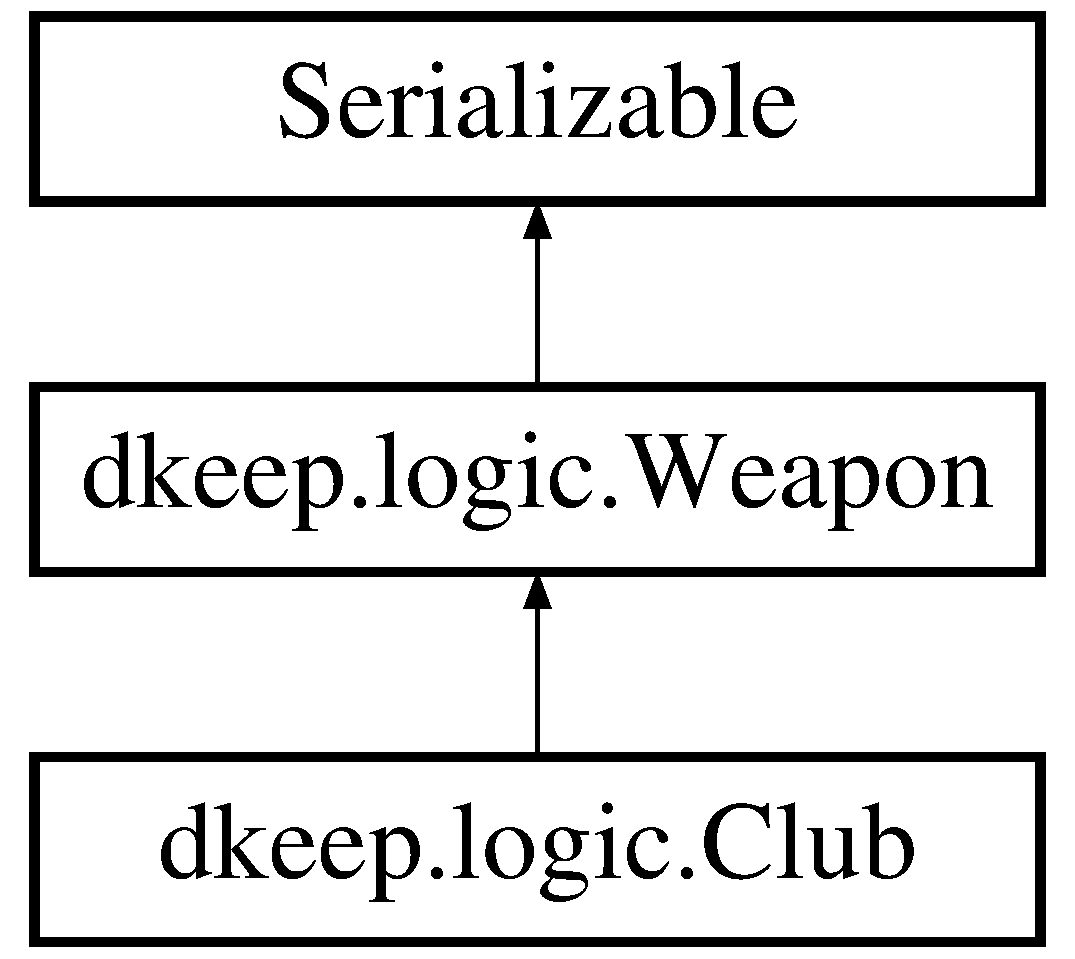
\includegraphics[height=3.000000cm]{classdkeep_1_1logic_1_1_club}
\end{center}
\end{figure}
\subsection*{Public Member Functions}
\begin{DoxyCompactItemize}
\item 
\hyperlink{classdkeep_1_1logic_1_1_club_a214c1629b02c86c58ee5cc6c73e26e2c}{Club} (char symbol, char secsymbol, int\mbox{[}$\,$\mbox{]} coord)
\item 
int \mbox{[}$\,$\mbox{]} \hyperlink{classdkeep_1_1logic_1_1_club_a11ee654cc6aea04eb87aad2f4e8b3edb}{swing} (int x, int y)
\end{DoxyCompactItemize}
\subsection*{Additional Inherited Members}


\subsection{Detailed Description}
\hyperlink{classdkeep_1_1logic_1_1_club}{Club} is a class that extends class \hyperlink{classdkeep_1_1logic_1_1_weapon}{Weapon}, meaning that is a type of weapon that can be \char`\"{}used\char`\"{} by a \hyperlink{classdkeep_1_1logic_1_1_character}{Character}. This particular weapon as a specific symbol. \begin{DoxySeeAlso}{See also}
\hyperlink{classdkeep_1_1logic_1_1_weapon}{Weapon} 
\end{DoxySeeAlso}


\subsection{Constructor \& Destructor Documentation}
\mbox{\Hypertarget{classdkeep_1_1logic_1_1_club_a214c1629b02c86c58ee5cc6c73e26e2c}\label{classdkeep_1_1logic_1_1_club_a214c1629b02c86c58ee5cc6c73e26e2c}} 
\index{dkeep\+::logic\+::\+Club@{dkeep\+::logic\+::\+Club}!Club@{Club}}
\index{Club@{Club}!dkeep\+::logic\+::\+Club@{dkeep\+::logic\+::\+Club}}
\subsubsection{\texorpdfstring{Club()}{Club()}}
{\footnotesize\ttfamily dkeep.\+logic.\+Club.\+Club (\begin{DoxyParamCaption}\item[{char}]{symbol,  }\item[{char}]{secsymbol,  }\item[{int \mbox{[}$\,$\mbox{]}}]{coord }\end{DoxyParamCaption})}

Constructor of \hyperlink{classdkeep_1_1logic_1_1_club}{Club}. Sets all flags to false and initializes all data with the given values. 
\begin{DoxyParams}{Parameters}
{\em symbol} & char that represents the \hyperlink{classdkeep_1_1logic_1_1_club}{Club} in it\textquotesingle{}s default status \\
\hline
{\em secsymbol} & char that represents the \hyperlink{classdkeep_1_1logic_1_1_club}{Club} in certain situations \\
\hline
{\em x} & coordinate \\
\hline
{\em y} & coordinate \\
\hline
\end{DoxyParams}


\subsection{Member Function Documentation}
\mbox{\Hypertarget{classdkeep_1_1logic_1_1_club_a11ee654cc6aea04eb87aad2f4e8b3edb}\label{classdkeep_1_1logic_1_1_club_a11ee654cc6aea04eb87aad2f4e8b3edb}} 
\index{dkeep\+::logic\+::\+Club@{dkeep\+::logic\+::\+Club}!swing@{swing}}
\index{swing@{swing}!dkeep\+::logic\+::\+Club@{dkeep\+::logic\+::\+Club}}
\subsubsection{\texorpdfstring{swing()}{swing()}}
{\footnotesize\ttfamily int \mbox{[}$\,$\mbox{]} dkeep.\+logic.\+Club.\+swing (\begin{DoxyParamCaption}\item[{int}]{x,  }\item[{int}]{y }\end{DoxyParamCaption})}



The documentation for this class was generated from the following file\+:\begin{DoxyCompactItemize}
\item 
C\+:/\+Users/\+M\+C-\/\+Guida/git/\+L\+P\+O\+O1617\+\_\+\+T1\+G5/\+Lab05/src/dkeep/logic/Club.\+java\end{DoxyCompactItemize}

\hypertarget{classdkeep_1_1logic_1_1_crazy_ogre}{}\section{dkeep.\+logic.\+Crazy\+Ogre Class Reference}
\label{classdkeep_1_1logic_1_1_crazy_ogre}\index{dkeep.\+logic.\+Crazy\+Ogre@{dkeep.\+logic.\+Crazy\+Ogre}}
Inheritance diagram for dkeep.\+logic.\+Crazy\+Ogre\+:\begin{figure}[H]
\begin{center}
\leavevmode
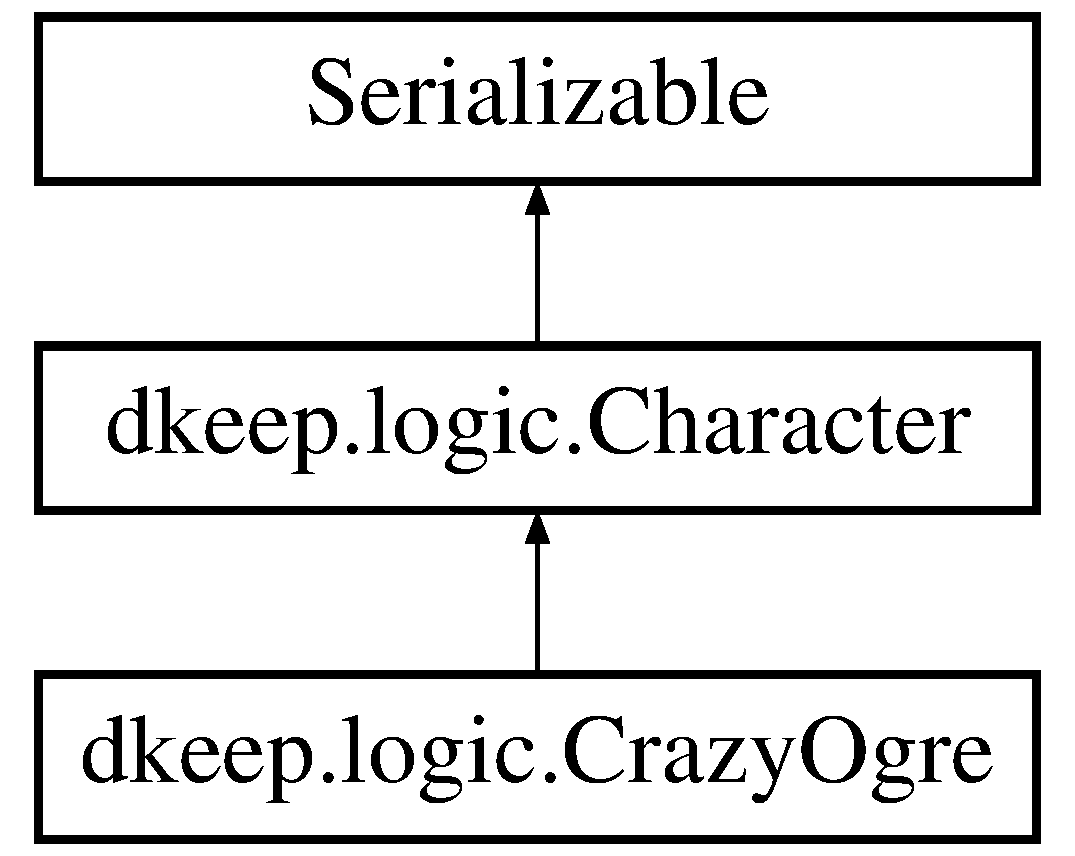
\includegraphics[height=3.000000cm]{classdkeep_1_1logic_1_1_crazy_ogre}
\end{center}
\end{figure}
\subsection*{Public Member Functions}
\begin{DoxyCompactItemize}
\item 
\hyperlink{classdkeep_1_1logic_1_1_crazy_ogre_a80eeff663b6b50957cb22dfd0f738a8e}{Crazy\+Ogre} (char symbol, int\mbox{[}$\,$\mbox{]} coord, \hyperlink{classdkeep_1_1logic_1_1_weapon}{Weapon} weapon)
\item 
int \mbox{[}$\,$\mbox{]} \hyperlink{classdkeep_1_1logic_1_1_crazy_ogre_a4b12a877e7adb6af8b40d987f0b37e8c}{movement} ()
\item 
char \hyperlink{classdkeep_1_1logic_1_1_crazy_ogre_af1bf05bce7387b6ac6800d7b4290565c}{get\+Symbol} ()
\end{DoxyCompactItemize}
\subsection*{Additional Inherited Members}


\subsection{Detailed Description}
\hyperlink{classdkeep_1_1logic_1_1_crazy_ogre}{Crazy\+Ogre} is a class that keeps information about the enemy \hyperlink{classdkeep_1_1logic_1_1_crazy_ogre}{Crazy\+Ogre} of the game. This enemy has a symbol, coordinates x and y, two booleans representing if he is in the same position of the key and if it is stunned (was it by the hero weapon).It also keeps information about the turns it still has to wait while stunned and it\textquotesingle{}s weapon.

\begin{DoxySeeAlso}{See also}
\hyperlink{classdkeep_1_1logic_1_1_character}{Character} 
\end{DoxySeeAlso}


\subsection{Constructor \& Destructor Documentation}
\mbox{\Hypertarget{classdkeep_1_1logic_1_1_crazy_ogre_a80eeff663b6b50957cb22dfd0f738a8e}\label{classdkeep_1_1logic_1_1_crazy_ogre_a80eeff663b6b50957cb22dfd0f738a8e}} 
\index{dkeep\+::logic\+::\+Crazy\+Ogre@{dkeep\+::logic\+::\+Crazy\+Ogre}!Crazy\+Ogre@{Crazy\+Ogre}}
\index{Crazy\+Ogre@{Crazy\+Ogre}!dkeep\+::logic\+::\+Crazy\+Ogre@{dkeep\+::logic\+::\+Crazy\+Ogre}}
\subsubsection{\texorpdfstring{Crazy\+Ogre()}{CrazyOgre()}}
{\footnotesize\ttfamily dkeep.\+logic.\+Crazy\+Ogre.\+Crazy\+Ogre (\begin{DoxyParamCaption}\item[{char}]{symbol,  }\item[{int \mbox{[}$\,$\mbox{]}}]{coord,  }\item[{\hyperlink{classdkeep_1_1logic_1_1_weapon}{Weapon}}]{weapon }\end{DoxyParamCaption})}

Constructor of \hyperlink{classdkeep_1_1logic_1_1_crazy_ogre}{Crazy\+Ogre}. Receives it\textquotesingle{}s coordinates, it\textquotesingle{}s symbol and the weapon, that could possibly be null or a \hyperlink{classdkeep_1_1logic_1_1_club}{Club}. 
\begin{DoxyParams}{Parameters}
{\em symbol} & char that will represent the ogre \\
\hline
{\em x} & coordinate \\
\hline
{\em y} & coordinate \\
\hline
{\em weapon} & object \hyperlink{classdkeep_1_1logic_1_1_weapon}{Weapon} that contains information about a \hyperlink{classdkeep_1_1logic_1_1_club}{Club} \\
\hline
\end{DoxyParams}


\subsection{Member Function Documentation}
\mbox{\Hypertarget{classdkeep_1_1logic_1_1_crazy_ogre_af1bf05bce7387b6ac6800d7b4290565c}\label{classdkeep_1_1logic_1_1_crazy_ogre_af1bf05bce7387b6ac6800d7b4290565c}} 
\index{dkeep\+::logic\+::\+Crazy\+Ogre@{dkeep\+::logic\+::\+Crazy\+Ogre}!get\+Symbol@{get\+Symbol}}
\index{get\+Symbol@{get\+Symbol}!dkeep\+::logic\+::\+Crazy\+Ogre@{dkeep\+::logic\+::\+Crazy\+Ogre}}
\subsubsection{\texorpdfstring{get\+Symbol()}{getSymbol()}}
{\footnotesize\ttfamily char dkeep.\+logic.\+Crazy\+Ogre.\+get\+Symbol (\begin{DoxyParamCaption}{ }\end{DoxyParamCaption})}

If the Ogre is in the same position has the key or if it is stunned, it symbol is different that the default one. \mbox{\Hypertarget{classdkeep_1_1logic_1_1_crazy_ogre_a4b12a877e7adb6af8b40d987f0b37e8c}\label{classdkeep_1_1logic_1_1_crazy_ogre_a4b12a877e7adb6af8b40d987f0b37e8c}} 
\index{dkeep\+::logic\+::\+Crazy\+Ogre@{dkeep\+::logic\+::\+Crazy\+Ogre}!movement@{movement}}
\index{movement@{movement}!dkeep\+::logic\+::\+Crazy\+Ogre@{dkeep\+::logic\+::\+Crazy\+Ogre}}
\subsubsection{\texorpdfstring{movement()}{movement()}}
{\footnotesize\ttfamily int \mbox{[}$\,$\mbox{]} dkeep.\+logic.\+Crazy\+Ogre.\+movement (\begin{DoxyParamCaption}{ }\end{DoxyParamCaption})}

It randomly chooses between one of 4 directions and calculates the respective coordinates based on the actual ones, then returns the calculated coordinates. 

The documentation for this class was generated from the following file\+:\begin{DoxyCompactItemize}
\item 
C\+:/\+Users/\+M\+C-\/\+Guida/git/\+L\+P\+O\+O1617\+\_\+\+T1\+G5/\+Lab05/src/dkeep/logic/Crazy\+Ogre.\+java\end{DoxyCompactItemize}

\hypertarget{classdkeep_1_1logic_1_1_drunken_guard}{}\section{dkeep.\+logic.\+Drunken\+Guard Class Reference}
\label{classdkeep_1_1logic_1_1_drunken_guard}\index{dkeep.\+logic.\+Drunken\+Guard@{dkeep.\+logic.\+Drunken\+Guard}}
Inheritance diagram for dkeep.\+logic.\+Drunken\+Guard\+:\begin{figure}[H]
\begin{center}
\leavevmode
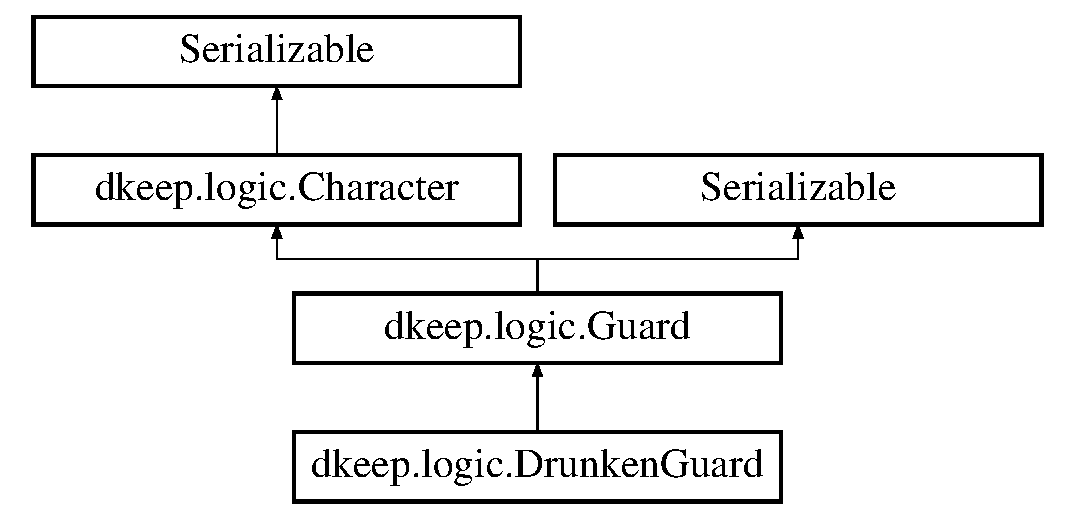
\includegraphics[height=4.000000cm]{classdkeep_1_1logic_1_1_drunken_guard}
\end{center}
\end{figure}
\subsection*{Public Member Functions}
\begin{DoxyCompactItemize}
\item 
\hyperlink{classdkeep_1_1logic_1_1_drunken_guard_a8779127a311ed0f350abb672304854db}{Drunken\+Guard} (char symbol, int\mbox{[}$\,$\mbox{]} coord, char\mbox{[}$\,$\mbox{]} path)
\item 
int \mbox{[}$\,$\mbox{]} \hyperlink{classdkeep_1_1logic_1_1_drunken_guard_ade9c30f28e40df9049472a5807c2b79e}{movement} ()
\item 
char \hyperlink{classdkeep_1_1logic_1_1_drunken_guard_a03c948e95e3c62b9708b4c5a6b8770f8}{get\+Symbol} ()
\end{DoxyCompactItemize}
\subsection*{Additional Inherited Members}


\subsection{Detailed Description}
\hyperlink{classdkeep_1_1logic_1_1_drunken_guard}{Drunken\+Guard} is a class that extend the class \hyperlink{classdkeep_1_1logic_1_1_guard}{Guard}. It contains specific information about this type of guard, such as the boolean that says if the guard is asleep and the corresponding char that expresses that status. This guard randomly chooses to follows the normal path, the reverse path or to be asleep. This last one consist of staying in the same position, changing it\textquotesingle{}s symbol and being unaware of the hero movements, even in the adjacent tiles. \begin{DoxySeeAlso}{See also}
\hyperlink{classdkeep_1_1logic_1_1_guard}{Guard} 
\end{DoxySeeAlso}


\subsection{Constructor \& Destructor Documentation}
\mbox{\Hypertarget{classdkeep_1_1logic_1_1_drunken_guard_a8779127a311ed0f350abb672304854db}\label{classdkeep_1_1logic_1_1_drunken_guard_a8779127a311ed0f350abb672304854db}} 
\index{dkeep\+::logic\+::\+Drunken\+Guard@{dkeep\+::logic\+::\+Drunken\+Guard}!Drunken\+Guard@{Drunken\+Guard}}
\index{Drunken\+Guard@{Drunken\+Guard}!dkeep\+::logic\+::\+Drunken\+Guard@{dkeep\+::logic\+::\+Drunken\+Guard}}
\subsubsection{\texorpdfstring{Drunken\+Guard()}{DrunkenGuard()}}
{\footnotesize\ttfamily dkeep.\+logic.\+Drunken\+Guard.\+Drunken\+Guard (\begin{DoxyParamCaption}\item[{char}]{symbol,  }\item[{int \mbox{[}$\,$\mbox{]}}]{coord,  }\item[{char \mbox{[}$\,$\mbox{]}}]{path }\end{DoxyParamCaption})}

Constructor of \hyperlink{classdkeep_1_1logic_1_1_drunken_guard}{Drunken\+Guard}. Sets all flags to false, puts the i variable to -\/1 and initializes other variables with the given values. 
\begin{DoxyParams}{Parameters}
{\em symbol} & char that represents the \hyperlink{classdkeep_1_1logic_1_1_drunken_guard}{Drunken\+Guard} \\
\hline
{\em x} & coordinate \\
\hline
{\em y} & coordinate \\
\hline
{\em path} & array of movements of the guard \\
\hline
\end{DoxyParams}


\subsection{Member Function Documentation}
\mbox{\Hypertarget{classdkeep_1_1logic_1_1_drunken_guard_a03c948e95e3c62b9708b4c5a6b8770f8}\label{classdkeep_1_1logic_1_1_drunken_guard_a03c948e95e3c62b9708b4c5a6b8770f8}} 
\index{dkeep\+::logic\+::\+Drunken\+Guard@{dkeep\+::logic\+::\+Drunken\+Guard}!get\+Symbol@{get\+Symbol}}
\index{get\+Symbol@{get\+Symbol}!dkeep\+::logic\+::\+Drunken\+Guard@{dkeep\+::logic\+::\+Drunken\+Guard}}
\subsubsection{\texorpdfstring{get\+Symbol()}{getSymbol()}}
{\footnotesize\ttfamily char dkeep.\+logic.\+Drunken\+Guard.\+get\+Symbol (\begin{DoxyParamCaption}{ }\end{DoxyParamCaption})}

If the guard is asleep, the symbol is different. \mbox{\Hypertarget{classdkeep_1_1logic_1_1_drunken_guard_ade9c30f28e40df9049472a5807c2b79e}\label{classdkeep_1_1logic_1_1_drunken_guard_ade9c30f28e40df9049472a5807c2b79e}} 
\index{dkeep\+::logic\+::\+Drunken\+Guard@{dkeep\+::logic\+::\+Drunken\+Guard}!movement@{movement}}
\index{movement@{movement}!dkeep\+::logic\+::\+Drunken\+Guard@{dkeep\+::logic\+::\+Drunken\+Guard}}
\subsubsection{\texorpdfstring{movement()}{movement()}}
{\footnotesize\ttfamily int \mbox{[}$\,$\mbox{]} dkeep.\+logic.\+Drunken\+Guard.\+movement (\begin{DoxyParamCaption}{ }\end{DoxyParamCaption})}

in this particular class, this function randomly chooses between 3 behaviours, the normal one (follows the path and calls the \hyperlink{classdkeep_1_1logic_1_1_guard_a2389016085c6d65d4366930fac72dab4}{normal\+Movement()} function), the reverse one (follows the path in reverse order, calls the \hyperlink{classdkeep_1_1logic_1_1_guard_a8c588aa887fcfe6d3e4a9e13d236c644}{reverse\+Movement()} function) and the asleep one, that puts the enemy in a temporary status of 2 turns, making it oblivious to the hero movements. 

The documentation for this class was generated from the following file\+:\begin{DoxyCompactItemize}
\item 
C\+:/\+Users/\+M\+C-\/\+Guida/git/\+L\+P\+O\+O1617\+\_\+\+T1\+G5/\+Lab05/src/dkeep/logic/Drunken\+Guard.\+java\end{DoxyCompactItemize}

\hypertarget{classdkeep_1_1logic_1_1_dungeon_logic}{}\section{dkeep.\+logic.\+Dungeon\+Logic Class Reference}
\label{classdkeep_1_1logic_1_1_dungeon_logic}\index{dkeep.\+logic.\+Dungeon\+Logic@{dkeep.\+logic.\+Dungeon\+Logic}}
Inheritance diagram for dkeep.\+logic.\+Dungeon\+Logic\+:\begin{figure}[H]
\begin{center}
\leavevmode
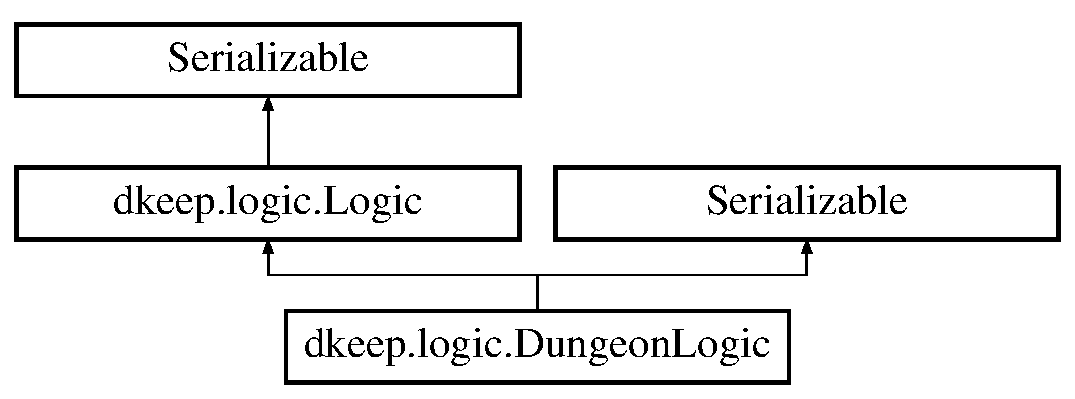
\includegraphics[height=3.000000cm]{classdkeep_1_1logic_1_1_dungeon_logic}
\end{center}
\end{figure}
\subsection*{Public Member Functions}
\begin{DoxyCompactItemize}
\item 
\hyperlink{classdkeep_1_1logic_1_1_dungeon_logic_a705c692038bc3af07788e0091f9176b7}{Dungeon\+Logic} (\hyperlink{classdkeep_1_1logic_1_1_map}{Map} map, int\mbox{[}$\,$\mbox{]} heropos, int option)
\item 
boolean \hyperlink{classdkeep_1_1logic_1_1_dungeon_logic_a5560298a8a9e7831ce61a8cc1a7bc7c4}{move\+Hero} (char dir, \hyperlink{classdkeep_1_1logic_1_1_map}{Map} map)
\item 
void \hyperlink{classdkeep_1_1logic_1_1_dungeon_logic_a94e25841318f6c9f82bd7f1654b7368a}{gameplay} (char dir, \hyperlink{classdkeep_1_1logic_1_1_map}{Map} map)
\item 
\hyperlink{classdkeep_1_1logic_1_1_logic}{Logic} \hyperlink{classdkeep_1_1logic_1_1_dungeon_logic_ae94692c5c7044d32f78d2e021b0a9513}{next\+Logic} (\hyperlink{classdkeep_1_1logic_1_1_map}{Map} map, int option)
\end{DoxyCompactItemize}
\subsection*{Additional Inherited Members}


\subsection{Detailed Description}
\hyperlink{classdkeep_1_1logic_1_1_dungeon_logic}{Dungeon\+Logic} is a class that extends \hyperlink{classdkeep_1_1logic_1_1_logic}{Logic} and it\textquotesingle{}s function is to deal with the logic of the Dungeon level. It contains all the specific functions that deal with the hero and the type of enemies of its level. The big difference in this class, compared to the other, is the existence of three guards, each with a different behaviour. This level only has a lever. \begin{DoxySeeAlso}{See also}
\hyperlink{classdkeep_1_1logic_1_1_logic}{Logic} 
\end{DoxySeeAlso}


\subsection{Constructor \& Destructor Documentation}
\mbox{\Hypertarget{classdkeep_1_1logic_1_1_dungeon_logic_a705c692038bc3af07788e0091f9176b7}\label{classdkeep_1_1logic_1_1_dungeon_logic_a705c692038bc3af07788e0091f9176b7}} 
\index{dkeep\+::logic\+::\+Dungeon\+Logic@{dkeep\+::logic\+::\+Dungeon\+Logic}!Dungeon\+Logic@{Dungeon\+Logic}}
\index{Dungeon\+Logic@{Dungeon\+Logic}!dkeep\+::logic\+::\+Dungeon\+Logic@{dkeep\+::logic\+::\+Dungeon\+Logic}}
\subsubsection{\texorpdfstring{Dungeon\+Logic()}{DungeonLogic()}}
{\footnotesize\ttfamily dkeep.\+logic.\+Dungeon\+Logic.\+Dungeon\+Logic (\begin{DoxyParamCaption}\item[{\hyperlink{classdkeep_1_1logic_1_1_map}{Map}}]{map,  }\item[{int \mbox{[}$\,$\mbox{]}}]{heropos,  }\item[{int}]{option }\end{DoxyParamCaption})}

Constructor of \hyperlink{classdkeep_1_1logic_1_1_dungeon_logic}{Dungeon\+Logic}. It calls the \hyperlink{classdkeep_1_1logic_1_1_logic}{Logic} constructor, then adds one enemy, which behaviour is chosen according to the option selected by the user. The path is always the same. 
\begin{DoxyParams}{Parameters}
{\em map} & \hyperlink{classdkeep_1_1logic_1_1_map}{Map} of the current level \\
\hline
{\em heropos} & starting position of the hero \\
\hline
{\em option} & refers to the behaviour of the guard \\
\hline
\end{DoxyParams}


\subsection{Member Function Documentation}
\mbox{\Hypertarget{classdkeep_1_1logic_1_1_dungeon_logic_a94e25841318f6c9f82bd7f1654b7368a}\label{classdkeep_1_1logic_1_1_dungeon_logic_a94e25841318f6c9f82bd7f1654b7368a}} 
\index{dkeep\+::logic\+::\+Dungeon\+Logic@{dkeep\+::logic\+::\+Dungeon\+Logic}!gameplay@{gameplay}}
\index{gameplay@{gameplay}!dkeep\+::logic\+::\+Dungeon\+Logic@{dkeep\+::logic\+::\+Dungeon\+Logic}}
\subsubsection{\texorpdfstring{gameplay()}{gameplay()}}
{\footnotesize\ttfamily void dkeep.\+logic.\+Dungeon\+Logic.\+gameplay (\begin{DoxyParamCaption}\item[{char}]{dir,  }\item[{\hyperlink{classdkeep_1_1logic_1_1_map}{Map}}]{map }\end{DoxyParamCaption})}

In this level, only the enemy and hero movements are made because there are no weapons. \mbox{\Hypertarget{classdkeep_1_1logic_1_1_dungeon_logic_a5560298a8a9e7831ce61a8cc1a7bc7c4}\label{classdkeep_1_1logic_1_1_dungeon_logic_a5560298a8a9e7831ce61a8cc1a7bc7c4}} 
\index{dkeep\+::logic\+::\+Dungeon\+Logic@{dkeep\+::logic\+::\+Dungeon\+Logic}!move\+Hero@{move\+Hero}}
\index{move\+Hero@{move\+Hero}!dkeep\+::logic\+::\+Dungeon\+Logic@{dkeep\+::logic\+::\+Dungeon\+Logic}}
\subsubsection{\texorpdfstring{move\+Hero()}{moveHero()}}
{\footnotesize\ttfamily boolean dkeep.\+logic.\+Dungeon\+Logic.\+move\+Hero (\begin{DoxyParamCaption}\item[{char}]{dir,  }\item[{\hyperlink{classdkeep_1_1logic_1_1_map}{Map}}]{map }\end{DoxyParamCaption})}

\mbox{\Hypertarget{classdkeep_1_1logic_1_1_dungeon_logic_ae94692c5c7044d32f78d2e021b0a9513}\label{classdkeep_1_1logic_1_1_dungeon_logic_ae94692c5c7044d32f78d2e021b0a9513}} 
\index{dkeep\+::logic\+::\+Dungeon\+Logic@{dkeep\+::logic\+::\+Dungeon\+Logic}!next\+Logic@{next\+Logic}}
\index{next\+Logic@{next\+Logic}!dkeep\+::logic\+::\+Dungeon\+Logic@{dkeep\+::logic\+::\+Dungeon\+Logic}}
\subsubsection{\texorpdfstring{next\+Logic()}{nextLogic()}}
{\footnotesize\ttfamily \hyperlink{classdkeep_1_1logic_1_1_logic}{Logic} dkeep.\+logic.\+Dungeon\+Logic.\+next\+Logic (\begin{DoxyParamCaption}\item[{\hyperlink{classdkeep_1_1logic_1_1_map}{Map}}]{map,  }\item[{int}]{option }\end{DoxyParamCaption})}



The documentation for this class was generated from the following file\+:\begin{DoxyCompactItemize}
\item 
C\+:/\+Users/\+M\+C-\/\+Guida/git/\+L\+P\+O\+O1617\+\_\+\+T1\+G5/\+Lab05/src/dkeep/logic/Dungeon\+Logic.\+java\end{DoxyCompactItemize}

\hypertarget{classdkeep_1_1logic_1_1_dungeon_map}{}\section{dkeep.\+logic.\+Dungeon\+Map Class Reference}
\label{classdkeep_1_1logic_1_1_dungeon_map}\index{dkeep.\+logic.\+Dungeon\+Map@{dkeep.\+logic.\+Dungeon\+Map}}
Inheritance diagram for dkeep.\+logic.\+Dungeon\+Map\+:\begin{figure}[H]
\begin{center}
\leavevmode
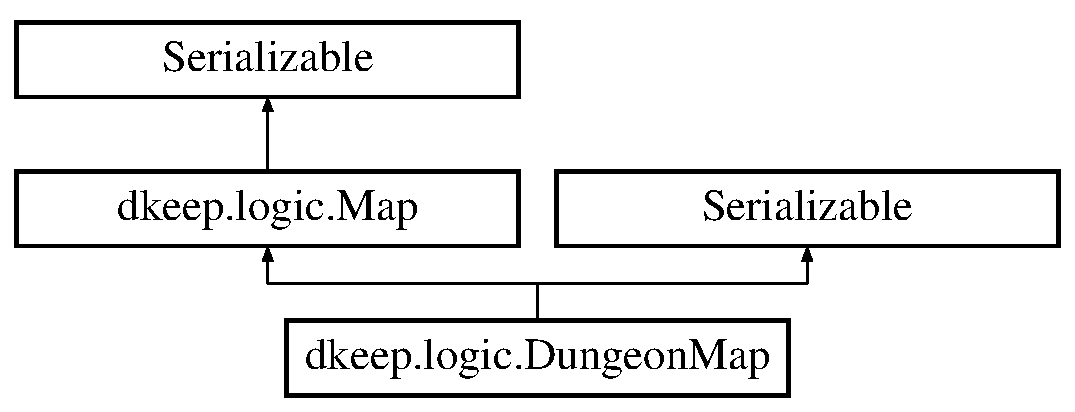
\includegraphics[height=3.000000cm]{classdkeep_1_1logic_1_1_dungeon_map}
\end{center}
\end{figure}
\subsection*{Public Member Functions}
\begin{DoxyCompactItemize}
\item 
\hyperlink{classdkeep_1_1logic_1_1_dungeon_map_a9b2b6c3f5e78b0858776f215cb598a57}{Dungeon\+Map} ()
\item 
void \hyperlink{classdkeep_1_1logic_1_1_dungeon_map_a066ca2ea676b967ef7f7df8fa8ccc42f}{open\+Door} ()
\item 
\hyperlink{classdkeep_1_1logic_1_1_map}{Map} \hyperlink{classdkeep_1_1logic_1_1_dungeon_map_ae409aae5287e52c942d674ff8b6c838b}{next\+Map} ()
\end{DoxyCompactItemize}
\subsection*{Additional Inherited Members}


\subsection{Detailed Description}
\hyperlink{classdkeep_1_1logic_1_1_dungeon_map}{Dungeon\+Map} is a class that keeps information about the Dungeon map, containing the matrix of chars representing the map and it\textquotesingle{}s key. \begin{DoxySeeAlso}{See also}
\hyperlink{classdkeep_1_1logic_1_1_map}{Map} 
\end{DoxySeeAlso}


\subsection{Constructor \& Destructor Documentation}
\mbox{\Hypertarget{classdkeep_1_1logic_1_1_dungeon_map_a9b2b6c3f5e78b0858776f215cb598a57}\label{classdkeep_1_1logic_1_1_dungeon_map_a9b2b6c3f5e78b0858776f215cb598a57}} 
\index{dkeep\+::logic\+::\+Dungeon\+Map@{dkeep\+::logic\+::\+Dungeon\+Map}!Dungeon\+Map@{Dungeon\+Map}}
\index{Dungeon\+Map@{Dungeon\+Map}!dkeep\+::logic\+::\+Dungeon\+Map@{dkeep\+::logic\+::\+Dungeon\+Map}}
\subsubsection{\texorpdfstring{Dungeon\+Map()}{DungeonMap()}}
{\footnotesize\ttfamily dkeep.\+logic.\+Dungeon\+Map.\+Dungeon\+Map (\begin{DoxyParamCaption}{ }\end{DoxyParamCaption})}

Constructor of \hyperlink{classdkeep_1_1logic_1_1_dungeon_map}{Dungeon\+Map}. Initializes the \hyperlink{classdkeep_1_1logic_1_1_map}{Map} attributes with the private attributes of this class. 

\subsection{Member Function Documentation}
\mbox{\Hypertarget{classdkeep_1_1logic_1_1_dungeon_map_ae409aae5287e52c942d674ff8b6c838b}\label{classdkeep_1_1logic_1_1_dungeon_map_ae409aae5287e52c942d674ff8b6c838b}} 
\index{dkeep\+::logic\+::\+Dungeon\+Map@{dkeep\+::logic\+::\+Dungeon\+Map}!next\+Map@{next\+Map}}
\index{next\+Map@{next\+Map}!dkeep\+::logic\+::\+Dungeon\+Map@{dkeep\+::logic\+::\+Dungeon\+Map}}
\subsubsection{\texorpdfstring{next\+Map()}{nextMap()}}
{\footnotesize\ttfamily \hyperlink{classdkeep_1_1logic_1_1_map}{Map} dkeep.\+logic.\+Dungeon\+Map.\+next\+Map (\begin{DoxyParamCaption}{ }\end{DoxyParamCaption})}

\mbox{\Hypertarget{classdkeep_1_1logic_1_1_dungeon_map_a066ca2ea676b967ef7f7df8fa8ccc42f}\label{classdkeep_1_1logic_1_1_dungeon_map_a066ca2ea676b967ef7f7df8fa8ccc42f}} 
\index{dkeep\+::logic\+::\+Dungeon\+Map@{dkeep\+::logic\+::\+Dungeon\+Map}!open\+Door@{open\+Door}}
\index{open\+Door@{open\+Door}!dkeep\+::logic\+::\+Dungeon\+Map@{dkeep\+::logic\+::\+Dungeon\+Map}}
\subsubsection{\texorpdfstring{open\+Door()}{openDoor()}}
{\footnotesize\ttfamily void dkeep.\+logic.\+Dungeon\+Map.\+open\+Door (\begin{DoxyParamCaption}{ }\end{DoxyParamCaption})}

In this particular class it doesn\textquotesingle{}t go through the map, it only opens the only two doors of the map. 

The documentation for this class was generated from the following file\+:\begin{DoxyCompactItemize}
\item 
C\+:/\+Users/\+M\+C-\/\+Guida/git/\+L\+P\+O\+O1617\+\_\+\+T1\+G5/\+Lab05/src/dkeep/logic/Dungeon\+Map.\+java\end{DoxyCompactItemize}

\hypertarget{classdkeep_1_1logic_1_1_game}{}\section{dkeep.\+logic.\+Game Class Reference}
\label{classdkeep_1_1logic_1_1_game}\index{dkeep.\+logic.\+Game@{dkeep.\+logic.\+Game}}
Inheritance diagram for dkeep.\+logic.\+Game\+:\begin{figure}[H]
\begin{center}
\leavevmode
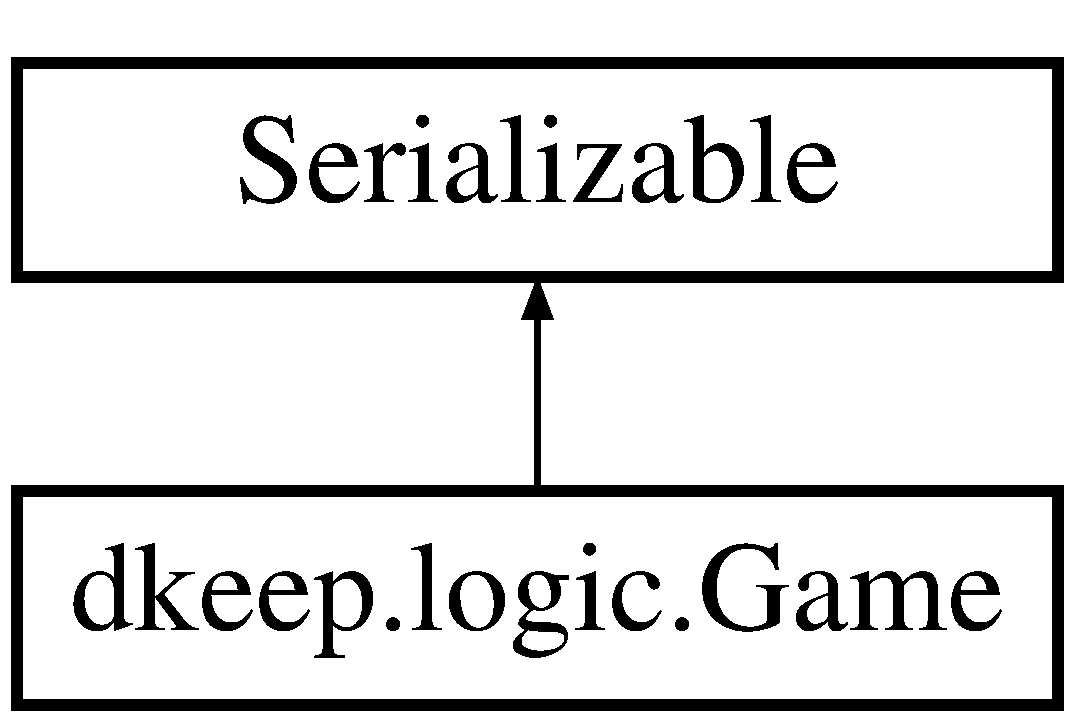
\includegraphics[height=2.000000cm]{classdkeep_1_1logic_1_1_game}
\end{center}
\end{figure}
\subsection*{Public Member Functions}
\begin{DoxyCompactItemize}
\item 
\hyperlink{classdkeep_1_1logic_1_1_game_ad630e9f66ca2e6fc818411499b9a7d7a}{Game} (\hyperlink{classdkeep_1_1logic_1_1_map}{Map} starting\+Map, \hyperlink{classdkeep_1_1logic_1_1_logic}{Logic} starting\+Logic, int\mbox{[}$\,$\mbox{]} num\+Enemy)
\item 
boolean \hyperlink{classdkeep_1_1logic_1_1_game_a6f548ad7f01432adb418f5891f130ec4}{is\+Game\+Over} ()
\item 
boolean \hyperlink{classdkeep_1_1logic_1_1_game_af2953cb36d8db8ff068d0291f6c6dbba}{victory} ()
\item 
void \hyperlink{classdkeep_1_1logic_1_1_game_a45d8230123f2046b5d5a82ba7e6b2147}{get\+Board\+Key} (char\mbox{[}$\,$\mbox{]}\mbox{[}$\,$\mbox{]} m)
\item 
void \hyperlink{classdkeep_1_1logic_1_1_game_a5a87ac790c4389d6e6066e19e4be4983}{erase\+Board\+Key} (char\mbox{[}$\,$\mbox{]}\mbox{[}$\,$\mbox{]} m)
\item 
void \hyperlink{classdkeep_1_1logic_1_1_game_a4d9a18b2ade5e68657a41d2f2516f696}{get\+Board\+Hero} (char\mbox{[}$\,$\mbox{]}\mbox{[}$\,$\mbox{]} m)
\item 
void \hyperlink{classdkeep_1_1logic_1_1_game_afe09f2713bb62e5ace6943edb3306043}{erase\+Board\+Hero} (char\mbox{[}$\,$\mbox{]}\mbox{[}$\,$\mbox{]} m)
\item 
void \hyperlink{classdkeep_1_1logic_1_1_game_a891c0dd84b0a828714135cf2e56258e8}{get\+Board\+Enemies} (char\mbox{[}$\,$\mbox{]}\mbox{[}$\,$\mbox{]} m)
\item 
void \hyperlink{classdkeep_1_1logic_1_1_game_acb0bd46f08b7987f30692afcc49525cf}{erase\+Board\+Enemies} (char\mbox{[}$\,$\mbox{]}\mbox{[}$\,$\mbox{]} m)
\item 
char \mbox{[}$\,$\mbox{]}\mbox{[}$\,$\mbox{]} \hyperlink{classdkeep_1_1logic_1_1_game_a00104638b06a79e0b90768a1df2628c2}{get\+Board} ()
\item 
int \hyperlink{classdkeep_1_1logic_1_1_game_ada3e80740d47374027077803c6442ca4}{get\+Level} ()
\item 
void \hyperlink{classdkeep_1_1logic_1_1_game_af80ce295e13bccbe8fe6f48399d4d808}{set\+Level} (int level)
\item 
void \hyperlink{classdkeep_1_1logic_1_1_game_a10736bc5627d884177a850b7b3182fb4}{move\+Hero} (char dir)
\item 
void \hyperlink{classdkeep_1_1logic_1_1_game_add0b32fc7d2370e0071ccdf85ee341e1}{update} (char dir)
\end{DoxyCompactItemize}


\subsection{Detailed Description}
\hyperlink{classdkeep_1_1logic_1_1_game}{Game} is a class that deals with the whole game, connecting logics with the respective map. This class checks if the game is over and either proceeds to the next level (if there is one), or ends the game and transmits that information to the main function. It contains the map and logic of the game, the enemy\textquotesingle{}s options of each level and the current level of the game being played. 

\subsection{Constructor \& Destructor Documentation}
\mbox{\Hypertarget{classdkeep_1_1logic_1_1_game_ad630e9f66ca2e6fc818411499b9a7d7a}\label{classdkeep_1_1logic_1_1_game_ad630e9f66ca2e6fc818411499b9a7d7a}} 
\index{dkeep\+::logic\+::\+Game@{dkeep\+::logic\+::\+Game}!Game@{Game}}
\index{Game@{Game}!dkeep\+::logic\+::\+Game@{dkeep\+::logic\+::\+Game}}
\subsubsection{\texorpdfstring{Game()}{Game()}}
{\footnotesize\ttfamily dkeep.\+logic.\+Game.\+Game (\begin{DoxyParamCaption}\item[{\hyperlink{classdkeep_1_1logic_1_1_map}{Map}}]{starting\+Map,  }\item[{\hyperlink{classdkeep_1_1logic_1_1_logic}{Logic}}]{starting\+Logic,  }\item[{int \mbox{[}$\,$\mbox{]}}]{num\+Enemy }\end{DoxyParamCaption})}

Constructor of \hyperlink{classdkeep_1_1logic_1_1_game}{Game}. Initializes the map, logic and enemyoptions with the attributes given and sets the level to 0. 
\begin{DoxyParams}{Parameters}
{\em starting\+Map} & \hyperlink{classdkeep_1_1logic_1_1_map}{Map} that is playable in the beginning of the game \\
\hline
{\em starting\+Logic} & \hyperlink{classdkeep_1_1logic_1_1_logic}{Logic} that is playable in the beginning of the game \\
\hline
{\em num\+Enemy} & Options regarding the enemies of the existing levels \\
\hline
\end{DoxyParams}


\subsection{Member Function Documentation}
\mbox{\Hypertarget{classdkeep_1_1logic_1_1_game_acb0bd46f08b7987f30692afcc49525cf}\label{classdkeep_1_1logic_1_1_game_acb0bd46f08b7987f30692afcc49525cf}} 
\index{dkeep\+::logic\+::\+Game@{dkeep\+::logic\+::\+Game}!erase\+Board\+Enemies@{erase\+Board\+Enemies}}
\index{erase\+Board\+Enemies@{erase\+Board\+Enemies}!dkeep\+::logic\+::\+Game@{dkeep\+::logic\+::\+Game}}
\subsubsection{\texorpdfstring{erase\+Board\+Enemies()}{eraseBoardEnemies()}}
{\footnotesize\ttfamily void dkeep.\+logic.\+Game.\+erase\+Board\+Enemies (\begin{DoxyParamCaption}\item[{char}]{m\mbox{[}$\,$\mbox{]}\mbox{[}$\,$\mbox{]} }\end{DoxyParamCaption})}

Erases from the map the enemies symbol and their weapon. 
\begin{DoxyParams}{Parameters}
{\em m} & matrix of chars that represent the map of the game \\
\hline
\end{DoxyParams}
\mbox{\Hypertarget{classdkeep_1_1logic_1_1_game_afe09f2713bb62e5ace6943edb3306043}\label{classdkeep_1_1logic_1_1_game_afe09f2713bb62e5ace6943edb3306043}} 
\index{dkeep\+::logic\+::\+Game@{dkeep\+::logic\+::\+Game}!erase\+Board\+Hero@{erase\+Board\+Hero}}
\index{erase\+Board\+Hero@{erase\+Board\+Hero}!dkeep\+::logic\+::\+Game@{dkeep\+::logic\+::\+Game}}
\subsubsection{\texorpdfstring{erase\+Board\+Hero()}{eraseBoardHero()}}
{\footnotesize\ttfamily void dkeep.\+logic.\+Game.\+erase\+Board\+Hero (\begin{DoxyParamCaption}\item[{char}]{m\mbox{[}$\,$\mbox{]}\mbox{[}$\,$\mbox{]} }\end{DoxyParamCaption})}

Erases from the map the hero symbol and its weapon. 
\begin{DoxyParams}{Parameters}
{\em m} & matrix of chars that represent the map of the game \\
\hline
\end{DoxyParams}
\mbox{\Hypertarget{classdkeep_1_1logic_1_1_game_a5a87ac790c4389d6e6066e19e4be4983}\label{classdkeep_1_1logic_1_1_game_a5a87ac790c4389d6e6066e19e4be4983}} 
\index{dkeep\+::logic\+::\+Game@{dkeep\+::logic\+::\+Game}!erase\+Board\+Key@{erase\+Board\+Key}}
\index{erase\+Board\+Key@{erase\+Board\+Key}!dkeep\+::logic\+::\+Game@{dkeep\+::logic\+::\+Game}}
\subsubsection{\texorpdfstring{erase\+Board\+Key()}{eraseBoardKey()}}
{\footnotesize\ttfamily void dkeep.\+logic.\+Game.\+erase\+Board\+Key (\begin{DoxyParamCaption}\item[{char}]{m\mbox{[}$\,$\mbox{]}\mbox{[}$\,$\mbox{]} }\end{DoxyParamCaption})}

Erases from the map the key symbol. 
\begin{DoxyParams}{Parameters}
{\em m} & matrix of chars that represent the map of the game \\
\hline
\end{DoxyParams}
\mbox{\Hypertarget{classdkeep_1_1logic_1_1_game_a00104638b06a79e0b90768a1df2628c2}\label{classdkeep_1_1logic_1_1_game_a00104638b06a79e0b90768a1df2628c2}} 
\index{dkeep\+::logic\+::\+Game@{dkeep\+::logic\+::\+Game}!get\+Board@{get\+Board}}
\index{get\+Board@{get\+Board}!dkeep\+::logic\+::\+Game@{dkeep\+::logic\+::\+Game}}
\subsubsection{\texorpdfstring{get\+Board()}{getBoard()}}
{\footnotesize\ttfamily char \mbox{[}$\,$\mbox{]}\mbox{[}$\,$\mbox{]} dkeep.\+logic.\+Game.\+get\+Board (\begin{DoxyParamCaption}{ }\end{DoxyParamCaption})}

Puts all the non-\/static elements of the game on the map, saves it into a matrix of chars and also prints it. In the end, erases all the non-\/static elements. \begin{DoxyReturn}{Returns}
matrix of chars that contain the current map of the game 
\end{DoxyReturn}
\mbox{\Hypertarget{classdkeep_1_1logic_1_1_game_a891c0dd84b0a828714135cf2e56258e8}\label{classdkeep_1_1logic_1_1_game_a891c0dd84b0a828714135cf2e56258e8}} 
\index{dkeep\+::logic\+::\+Game@{dkeep\+::logic\+::\+Game}!get\+Board\+Enemies@{get\+Board\+Enemies}}
\index{get\+Board\+Enemies@{get\+Board\+Enemies}!dkeep\+::logic\+::\+Game@{dkeep\+::logic\+::\+Game}}
\subsubsection{\texorpdfstring{get\+Board\+Enemies()}{getBoardEnemies()}}
{\footnotesize\ttfamily void dkeep.\+logic.\+Game.\+get\+Board\+Enemies (\begin{DoxyParamCaption}\item[{char}]{m\mbox{[}$\,$\mbox{]}\mbox{[}$\,$\mbox{]} }\end{DoxyParamCaption})}

Prints in the map the enemies symbol and their weapon, in their current position. 
\begin{DoxyParams}{Parameters}
{\em m} & matrix of chars that represent the map of the game \\
\hline
\end{DoxyParams}
\mbox{\Hypertarget{classdkeep_1_1logic_1_1_game_a4d9a18b2ade5e68657a41d2f2516f696}\label{classdkeep_1_1logic_1_1_game_a4d9a18b2ade5e68657a41d2f2516f696}} 
\index{dkeep\+::logic\+::\+Game@{dkeep\+::logic\+::\+Game}!get\+Board\+Hero@{get\+Board\+Hero}}
\index{get\+Board\+Hero@{get\+Board\+Hero}!dkeep\+::logic\+::\+Game@{dkeep\+::logic\+::\+Game}}
\subsubsection{\texorpdfstring{get\+Board\+Hero()}{getBoardHero()}}
{\footnotesize\ttfamily void dkeep.\+logic.\+Game.\+get\+Board\+Hero (\begin{DoxyParamCaption}\item[{char}]{m\mbox{[}$\,$\mbox{]}\mbox{[}$\,$\mbox{]} }\end{DoxyParamCaption})}

Prints in the map the hero symbol and its weapon in their current position. 
\begin{DoxyParams}{Parameters}
{\em m} & matrix of chars that represent the map of the game \\
\hline
\end{DoxyParams}
\mbox{\Hypertarget{classdkeep_1_1logic_1_1_game_a45d8230123f2046b5d5a82ba7e6b2147}\label{classdkeep_1_1logic_1_1_game_a45d8230123f2046b5d5a82ba7e6b2147}} 
\index{dkeep\+::logic\+::\+Game@{dkeep\+::logic\+::\+Game}!get\+Board\+Key@{get\+Board\+Key}}
\index{get\+Board\+Key@{get\+Board\+Key}!dkeep\+::logic\+::\+Game@{dkeep\+::logic\+::\+Game}}
\subsubsection{\texorpdfstring{get\+Board\+Key()}{getBoardKey()}}
{\footnotesize\ttfamily void dkeep.\+logic.\+Game.\+get\+Board\+Key (\begin{DoxyParamCaption}\item[{char}]{m\mbox{[}$\,$\mbox{]}\mbox{[}$\,$\mbox{]} }\end{DoxyParamCaption})}

Prints in the map the key symbol in it\textquotesingle{}s current position. 
\begin{DoxyParams}{Parameters}
{\em m} & matrix of chars that represent the map of the game \\
\hline
\end{DoxyParams}
\mbox{\Hypertarget{classdkeep_1_1logic_1_1_game_ada3e80740d47374027077803c6442ca4}\label{classdkeep_1_1logic_1_1_game_ada3e80740d47374027077803c6442ca4}} 
\index{dkeep\+::logic\+::\+Game@{dkeep\+::logic\+::\+Game}!get\+Level@{get\+Level}}
\index{get\+Level@{get\+Level}!dkeep\+::logic\+::\+Game@{dkeep\+::logic\+::\+Game}}
\subsubsection{\texorpdfstring{get\+Level()}{getLevel()}}
{\footnotesize\ttfamily int dkeep.\+logic.\+Game.\+get\+Level (\begin{DoxyParamCaption}{ }\end{DoxyParamCaption})}

Returns the current level of the game. \begin{DoxyReturn}{Returns}
level attribute 
\end{DoxyReturn}
\mbox{\Hypertarget{classdkeep_1_1logic_1_1_game_a6f548ad7f01432adb418f5891f130ec4}\label{classdkeep_1_1logic_1_1_game_a6f548ad7f01432adb418f5891f130ec4}} 
\index{dkeep\+::logic\+::\+Game@{dkeep\+::logic\+::\+Game}!is\+Game\+Over@{is\+Game\+Over}}
\index{is\+Game\+Over@{is\+Game\+Over}!dkeep\+::logic\+::\+Game@{dkeep\+::logic\+::\+Game}}
\subsubsection{\texorpdfstring{is\+Game\+Over()}{isGameOver()}}
{\footnotesize\ttfamily boolean dkeep.\+logic.\+Game.\+is\+Game\+Over (\begin{DoxyParamCaption}{ }\end{DoxyParamCaption})}

Checks with the logic to see if the game in the level is over, return true if it is, false if not. \begin{DoxyReturn}{Returns}
true if the level is over, false if not 
\end{DoxyReturn}
\mbox{\Hypertarget{classdkeep_1_1logic_1_1_game_a10736bc5627d884177a850b7b3182fb4}\label{classdkeep_1_1logic_1_1_game_a10736bc5627d884177a850b7b3182fb4}} 
\index{dkeep\+::logic\+::\+Game@{dkeep\+::logic\+::\+Game}!move\+Hero@{move\+Hero}}
\index{move\+Hero@{move\+Hero}!dkeep\+::logic\+::\+Game@{dkeep\+::logic\+::\+Game}}
\subsubsection{\texorpdfstring{move\+Hero()}{moveHero()}}
{\footnotesize\ttfamily void dkeep.\+logic.\+Game.\+move\+Hero (\begin{DoxyParamCaption}\item[{char}]{dir }\end{DoxyParamCaption})}

Moves the hero in the direction chosen by the player. 
\begin{DoxyParams}{Parameters}
{\em dir} & direction to which move the hero \\
\hline
\end{DoxyParams}
\mbox{\Hypertarget{classdkeep_1_1logic_1_1_game_af80ce295e13bccbe8fe6f48399d4d808}\label{classdkeep_1_1logic_1_1_game_af80ce295e13bccbe8fe6f48399d4d808}} 
\index{dkeep\+::logic\+::\+Game@{dkeep\+::logic\+::\+Game}!set\+Level@{set\+Level}}
\index{set\+Level@{set\+Level}!dkeep\+::logic\+::\+Game@{dkeep\+::logic\+::\+Game}}
\subsubsection{\texorpdfstring{set\+Level()}{setLevel()}}
{\footnotesize\ttfamily void dkeep.\+logic.\+Game.\+set\+Level (\begin{DoxyParamCaption}\item[{int}]{level }\end{DoxyParamCaption})}

Sets the level attribute to a new value. 
\begin{DoxyParams}{Parameters}
{\em level} & new value of level \\
\hline
\end{DoxyParams}
\mbox{\Hypertarget{classdkeep_1_1logic_1_1_game_add0b32fc7d2370e0071ccdf85ee341e1}\label{classdkeep_1_1logic_1_1_game_add0b32fc7d2370e0071ccdf85ee341e1}} 
\index{dkeep\+::logic\+::\+Game@{dkeep\+::logic\+::\+Game}!update@{update}}
\index{update@{update}!dkeep\+::logic\+::\+Game@{dkeep\+::logic\+::\+Game}}
\subsubsection{\texorpdfstring{update()}{update()}}
{\footnotesize\ttfamily void dkeep.\+logic.\+Game.\+update (\begin{DoxyParamCaption}\item[{char}]{dir }\end{DoxyParamCaption})}

Updates the state of the game and checks if it ended in victory. If that is case and there is a next level, it requests the logic and map of the next level. 
\begin{DoxyParams}{Parameters}
{\em dir} & direction to which move the hero \\
\hline
\end{DoxyParams}
\mbox{\Hypertarget{classdkeep_1_1logic_1_1_game_af2953cb36d8db8ff068d0291f6c6dbba}\label{classdkeep_1_1logic_1_1_game_af2953cb36d8db8ff068d0291f6c6dbba}} 
\index{dkeep\+::logic\+::\+Game@{dkeep\+::logic\+::\+Game}!victory@{victory}}
\index{victory@{victory}!dkeep\+::logic\+::\+Game@{dkeep\+::logic\+::\+Game}}
\subsubsection{\texorpdfstring{victory()}{victory()}}
{\footnotesize\ttfamily boolean dkeep.\+logic.\+Game.\+victory (\begin{DoxyParamCaption}{ }\end{DoxyParamCaption})}

Checks with the logic to see if the game in the level ended in victory, return true if it has, false if not. \begin{DoxyReturn}{Returns}
true if the level ended in victory, false if not 
\end{DoxyReturn}


The documentation for this class was generated from the following file\+:\begin{DoxyCompactItemize}
\item 
C\+:/\+Users/\+M\+C-\/\+Guida/git/\+L\+P\+O\+O1617\+\_\+\+T1\+G5/\+Lab05/src/dkeep/logic/Game.\+java\end{DoxyCompactItemize}

\hypertarget{classdkeep_1_1logic_1_1_guard}{}\section{dkeep.\+logic.\+Guard Class Reference}
\label{classdkeep_1_1logic_1_1_guard}\index{dkeep.\+logic.\+Guard@{dkeep.\+logic.\+Guard}}
Inheritance diagram for dkeep.\+logic.\+Guard\+:\begin{figure}[H]
\begin{center}
\leavevmode
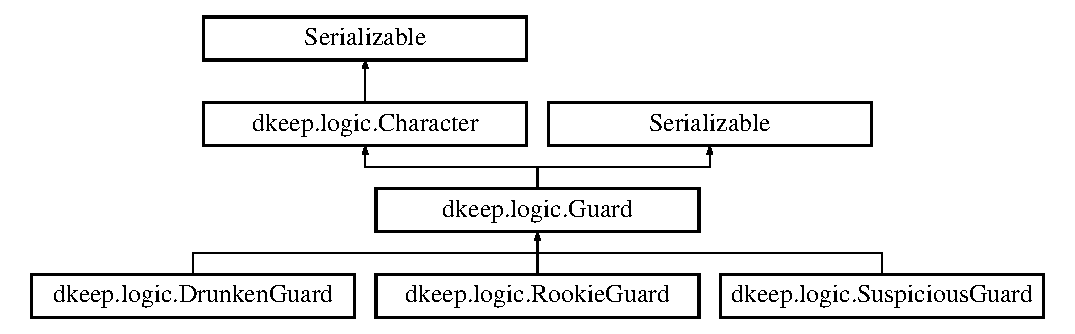
\includegraphics[height=4.000000cm]{classdkeep_1_1logic_1_1_guard}
\end{center}
\end{figure}
\subsection*{Public Member Functions}
\begin{DoxyCompactItemize}
\item 
\hyperlink{classdkeep_1_1logic_1_1_guard_a3e09758314f42000eca6134717672855}{Guard} (char symbol, int\mbox{[}$\,$\mbox{]} coord, char\mbox{[}$\,$\mbox{]} path)
\item 
int \mbox{[}$\,$\mbox{]} \hyperlink{classdkeep_1_1logic_1_1_guard_a2389016085c6d65d4366930fac72dab4}{normal\+Movement} ()
\item 
int \mbox{[}$\,$\mbox{]} \hyperlink{classdkeep_1_1logic_1_1_guard_a8c588aa887fcfe6d3e4a9e13d236c644}{reverse\+Movement} ()
\item 
int \mbox{[}$\,$\mbox{]} \hyperlink{classdkeep_1_1logic_1_1_guard_a4c4590d86f573a575bc3ece3d441f83f}{movement} ()
\item 
char \hyperlink{classdkeep_1_1logic_1_1_guard_a2008fdc91b313fa18059fab7d92ddc61}{get\+Symbol} ()
\end{DoxyCompactItemize}
\subsection*{Protected Attributes}
\begin{DoxyCompactItemize}
\item 
\mbox{\Hypertarget{classdkeep_1_1logic_1_1_guard_a74ea55aa131d73784e9487ef3aeef5ca}\label{classdkeep_1_1logic_1_1_guard_a74ea55aa131d73784e9487ef3aeef5ca}} 
char \mbox{[}$\,$\mbox{]} {\bfseries path}
\item 
\mbox{\Hypertarget{classdkeep_1_1logic_1_1_guard_a0e0434321ead6cd193358d9069177ba3}\label{classdkeep_1_1logic_1_1_guard_a0e0434321ead6cd193358d9069177ba3}} 
int {\bfseries i}
\end{DoxyCompactItemize}


\subsection{Detailed Description}
\hyperlink{classdkeep_1_1logic_1_1_guard}{Guard} is a class that keeps information about the type of enemy \hyperlink{classdkeep_1_1logic_1_1_guard}{Guard}. This information consists of the path corresponding to it\textquotesingle{}s movement on the map and the index that keeps track of that path. It also contains the methods for the normal movement (following the path) and the reverse movement(following the path in reverse order). \begin{DoxySeeAlso}{See also}
\hyperlink{classdkeep_1_1logic_1_1_character}{Character} 
\end{DoxySeeAlso}


\subsection{Constructor \& Destructor Documentation}
\mbox{\Hypertarget{classdkeep_1_1logic_1_1_guard_a3e09758314f42000eca6134717672855}\label{classdkeep_1_1logic_1_1_guard_a3e09758314f42000eca6134717672855}} 
\index{dkeep\+::logic\+::\+Guard@{dkeep\+::logic\+::\+Guard}!Guard@{Guard}}
\index{Guard@{Guard}!dkeep\+::logic\+::\+Guard@{dkeep\+::logic\+::\+Guard}}
\subsubsection{\texorpdfstring{Guard()}{Guard()}}
{\footnotesize\ttfamily dkeep.\+logic.\+Guard.\+Guard (\begin{DoxyParamCaption}\item[{char}]{symbol,  }\item[{int \mbox{[}$\,$\mbox{]}}]{coord,  }\item[{char \mbox{[}$\,$\mbox{]}}]{path }\end{DoxyParamCaption})}

Constructor of \hyperlink{classdkeep_1_1logic_1_1_guard}{Guard}. It initializes the character variables and also the path and index. 
\begin{DoxyParams}{Parameters}
{\em symbol} & char that represents the guard \\
\hline
{\em x} & coordinate \\
\hline
{\em y} & coordinate \\
\hline
{\em path} & array of chars that represent the path that the enemy will take \\
\hline
{\em i} & int that keeps the progress in the array of path \\
\hline
\end{DoxyParams}


\subsection{Member Function Documentation}
\mbox{\Hypertarget{classdkeep_1_1logic_1_1_guard_a2008fdc91b313fa18059fab7d92ddc61}\label{classdkeep_1_1logic_1_1_guard_a2008fdc91b313fa18059fab7d92ddc61}} 
\index{dkeep\+::logic\+::\+Guard@{dkeep\+::logic\+::\+Guard}!get\+Symbol@{get\+Symbol}}
\index{get\+Symbol@{get\+Symbol}!dkeep\+::logic\+::\+Guard@{dkeep\+::logic\+::\+Guard}}
\subsubsection{\texorpdfstring{get\+Symbol()}{getSymbol()}}
{\footnotesize\ttfamily char dkeep.\+logic.\+Guard.\+get\+Symbol (\begin{DoxyParamCaption}{ }\end{DoxyParamCaption})}

\mbox{\Hypertarget{classdkeep_1_1logic_1_1_guard_a4c4590d86f573a575bc3ece3d441f83f}\label{classdkeep_1_1logic_1_1_guard_a4c4590d86f573a575bc3ece3d441f83f}} 
\index{dkeep\+::logic\+::\+Guard@{dkeep\+::logic\+::\+Guard}!movement@{movement}}
\index{movement@{movement}!dkeep\+::logic\+::\+Guard@{dkeep\+::logic\+::\+Guard}}
\subsubsection{\texorpdfstring{movement()}{movement()}}
{\footnotesize\ttfamily int \mbox{[}$\,$\mbox{]} dkeep.\+logic.\+Guard.\+movement (\begin{DoxyParamCaption}{ }\end{DoxyParamCaption})}

\mbox{\Hypertarget{classdkeep_1_1logic_1_1_guard_a2389016085c6d65d4366930fac72dab4}\label{classdkeep_1_1logic_1_1_guard_a2389016085c6d65d4366930fac72dab4}} 
\index{dkeep\+::logic\+::\+Guard@{dkeep\+::logic\+::\+Guard}!normal\+Movement@{normal\+Movement}}
\index{normal\+Movement@{normal\+Movement}!dkeep\+::logic\+::\+Guard@{dkeep\+::logic\+::\+Guard}}
\subsubsection{\texorpdfstring{normal\+Movement()}{normalMovement()}}
{\footnotesize\ttfamily int \mbox{[}$\,$\mbox{]} dkeep.\+logic.\+Guard.\+normal\+Movement (\begin{DoxyParamCaption}{ }\end{DoxyParamCaption})}

Follows the path of the guard, using the index to know the next direction of the guard. Returns a array with the new coordinates of the guard and updates the index. \begin{DoxyReturn}{Returns}
array of 2 ints with the coordinates x and y 
\end{DoxyReturn}
\mbox{\Hypertarget{classdkeep_1_1logic_1_1_guard_a8c588aa887fcfe6d3e4a9e13d236c644}\label{classdkeep_1_1logic_1_1_guard_a8c588aa887fcfe6d3e4a9e13d236c644}} 
\index{dkeep\+::logic\+::\+Guard@{dkeep\+::logic\+::\+Guard}!reverse\+Movement@{reverse\+Movement}}
\index{reverse\+Movement@{reverse\+Movement}!dkeep\+::logic\+::\+Guard@{dkeep\+::logic\+::\+Guard}}
\subsubsection{\texorpdfstring{reverse\+Movement()}{reverseMovement()}}
{\footnotesize\ttfamily int \mbox{[}$\,$\mbox{]} dkeep.\+logic.\+Guard.\+reverse\+Movement (\begin{DoxyParamCaption}{ }\end{DoxyParamCaption})}

Follows the path of the guard but in reverse order. Instead of adding 1 to the index, it subtracts 1. Returns a array with the new coordinates of the guard.

\begin{DoxyReturn}{Returns}
array of 2 ints with the coordinates x and y 
\end{DoxyReturn}


The documentation for this class was generated from the following file\+:\begin{DoxyCompactItemize}
\item 
C\+:/\+Users/\+M\+C-\/\+Guida/git/\+L\+P\+O\+O1617\+\_\+\+T1\+G5/\+Lab05/src/dkeep/logic/Guard.\+java\end{DoxyCompactItemize}

\hypertarget{classdkeep_1_1logic_1_1_hero}{}\section{dkeep.\+logic.\+Hero Class Reference}
\label{classdkeep_1_1logic_1_1_hero}\index{dkeep.\+logic.\+Hero@{dkeep.\+logic.\+Hero}}
Inheritance diagram for dkeep.\+logic.\+Hero\+:\begin{figure}[H]
\begin{center}
\leavevmode
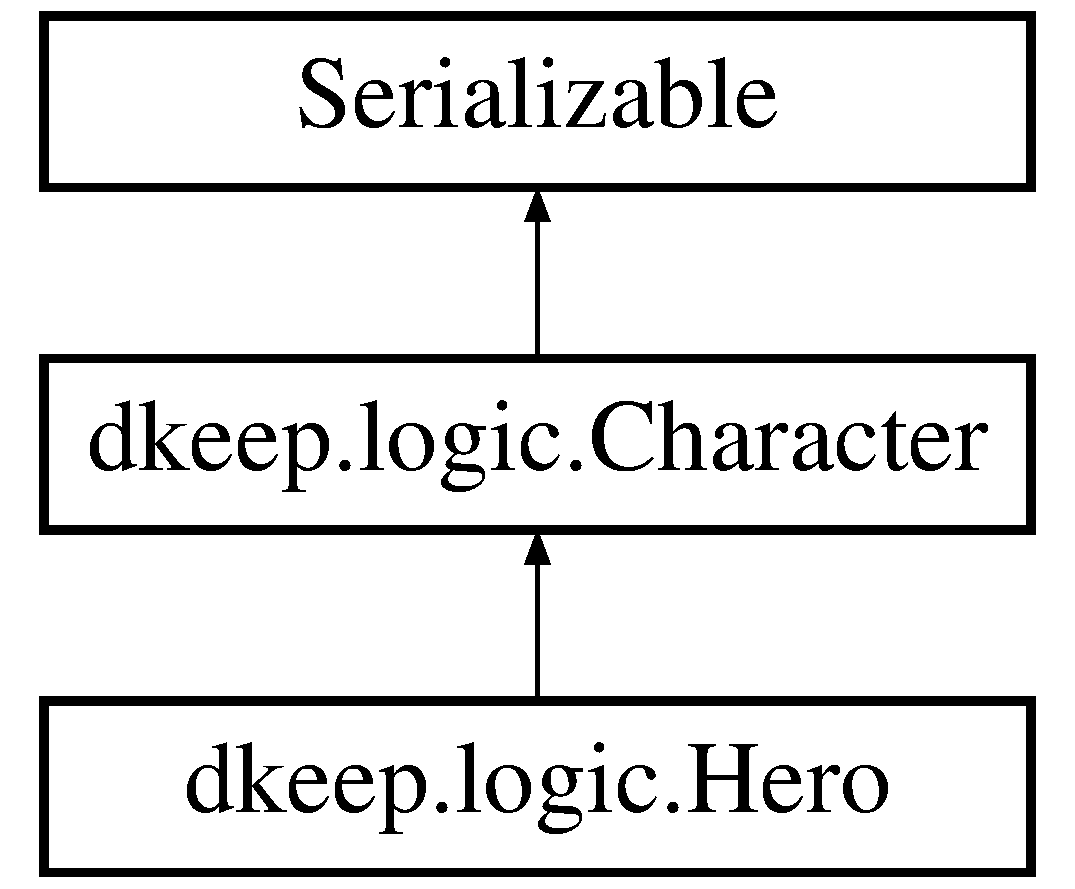
\includegraphics[height=3.000000cm]{classdkeep_1_1logic_1_1_hero}
\end{center}
\end{figure}
\subsection*{Public Member Functions}
\begin{DoxyCompactItemize}
\item 
\hyperlink{classdkeep_1_1logic_1_1_hero_ae74a6e3427b1da89bd52b14cdc632d9b}{Hero} (char s, int\mbox{[}$\,$\mbox{]} coord, \hyperlink{classdkeep_1_1logic_1_1_weapon}{Weapon} weapon)
\item 
void \hyperlink{classdkeep_1_1logic_1_1_hero_a5fb6abc6ce91464833c67f143b4f913b}{set\+Dir} (char dir)
\item 
int \mbox{[}$\,$\mbox{]} \hyperlink{classdkeep_1_1logic_1_1_hero_a5c9eff750321d53e1e4257fd9efd4cd6}{movement} ()
\item 
boolean \hyperlink{classdkeep_1_1logic_1_1_hero_a5fc18a0a10613780cdc6b966dc8810f1}{has\+Key} ()
\item 
void \hyperlink{classdkeep_1_1logic_1_1_hero_a72b13a616bd52ce76b73e6e5e96ccf72}{set\+Key\+True} ()
\item 
char \hyperlink{classdkeep_1_1logic_1_1_hero_afaf5e4c05717a5bdf568c565339e30f6}{get\+Symbol} ()
\end{DoxyCompactItemize}
\subsection*{Additional Inherited Members}


\subsection{Detailed Description}
\hyperlink{classdkeep_1_1logic_1_1_hero}{Hero} is a class that represents the hero of the game, that is, the character controlled by the user. \begin{DoxySeeAlso}{See also}
\hyperlink{classdkeep_1_1logic_1_1_character}{Character} 
\end{DoxySeeAlso}


\subsection{Constructor \& Destructor Documentation}
\mbox{\Hypertarget{classdkeep_1_1logic_1_1_hero_ae74a6e3427b1da89bd52b14cdc632d9b}\label{classdkeep_1_1logic_1_1_hero_ae74a6e3427b1da89bd52b14cdc632d9b}} 
\index{dkeep\+::logic\+::\+Hero@{dkeep\+::logic\+::\+Hero}!Hero@{Hero}}
\index{Hero@{Hero}!dkeep\+::logic\+::\+Hero@{dkeep\+::logic\+::\+Hero}}
\subsubsection{\texorpdfstring{Hero()}{Hero()}}
{\footnotesize\ttfamily dkeep.\+logic.\+Hero.\+Hero (\begin{DoxyParamCaption}\item[{char}]{s,  }\item[{int \mbox{[}$\,$\mbox{]}}]{coord,  }\item[{\hyperlink{classdkeep_1_1logic_1_1_weapon}{Weapon}}]{weapon }\end{DoxyParamCaption})}

Constructor of \hyperlink{classdkeep_1_1logic_1_1_hero}{Hero}. Puts all flags to false and initialize all elements with the information given. The weapon can be null. 
\begin{DoxyParams}{Parameters}
{\em s} & char that represents the hero \\
\hline
{\em x} & coordinate \\
\hline
{\em y} & coordinate \\
\hline
{\em weapon} & object \hyperlink{classdkeep_1_1logic_1_1_weapon}{Weapon} that contains information about a \hyperlink{classdkeep_1_1logic_1_1_club}{Club} \\
\hline
\end{DoxyParams}


\subsection{Member Function Documentation}
\mbox{\Hypertarget{classdkeep_1_1logic_1_1_hero_afaf5e4c05717a5bdf568c565339e30f6}\label{classdkeep_1_1logic_1_1_hero_afaf5e4c05717a5bdf568c565339e30f6}} 
\index{dkeep\+::logic\+::\+Hero@{dkeep\+::logic\+::\+Hero}!get\+Symbol@{get\+Symbol}}
\index{get\+Symbol@{get\+Symbol}!dkeep\+::logic\+::\+Hero@{dkeep\+::logic\+::\+Hero}}
\subsubsection{\texorpdfstring{get\+Symbol()}{getSymbol()}}
{\footnotesize\ttfamily char dkeep.\+logic.\+Hero.\+get\+Symbol (\begin{DoxyParamCaption}{ }\end{DoxyParamCaption})}

In this specific class, if the hero has caught the key, the symbol will be different. \mbox{\Hypertarget{classdkeep_1_1logic_1_1_hero_a5fc18a0a10613780cdc6b966dc8810f1}\label{classdkeep_1_1logic_1_1_hero_a5fc18a0a10613780cdc6b966dc8810f1}} 
\index{dkeep\+::logic\+::\+Hero@{dkeep\+::logic\+::\+Hero}!has\+Key@{has\+Key}}
\index{has\+Key@{has\+Key}!dkeep\+::logic\+::\+Hero@{dkeep\+::logic\+::\+Hero}}
\subsubsection{\texorpdfstring{has\+Key()}{hasKey()}}
{\footnotesize\ttfamily boolean dkeep.\+logic.\+Hero.\+has\+Key (\begin{DoxyParamCaption}{ }\end{DoxyParamCaption})}

Returns boolean corresponding to the hero\textquotesingle{}s possession of the key. \begin{DoxyReturn}{Returns}
true if the hero has the key, false if not 
\end{DoxyReturn}
\mbox{\Hypertarget{classdkeep_1_1logic_1_1_hero_a5c9eff750321d53e1e4257fd9efd4cd6}\label{classdkeep_1_1logic_1_1_hero_a5c9eff750321d53e1e4257fd9efd4cd6}} 
\index{dkeep\+::logic\+::\+Hero@{dkeep\+::logic\+::\+Hero}!movement@{movement}}
\index{movement@{movement}!dkeep\+::logic\+::\+Hero@{dkeep\+::logic\+::\+Hero}}
\subsubsection{\texorpdfstring{movement()}{movement()}}
{\footnotesize\ttfamily int \mbox{[}$\,$\mbox{]} dkeep.\+logic.\+Hero.\+movement (\begin{DoxyParamCaption}{ }\end{DoxyParamCaption})}

\mbox{\Hypertarget{classdkeep_1_1logic_1_1_hero_a5fb6abc6ce91464833c67f143b4f913b}\label{classdkeep_1_1logic_1_1_hero_a5fb6abc6ce91464833c67f143b4f913b}} 
\index{dkeep\+::logic\+::\+Hero@{dkeep\+::logic\+::\+Hero}!set\+Dir@{set\+Dir}}
\index{set\+Dir@{set\+Dir}!dkeep\+::logic\+::\+Hero@{dkeep\+::logic\+::\+Hero}}
\subsubsection{\texorpdfstring{set\+Dir()}{setDir()}}
{\footnotesize\ttfamily void dkeep.\+logic.\+Hero.\+set\+Dir (\begin{DoxyParamCaption}\item[{char}]{dir }\end{DoxyParamCaption})}

Sets the direction of the hero to a particular direction (a -\/ left, d -\/ right, w -\/ up, s -\/ down). 
\begin{DoxyParams}{Parameters}
{\em dir} & movement direction taken by the hero \\
\hline
\end{DoxyParams}
\mbox{\Hypertarget{classdkeep_1_1logic_1_1_hero_a72b13a616bd52ce76b73e6e5e96ccf72}\label{classdkeep_1_1logic_1_1_hero_a72b13a616bd52ce76b73e6e5e96ccf72}} 
\index{dkeep\+::logic\+::\+Hero@{dkeep\+::logic\+::\+Hero}!set\+Key\+True@{set\+Key\+True}}
\index{set\+Key\+True@{set\+Key\+True}!dkeep\+::logic\+::\+Hero@{dkeep\+::logic\+::\+Hero}}
\subsubsection{\texorpdfstring{set\+Key\+True()}{setKeyTrue()}}
{\footnotesize\ttfamily void dkeep.\+logic.\+Hero.\+set\+Key\+True (\begin{DoxyParamCaption}{ }\end{DoxyParamCaption})}

Sets true the has\+Key flag, meaning that the hero has caught the key. 

The documentation for this class was generated from the following file\+:\begin{DoxyCompactItemize}
\item 
C\+:/\+Users/\+M\+C-\/\+Guida/git/\+L\+P\+O\+O1617\+\_\+\+T1\+G5/\+Lab05/src/dkeep/logic/Hero.\+java\end{DoxyCompactItemize}

\hypertarget{classdkeep_1_1logic_1_1_keep_logic}{}\section{dkeep.\+logic.\+Keep\+Logic Class Reference}
\label{classdkeep_1_1logic_1_1_keep_logic}\index{dkeep.\+logic.\+Keep\+Logic@{dkeep.\+logic.\+Keep\+Logic}}
Inheritance diagram for dkeep.\+logic.\+Keep\+Logic\+:\begin{figure}[H]
\begin{center}
\leavevmode
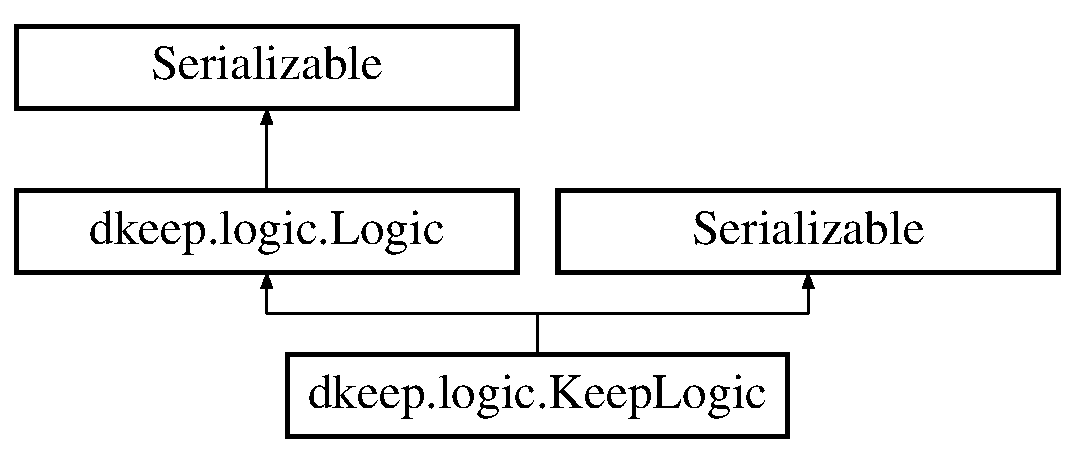
\includegraphics[height=3.000000cm]{classdkeep_1_1logic_1_1_keep_logic}
\end{center}
\end{figure}
\subsection*{Public Member Functions}
\begin{DoxyCompactItemize}
\item 
\hyperlink{classdkeep_1_1logic_1_1_keep_logic_a9dc4f4d265b8964807c6d3f7e306e2c9}{Keep\+Logic} (\hyperlink{classdkeep_1_1logic_1_1_map}{Map} map, int\mbox{[}$\,$\mbox{]} heropos, boolean armed\+Hero, int option)
\item 
void \hyperlink{classdkeep_1_1logic_1_1_keep_logic_a591c644d50fb74047689ee7f23e4e9e0}{enemy\+Movement} (char dir, \hyperlink{classdkeep_1_1logic_1_1_map}{Map} map)
\item 
void \hyperlink{classdkeep_1_1logic_1_1_keep_logic_a02e0e445c71a2d460eea461ed8aadb67}{enemy\+Weapon\+Movement} (char dir, \hyperlink{classdkeep_1_1logic_1_1_map}{Map} map)
\item 
boolean \hyperlink{classdkeep_1_1logic_1_1_keep_logic_aee771ab14d616048b4257d7cecaad640}{move\+Hero} (char dir, \hyperlink{classdkeep_1_1logic_1_1_map}{Map} map)
\item 
void \hyperlink{classdkeep_1_1logic_1_1_keep_logic_a4f6646f5672e33e69d2d16e759223775}{hero\+Weapon\+Movement} (char dir, \hyperlink{classdkeep_1_1logic_1_1_map}{Map} map)
\item 
void \hyperlink{classdkeep_1_1logic_1_1_keep_logic_a3fd0f0c657498c6cbe5d853bbf35b421}{gameplay} (char dir, \hyperlink{classdkeep_1_1logic_1_1_map}{Map} map)
\item 
\hyperlink{classdkeep_1_1logic_1_1_logic}{Logic} \hyperlink{classdkeep_1_1logic_1_1_keep_logic_ac88c1dcda340a853c14ae4f9a9f89095}{next\+Logic} (\hyperlink{classdkeep_1_1logic_1_1_map}{Map} map, int option)
\item 
boolean \hyperlink{classdkeep_1_1logic_1_1_keep_logic_ac46609fcbfdc60046724ae28b369de4a}{get\+Victory} ()
\end{DoxyCompactItemize}
\subsection*{Additional Inherited Members}


\subsection{Detailed Description}
\hyperlink{classdkeep_1_1logic_1_1_keep_logic}{Keep\+Logic} is a class that extends \hyperlink{classdkeep_1_1logic_1_1_logic}{Logic} and it\textquotesingle{}s function is to deal with the logic of the Keep level. It contains all the specific functions that deal with the hero and the type of enemies of its level. The big difference in this class, compared to the other, is the existence of armed ogres, a possible armed hero and a key instead of a lever. \begin{DoxySeeAlso}{See also}
\hyperlink{classdkeep_1_1logic_1_1_logic}{Logic} 
\end{DoxySeeAlso}


\subsection{Constructor \& Destructor Documentation}
\mbox{\Hypertarget{classdkeep_1_1logic_1_1_keep_logic_a9dc4f4d265b8964807c6d3f7e306e2c9}\label{classdkeep_1_1logic_1_1_keep_logic_a9dc4f4d265b8964807c6d3f7e306e2c9}} 
\index{dkeep\+::logic\+::\+Keep\+Logic@{dkeep\+::logic\+::\+Keep\+Logic}!Keep\+Logic@{Keep\+Logic}}
\index{Keep\+Logic@{Keep\+Logic}!dkeep\+::logic\+::\+Keep\+Logic@{dkeep\+::logic\+::\+Keep\+Logic}}
\subsubsection{\texorpdfstring{Keep\+Logic()}{KeepLogic()}}
{\footnotesize\ttfamily dkeep.\+logic.\+Keep\+Logic.\+Keep\+Logic (\begin{DoxyParamCaption}\item[{\hyperlink{classdkeep_1_1logic_1_1_map}{Map}}]{map,  }\item[{int \mbox{[}$\,$\mbox{]}}]{heropos,  }\item[{boolean}]{armed\+Hero,  }\item[{int}]{option }\end{DoxyParamCaption})}

Constructor of \hyperlink{classdkeep_1_1logic_1_1_keep_logic}{Keep\+Logic}. It calls the \hyperlink{classdkeep_1_1logic_1_1_logic}{Logic} constructor, then adds a weapon to the hero if the armed\+Hero variable is true. Also adds the number of enemies(\+Crazy\+Ogre) correspondent to the option value. 
\begin{DoxyParams}{Parameters}
{\em map} & \hyperlink{classdkeep_1_1logic_1_1_map}{Map} of the current level \\
\hline
{\em heropos} & starting position of the hero \\
\hline
{\em armed\+Hero} & flag that indicates if the hero is armed or not \\
\hline
{\em option} & number of enemies \\
\hline
\end{DoxyParams}


\subsection{Member Function Documentation}
\mbox{\Hypertarget{classdkeep_1_1logic_1_1_keep_logic_a591c644d50fb74047689ee7f23e4e9e0}\label{classdkeep_1_1logic_1_1_keep_logic_a591c644d50fb74047689ee7f23e4e9e0}} 
\index{dkeep\+::logic\+::\+Keep\+Logic@{dkeep\+::logic\+::\+Keep\+Logic}!enemy\+Movement@{enemy\+Movement}}
\index{enemy\+Movement@{enemy\+Movement}!dkeep\+::logic\+::\+Keep\+Logic@{dkeep\+::logic\+::\+Keep\+Logic}}
\subsubsection{\texorpdfstring{enemy\+Movement()}{enemyMovement()}}
{\footnotesize\ttfamily void dkeep.\+logic.\+Keep\+Logic.\+enemy\+Movement (\begin{DoxyParamCaption}\item[{char}]{dir,  }\item[{\hyperlink{classdkeep_1_1logic_1_1_map}{Map}}]{map }\end{DoxyParamCaption})}

Handles the enemies movement. Requests a possible position of each enemy, then checks if such position is valid (doesn\textquotesingle{}t overlap any of the static elements of the game). It also checks if the enemy is stunned and, if it is, it will not move. 
\begin{DoxyParams}{Parameters}
{\em dir} & char that correspond to the direction of the hero movement chosen by the player \\
\hline
{\em map} & Object \hyperlink{classdkeep_1_1logic_1_1_map}{Map} that corresponds to the current map of the game \\
\hline
\end{DoxyParams}
\mbox{\Hypertarget{classdkeep_1_1logic_1_1_keep_logic_a02e0e445c71a2d460eea461ed8aadb67}\label{classdkeep_1_1logic_1_1_keep_logic_a02e0e445c71a2d460eea461ed8aadb67}} 
\index{dkeep\+::logic\+::\+Keep\+Logic@{dkeep\+::logic\+::\+Keep\+Logic}!enemy\+Weapon\+Movement@{enemy\+Weapon\+Movement}}
\index{enemy\+Weapon\+Movement@{enemy\+Weapon\+Movement}!dkeep\+::logic\+::\+Keep\+Logic@{dkeep\+::logic\+::\+Keep\+Logic}}
\subsubsection{\texorpdfstring{enemy\+Weapon\+Movement()}{enemyWeaponMovement()}}
{\footnotesize\ttfamily void dkeep.\+logic.\+Keep\+Logic.\+enemy\+Weapon\+Movement (\begin{DoxyParamCaption}\item[{char}]{dir,  }\item[{\hyperlink{classdkeep_1_1logic_1_1_map}{Map}}]{map }\end{DoxyParamCaption})}

Handles the enemies\textquotesingle{} weapons movement. Request a possible position of each enemies\textquotesingle{} weapon, then checks if such position is valid (doesn\textquotesingle{}t overlap any of the static elements of the game). It also checks if the enemies\textquotesingle{} weapon is above and, if it is, it will change it\textquotesingle{}s flag accordingly. 
\begin{DoxyParams}{Parameters}
{\em dir} & char that correspond to the direction of the hero movement chosen by the player \\
\hline
{\em map} & Object \hyperlink{classdkeep_1_1logic_1_1_map}{Map} that corresponds to the current map of the game \\
\hline
\end{DoxyParams}
\mbox{\Hypertarget{classdkeep_1_1logic_1_1_keep_logic_a3fd0f0c657498c6cbe5d853bbf35b421}\label{classdkeep_1_1logic_1_1_keep_logic_a3fd0f0c657498c6cbe5d853bbf35b421}} 
\index{dkeep\+::logic\+::\+Keep\+Logic@{dkeep\+::logic\+::\+Keep\+Logic}!gameplay@{gameplay}}
\index{gameplay@{gameplay}!dkeep\+::logic\+::\+Keep\+Logic@{dkeep\+::logic\+::\+Keep\+Logic}}
\subsubsection{\texorpdfstring{gameplay()}{gameplay()}}
{\footnotesize\ttfamily void dkeep.\+logic.\+Keep\+Logic.\+gameplay (\begin{DoxyParamCaption}\item[{char}]{dir,  }\item[{\hyperlink{classdkeep_1_1logic_1_1_map}{Map}}]{map }\end{DoxyParamCaption})}

\mbox{\Hypertarget{classdkeep_1_1logic_1_1_keep_logic_ac46609fcbfdc60046724ae28b369de4a}\label{classdkeep_1_1logic_1_1_keep_logic_ac46609fcbfdc60046724ae28b369de4a}} 
\index{dkeep\+::logic\+::\+Keep\+Logic@{dkeep\+::logic\+::\+Keep\+Logic}!get\+Victory@{get\+Victory}}
\index{get\+Victory@{get\+Victory}!dkeep\+::logic\+::\+Keep\+Logic@{dkeep\+::logic\+::\+Keep\+Logic}}
\subsubsection{\texorpdfstring{get\+Victory()}{getVictory()}}
{\footnotesize\ttfamily boolean dkeep.\+logic.\+Keep\+Logic.\+get\+Victory (\begin{DoxyParamCaption}{ }\end{DoxyParamCaption})}

\mbox{\Hypertarget{classdkeep_1_1logic_1_1_keep_logic_a4f6646f5672e33e69d2d16e759223775}\label{classdkeep_1_1logic_1_1_keep_logic_a4f6646f5672e33e69d2d16e759223775}} 
\index{dkeep\+::logic\+::\+Keep\+Logic@{dkeep\+::logic\+::\+Keep\+Logic}!hero\+Weapon\+Movement@{hero\+Weapon\+Movement}}
\index{hero\+Weapon\+Movement@{hero\+Weapon\+Movement}!dkeep\+::logic\+::\+Keep\+Logic@{dkeep\+::logic\+::\+Keep\+Logic}}
\subsubsection{\texorpdfstring{hero\+Weapon\+Movement()}{heroWeaponMovement()}}
{\footnotesize\ttfamily void dkeep.\+logic.\+Keep\+Logic.\+hero\+Weapon\+Movement (\begin{DoxyParamCaption}\item[{char}]{dir,  }\item[{\hyperlink{classdkeep_1_1logic_1_1_map}{Map}}]{map }\end{DoxyParamCaption})}

Handles the hero\textquotesingle{}s weapon movement. Request a possible position of the hero\textquotesingle{}s weapon, then checks if such position is valid (doesn\textquotesingle{}t overlap any of the static elements of the game). It checks if the hero\textquotesingle{}s weapon is above and if is valid and, if it is, it will change it\textquotesingle{}s flag accordingly. Furthermore, it checks if the hero\textquotesingle{}s weapon stuns any of the guards. 
\begin{DoxyParams}{Parameters}
{\em dir} & char that correspond to the direction of the hero movement chosen by the player \\
\hline
{\em map} & Object \hyperlink{classdkeep_1_1logic_1_1_map}{Map} that corresponds to the current map of the game \\
\hline
\end{DoxyParams}
\mbox{\Hypertarget{classdkeep_1_1logic_1_1_keep_logic_aee771ab14d616048b4257d7cecaad640}\label{classdkeep_1_1logic_1_1_keep_logic_aee771ab14d616048b4257d7cecaad640}} 
\index{dkeep\+::logic\+::\+Keep\+Logic@{dkeep\+::logic\+::\+Keep\+Logic}!move\+Hero@{move\+Hero}}
\index{move\+Hero@{move\+Hero}!dkeep\+::logic\+::\+Keep\+Logic@{dkeep\+::logic\+::\+Keep\+Logic}}
\subsubsection{\texorpdfstring{move\+Hero()}{moveHero()}}
{\footnotesize\ttfamily boolean dkeep.\+logic.\+Keep\+Logic.\+move\+Hero (\begin{DoxyParamCaption}\item[{char}]{dir,  }\item[{\hyperlink{classdkeep_1_1logic_1_1_map}{Map}}]{map }\end{DoxyParamCaption})}

In this level the collision of the hero with the enemies\textquotesingle{} weapons is made. \mbox{\Hypertarget{classdkeep_1_1logic_1_1_keep_logic_ac88c1dcda340a853c14ae4f9a9f89095}\label{classdkeep_1_1logic_1_1_keep_logic_ac88c1dcda340a853c14ae4f9a9f89095}} 
\index{dkeep\+::logic\+::\+Keep\+Logic@{dkeep\+::logic\+::\+Keep\+Logic}!next\+Logic@{next\+Logic}}
\index{next\+Logic@{next\+Logic}!dkeep\+::logic\+::\+Keep\+Logic@{dkeep\+::logic\+::\+Keep\+Logic}}
\subsubsection{\texorpdfstring{next\+Logic()}{nextLogic()}}
{\footnotesize\ttfamily \hyperlink{classdkeep_1_1logic_1_1_logic}{Logic} dkeep.\+logic.\+Keep\+Logic.\+next\+Logic (\begin{DoxyParamCaption}\item[{\hyperlink{classdkeep_1_1logic_1_1_map}{Map}}]{map,  }\item[{int}]{option }\end{DoxyParamCaption})}



The documentation for this class was generated from the following file\+:\begin{DoxyCompactItemize}
\item 
C\+:/\+Users/\+M\+C-\/\+Guida/git/\+L\+P\+O\+O1617\+\_\+\+T1\+G5/\+Lab05/src/dkeep/logic/Keep\+Logic.\+java\end{DoxyCompactItemize}

\hypertarget{classdkeep_1_1logic_1_1_keep_map}{}\section{dkeep.\+logic.\+Keep\+Map Class Reference}
\label{classdkeep_1_1logic_1_1_keep_map}\index{dkeep.\+logic.\+Keep\+Map@{dkeep.\+logic.\+Keep\+Map}}
Inheritance diagram for dkeep.\+logic.\+Keep\+Map\+:\begin{figure}[H]
\begin{center}
\leavevmode
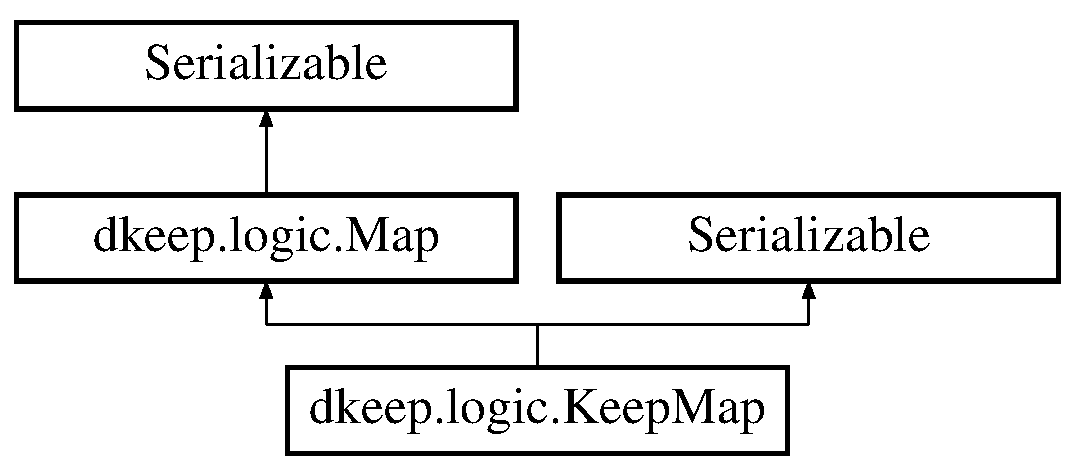
\includegraphics[height=3.000000cm]{classdkeep_1_1logic_1_1_keep_map}
\end{center}
\end{figure}
\subsection*{Public Member Functions}
\begin{DoxyCompactItemize}
\item 
\hyperlink{classdkeep_1_1logic_1_1_keep_map_a77443022f5af921bd511f4175a5adb6d}{Keep\+Map} ()
\item 
void \hyperlink{classdkeep_1_1logic_1_1_keep_map_a912c774ff749f78b0cf59509d0411a5c}{open\+Door} ()
\item 
\hyperlink{classdkeep_1_1logic_1_1_map}{Map} \hyperlink{classdkeep_1_1logic_1_1_keep_map_aee65a7c7233c2433140de2c97d989d4b}{next\+Map} ()
\end{DoxyCompactItemize}
\subsection*{Additional Inherited Members}


\subsection{Detailed Description}
Keepmap is a class that keeps information about the Keep map, containing the matrix of chars representing the map and it\textquotesingle{}s key. \begin{DoxySeeAlso}{See also}
\hyperlink{classdkeep_1_1logic_1_1_map}{Map} 
\end{DoxySeeAlso}


\subsection{Constructor \& Destructor Documentation}
\mbox{\Hypertarget{classdkeep_1_1logic_1_1_keep_map_a77443022f5af921bd511f4175a5adb6d}\label{classdkeep_1_1logic_1_1_keep_map_a77443022f5af921bd511f4175a5adb6d}} 
\index{dkeep\+::logic\+::\+Keep\+Map@{dkeep\+::logic\+::\+Keep\+Map}!Keep\+Map@{Keep\+Map}}
\index{Keep\+Map@{Keep\+Map}!dkeep\+::logic\+::\+Keep\+Map@{dkeep\+::logic\+::\+Keep\+Map}}
\subsubsection{\texorpdfstring{Keep\+Map()}{KeepMap()}}
{\footnotesize\ttfamily dkeep.\+logic.\+Keep\+Map.\+Keep\+Map (\begin{DoxyParamCaption}{ }\end{DoxyParamCaption})}

Constructor of \hyperlink{classdkeep_1_1logic_1_1_keep_map}{Keep\+Map}. Initializes the \hyperlink{classdkeep_1_1logic_1_1_map}{Map} attributes with the private attributes of this class. 

\subsection{Member Function Documentation}
\mbox{\Hypertarget{classdkeep_1_1logic_1_1_keep_map_aee65a7c7233c2433140de2c97d989d4b}\label{classdkeep_1_1logic_1_1_keep_map_aee65a7c7233c2433140de2c97d989d4b}} 
\index{dkeep\+::logic\+::\+Keep\+Map@{dkeep\+::logic\+::\+Keep\+Map}!next\+Map@{next\+Map}}
\index{next\+Map@{next\+Map}!dkeep\+::logic\+::\+Keep\+Map@{dkeep\+::logic\+::\+Keep\+Map}}
\subsubsection{\texorpdfstring{next\+Map()}{nextMap()}}
{\footnotesize\ttfamily \hyperlink{classdkeep_1_1logic_1_1_map}{Map} dkeep.\+logic.\+Keep\+Map.\+next\+Map (\begin{DoxyParamCaption}{ }\end{DoxyParamCaption})}

\mbox{\Hypertarget{classdkeep_1_1logic_1_1_keep_map_a912c774ff749f78b0cf59509d0411a5c}\label{classdkeep_1_1logic_1_1_keep_map_a912c774ff749f78b0cf59509d0411a5c}} 
\index{dkeep\+::logic\+::\+Keep\+Map@{dkeep\+::logic\+::\+Keep\+Map}!open\+Door@{open\+Door}}
\index{open\+Door@{open\+Door}!dkeep\+::logic\+::\+Keep\+Map@{dkeep\+::logic\+::\+Keep\+Map}}
\subsubsection{\texorpdfstring{open\+Door()}{openDoor()}}
{\footnotesize\ttfamily void dkeep.\+logic.\+Keep\+Map.\+open\+Door (\begin{DoxyParamCaption}{ }\end{DoxyParamCaption})}

In this particular class it doesn\textquotesingle{}t go through the map, it only opens the only door of the map. 

The documentation for this class was generated from the following file\+:\begin{DoxyCompactItemize}
\item 
C\+:/\+Users/\+M\+C-\/\+Guida/git/\+L\+P\+O\+O1617\+\_\+\+T1\+G5/\+Lab05/src/dkeep/logic/Keep\+Map.\+java\end{DoxyCompactItemize}

\hypertarget{classdkeep_1_1logic_1_1_logic}{}\section{dkeep.\+logic.\+Logic Class Reference}
\label{classdkeep_1_1logic_1_1_logic}\index{dkeep.\+logic.\+Logic@{dkeep.\+logic.\+Logic}}
Inheritance diagram for dkeep.\+logic.\+Logic\+:\begin{figure}[H]
\begin{center}
\leavevmode
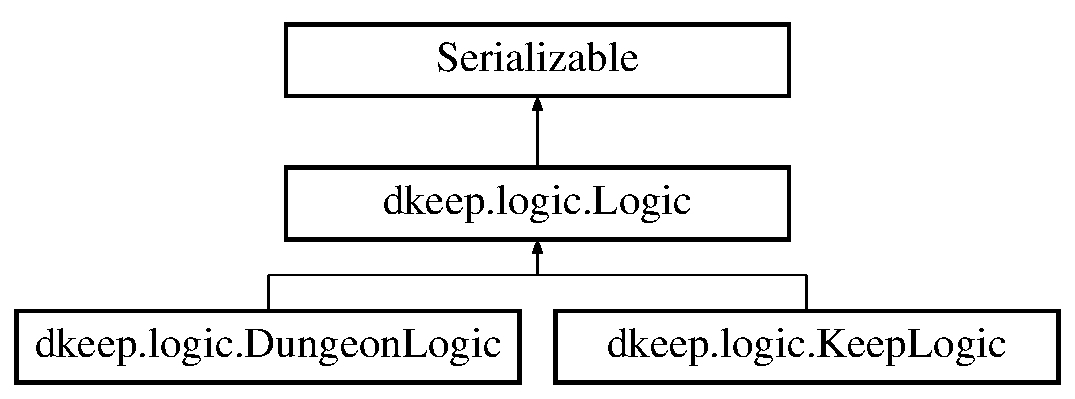
\includegraphics[height=3.000000cm]{classdkeep_1_1logic_1_1_logic}
\end{center}
\end{figure}
\subsection*{Public Member Functions}
\begin{DoxyCompactItemize}
\item 
\hyperlink{classdkeep_1_1logic_1_1_logic_a3e2a7548a462e06de5852e39df402b48}{Logic} (\hyperlink{classdkeep_1_1logic_1_1_hero}{Hero} hero)
\item 
void \hyperlink{classdkeep_1_1logic_1_1_logic_ad52a9235db954ca4014550582c94aa50}{add\+Enemy} (\hyperlink{classdkeep_1_1logic_1_1_character}{Character} enemy)
\item 
Array\+List$<$ \hyperlink{classdkeep_1_1logic_1_1_character}{Character} $>$ \hyperlink{classdkeep_1_1logic_1_1_logic_a2f36d0e37683459a9d26925b66842efb}{get\+Enemies} ()
\item 
\hyperlink{classdkeep_1_1logic_1_1_cell_position}{Cell\+Position} \hyperlink{classdkeep_1_1logic_1_1_logic_a83397013032b9ff9b023b52d54e2a839}{get\+Hero\+Position} ()
\item 
\hyperlink{classdkeep_1_1logic_1_1_hero}{Hero} \hyperlink{classdkeep_1_1logic_1_1_logic_a69dc81092b0395e64b0f09e6c39a355a}{get\+Hero} ()
\item 
char \hyperlink{classdkeep_1_1logic_1_1_logic_a8629375c65c00b778f7bc927ad30da72}{get\+Hero\+Symbol} ()
\item 
char \hyperlink{classdkeep_1_1logic_1_1_logic_a31914ab092089708b8b1a788a90b5bfc}{get\+Hero\+Weapon\+Symbol} ()
\item 
char \hyperlink{classdkeep_1_1logic_1_1_logic_aec99013c9c1b9e5a52615752e1e0a4f2}{get\+Enemy\+Symbol} ()
\item 
char \hyperlink{classdkeep_1_1logic_1_1_logic_a73d73f30185c2a55b7bc9d3e743dc6bf}{get\+Enemy\+Weapon\+Symbol} ()
\item 
boolean \hyperlink{classdkeep_1_1logic_1_1_logic_a4e216fa33c4ed8fc48649d6cac3e5b7a}{collide\+Left} (int\mbox{[}$\,$\mbox{]} pos1, int\mbox{[}$\,$\mbox{]} pos2)
\item 
boolean \hyperlink{classdkeep_1_1logic_1_1_logic_af55798f2e54446a1df0ebed4319f78bf}{collide\+Right} (int\mbox{[}$\,$\mbox{]} pos1, int\mbox{[}$\,$\mbox{]} pos2)
\item 
boolean \hyperlink{classdkeep_1_1logic_1_1_logic_af2fb54584f4206e935755e4bc5afce81}{collide\+Up} (int\mbox{[}$\,$\mbox{]} pos1, int\mbox{[}$\,$\mbox{]} pos2)
\item 
boolean \hyperlink{classdkeep_1_1logic_1_1_logic_a8918f9ee21260104e05bf39c43782e70}{collide\+Down} (int\mbox{[}$\,$\mbox{]} pos1, int\mbox{[}$\,$\mbox{]} pos2)
\item 
boolean \hyperlink{classdkeep_1_1logic_1_1_logic_aa038077e7e65bd2d047a125c5a7e6185}{collide\+Enemy} (int\mbox{[}$\,$\mbox{]} pos, Array\+List$<$ \hyperlink{classdkeep_1_1logic_1_1_character}{Character} $>$ vector)
\item 
boolean \hyperlink{classdkeep_1_1logic_1_1_logic_a6205c4d1912a64443bd9e5743d2db3bb}{collide\+Weapon} (int\mbox{[}$\,$\mbox{]} pos, Array\+List$<$ \hyperlink{classdkeep_1_1logic_1_1_weapon}{Weapon} $>$ vector)
\item 
void \hyperlink{classdkeep_1_1logic_1_1_logic_a6f9b5655e854e6460900b165f3f5f17a}{set\+Game\+Over} ()
\item 
Array\+List$<$ \hyperlink{classdkeep_1_1logic_1_1_weapon}{Weapon} $>$ \hyperlink{classdkeep_1_1logic_1_1_logic_af58982bc364016e2d0e03a36440a99b4}{get\+Weapons} ()
\item 
boolean \hyperlink{classdkeep_1_1logic_1_1_logic_a90069e7aa3f72919105ee446842e44fa}{move\+Hero} (char dir, \hyperlink{classdkeep_1_1logic_1_1_map}{Map} map)
\item 
void \hyperlink{classdkeep_1_1logic_1_1_logic_a1917b8f625dfb7c50ed2a2075209ed1a}{gameplay} (char dir, \hyperlink{classdkeep_1_1logic_1_1_map}{Map} map)
\item 
\hyperlink{classdkeep_1_1logic_1_1_logic}{Logic} \hyperlink{classdkeep_1_1logic_1_1_logic_a2f6e65021a7b525a5c61ebe1a56f09db}{next\+Logic} (\hyperlink{classdkeep_1_1logic_1_1_map}{Map} map, int option)
\item 
boolean \hyperlink{classdkeep_1_1logic_1_1_logic_a36229f271b0682f9a68c31390b4759cb}{game\+Over} ()
\item 
boolean \hyperlink{classdkeep_1_1logic_1_1_logic_a8873eb8f5bcdd55d87fe1e9953da00e0}{get\+Victory} ()
\end{DoxyCompactItemize}
\subsection*{Protected Attributes}
\begin{DoxyCompactItemize}
\item 
\mbox{\Hypertarget{classdkeep_1_1logic_1_1_logic_acf37fbec31325d4209c3127b9754b2e6}\label{classdkeep_1_1logic_1_1_logic_acf37fbec31325d4209c3127b9754b2e6}} 
\hyperlink{classdkeep_1_1logic_1_1_hero}{Hero} {\bfseries hero}
\item 
\mbox{\Hypertarget{classdkeep_1_1logic_1_1_logic_a2a25bee4f951f296f9cea3bb29f6ba07}\label{classdkeep_1_1logic_1_1_logic_a2a25bee4f951f296f9cea3bb29f6ba07}} 
Array\+List$<$ \hyperlink{classdkeep_1_1logic_1_1_character}{Character} $>$ {\bfseries enemies}
\item 
\mbox{\Hypertarget{classdkeep_1_1logic_1_1_logic_affc85b490b04c1b96994acfdfdcc1b50}\label{classdkeep_1_1logic_1_1_logic_affc85b490b04c1b96994acfdfdcc1b50}} 
boolean {\bfseries is\+Over}
\item 
\mbox{\Hypertarget{classdkeep_1_1logic_1_1_logic_a66c6502b38114e5af23068cb0089bbb2}\label{classdkeep_1_1logic_1_1_logic_a66c6502b38114e5af23068cb0089bbb2}} 
boolean {\bfseries victory}
\end{DoxyCompactItemize}


\subsection{Detailed Description}
\hyperlink{classdkeep_1_1logic_1_1_logic}{Logic} is a class that deals with all the logic of the current level of the game. It contains information about the current game elements, such as the hero, the enemies and a flag checks if the game is over and another that checks if it is a victory. It contains methods that deal with the movement of all the characters in the game and the collisions between them. 

\subsection{Constructor \& Destructor Documentation}
\mbox{\Hypertarget{classdkeep_1_1logic_1_1_logic_a3e2a7548a462e06de5852e39df402b48}\label{classdkeep_1_1logic_1_1_logic_a3e2a7548a462e06de5852e39df402b48}} 
\index{dkeep\+::logic\+::\+Logic@{dkeep\+::logic\+::\+Logic}!Logic@{Logic}}
\index{Logic@{Logic}!dkeep\+::logic\+::\+Logic@{dkeep\+::logic\+::\+Logic}}
\subsubsection{\texorpdfstring{Logic()}{Logic()}}
{\footnotesize\ttfamily dkeep.\+logic.\+Logic.\+Logic (\begin{DoxyParamCaption}\item[{\hyperlink{classdkeep_1_1logic_1_1_hero}{Hero}}]{hero }\end{DoxyParamCaption})}

Constructor of \hyperlink{classdkeep_1_1logic_1_1_logic}{Logic}. It initializes the hero with the variable given and puts all the flags to false. 
\begin{DoxyParams}{Parameters}
{\em hero} & Object \hyperlink{classdkeep_1_1logic_1_1_hero}{Hero} \\
\hline
\end{DoxyParams}


\subsection{Member Function Documentation}
\mbox{\Hypertarget{classdkeep_1_1logic_1_1_logic_ad52a9235db954ca4014550582c94aa50}\label{classdkeep_1_1logic_1_1_logic_ad52a9235db954ca4014550582c94aa50}} 
\index{dkeep\+::logic\+::\+Logic@{dkeep\+::logic\+::\+Logic}!add\+Enemy@{add\+Enemy}}
\index{add\+Enemy@{add\+Enemy}!dkeep\+::logic\+::\+Logic@{dkeep\+::logic\+::\+Logic}}
\subsubsection{\texorpdfstring{add\+Enemy()}{addEnemy()}}
{\footnotesize\ttfamily void dkeep.\+logic.\+Logic.\+add\+Enemy (\begin{DoxyParamCaption}\item[{\hyperlink{classdkeep_1_1logic_1_1_character}{Character}}]{enemy }\end{DoxyParamCaption})}

Adds an enemy to the arraylist of enemies 
\begin{DoxyParams}{Parameters}
{\em enemy} & Object \hyperlink{classdkeep_1_1logic_1_1_character}{Character} that represents an enemy \\
\hline
\end{DoxyParams}
\mbox{\Hypertarget{classdkeep_1_1logic_1_1_logic_a8918f9ee21260104e05bf39c43782e70}\label{classdkeep_1_1logic_1_1_logic_a8918f9ee21260104e05bf39c43782e70}} 
\index{dkeep\+::logic\+::\+Logic@{dkeep\+::logic\+::\+Logic}!collide\+Down@{collide\+Down}}
\index{collide\+Down@{collide\+Down}!dkeep\+::logic\+::\+Logic@{dkeep\+::logic\+::\+Logic}}
\subsubsection{\texorpdfstring{collide\+Down()}{collideDown()}}
{\footnotesize\ttfamily boolean dkeep.\+logic.\+Logic.\+collide\+Down (\begin{DoxyParamCaption}\item[{int \mbox{[}$\,$\mbox{]}}]{pos1,  }\item[{int \mbox{[}$\,$\mbox{]}}]{pos2 }\end{DoxyParamCaption})}

Checks if one of the elements is in the cell under the other element. If it is, it is a collision. 
\begin{DoxyParams}{Parameters}
{\em pos1} & array of ints with the position of an element of the game \\
\hline
{\em pos2} & array of ints with the position of an element of the game \\
\hline
\end{DoxyParams}
\begin{DoxyReturn}{Returns}
true if there is a collision, false if not 
\end{DoxyReturn}
\mbox{\Hypertarget{classdkeep_1_1logic_1_1_logic_aa038077e7e65bd2d047a125c5a7e6185}\label{classdkeep_1_1logic_1_1_logic_aa038077e7e65bd2d047a125c5a7e6185}} 
\index{dkeep\+::logic\+::\+Logic@{dkeep\+::logic\+::\+Logic}!collide\+Enemy@{collide\+Enemy}}
\index{collide\+Enemy@{collide\+Enemy}!dkeep\+::logic\+::\+Logic@{dkeep\+::logic\+::\+Logic}}
\subsubsection{\texorpdfstring{collide\+Enemy()}{collideEnemy()}}
{\footnotesize\ttfamily boolean dkeep.\+logic.\+Logic.\+collide\+Enemy (\begin{DoxyParamCaption}\item[{int \mbox{[}$\,$\mbox{]}}]{pos,  }\item[{Array\+List$<$ \hyperlink{classdkeep_1_1logic_1_1_character}{Character} $>$}]{vector }\end{DoxyParamCaption})}

Checks if the hero is in any position adjacent (up, down, left, right) to any of the enemies. If it is, it will return true, else it will return false. 
\begin{DoxyParams}{Parameters}
{\em x} & coordinate of the hero \\
\hline
{\em y} & coordinate of the hero \\
\hline
{\em vector} & contains all the enemies of the levels \\
\hline
\end{DoxyParams}
\begin{DoxyReturn}{Returns}
true if the hero collides with any of the enemies, false if it doesn\textquotesingle{}t 
\end{DoxyReturn}
\mbox{\Hypertarget{classdkeep_1_1logic_1_1_logic_a4e216fa33c4ed8fc48649d6cac3e5b7a}\label{classdkeep_1_1logic_1_1_logic_a4e216fa33c4ed8fc48649d6cac3e5b7a}} 
\index{dkeep\+::logic\+::\+Logic@{dkeep\+::logic\+::\+Logic}!collide\+Left@{collide\+Left}}
\index{collide\+Left@{collide\+Left}!dkeep\+::logic\+::\+Logic@{dkeep\+::logic\+::\+Logic}}
\subsubsection{\texorpdfstring{collide\+Left()}{collideLeft()}}
{\footnotesize\ttfamily boolean dkeep.\+logic.\+Logic.\+collide\+Left (\begin{DoxyParamCaption}\item[{int \mbox{[}$\,$\mbox{]}}]{pos1,  }\item[{int \mbox{[}$\,$\mbox{]}}]{pos2 }\end{DoxyParamCaption})}

Checks if one of the elements is in the cell to the left of the other element. If it is, it is a collision. 
\begin{DoxyParams}{Parameters}
{\em pos1} & array of ints with the position of an element of the game \\
\hline
{\em pos2} & array of ints with the position of an element of the game \\
\hline
\end{DoxyParams}
\begin{DoxyReturn}{Returns}
true if there is a collision, false if not 
\end{DoxyReturn}
\mbox{\Hypertarget{classdkeep_1_1logic_1_1_logic_af55798f2e54446a1df0ebed4319f78bf}\label{classdkeep_1_1logic_1_1_logic_af55798f2e54446a1df0ebed4319f78bf}} 
\index{dkeep\+::logic\+::\+Logic@{dkeep\+::logic\+::\+Logic}!collide\+Right@{collide\+Right}}
\index{collide\+Right@{collide\+Right}!dkeep\+::logic\+::\+Logic@{dkeep\+::logic\+::\+Logic}}
\subsubsection{\texorpdfstring{collide\+Right()}{collideRight()}}
{\footnotesize\ttfamily boolean dkeep.\+logic.\+Logic.\+collide\+Right (\begin{DoxyParamCaption}\item[{int \mbox{[}$\,$\mbox{]}}]{pos1,  }\item[{int \mbox{[}$\,$\mbox{]}}]{pos2 }\end{DoxyParamCaption})}

Checks if one of the elements is in the cell to the right of the other element. If it is, it is a collision. 
\begin{DoxyParams}{Parameters}
{\em pos1} & array of ints with the position of an element of the game \\
\hline
{\em pos2} & array of ints with the position of an element of the game \\
\hline
\end{DoxyParams}
\begin{DoxyReturn}{Returns}
true if there is a collision, false if not 
\end{DoxyReturn}
\mbox{\Hypertarget{classdkeep_1_1logic_1_1_logic_af2fb54584f4206e935755e4bc5afce81}\label{classdkeep_1_1logic_1_1_logic_af2fb54584f4206e935755e4bc5afce81}} 
\index{dkeep\+::logic\+::\+Logic@{dkeep\+::logic\+::\+Logic}!collide\+Up@{collide\+Up}}
\index{collide\+Up@{collide\+Up}!dkeep\+::logic\+::\+Logic@{dkeep\+::logic\+::\+Logic}}
\subsubsection{\texorpdfstring{collide\+Up()}{collideUp()}}
{\footnotesize\ttfamily boolean dkeep.\+logic.\+Logic.\+collide\+Up (\begin{DoxyParamCaption}\item[{int \mbox{[}$\,$\mbox{]}}]{pos1,  }\item[{int \mbox{[}$\,$\mbox{]}}]{pos2 }\end{DoxyParamCaption})}

Checks if one of the elements is in the cell above the other element. If it is, it is a collision. 
\begin{DoxyParams}{Parameters}
{\em pos1} & array of ints with the position of an element of the game \\
\hline
{\em pos2} & array of ints with the position of an element of the game \\
\hline
\end{DoxyParams}
\begin{DoxyReturn}{Returns}
true if there is a collision, false if not 
\end{DoxyReturn}
\mbox{\Hypertarget{classdkeep_1_1logic_1_1_logic_a6205c4d1912a64443bd9e5743d2db3bb}\label{classdkeep_1_1logic_1_1_logic_a6205c4d1912a64443bd9e5743d2db3bb}} 
\index{dkeep\+::logic\+::\+Logic@{dkeep\+::logic\+::\+Logic}!collide\+Weapon@{collide\+Weapon}}
\index{collide\+Weapon@{collide\+Weapon}!dkeep\+::logic\+::\+Logic@{dkeep\+::logic\+::\+Logic}}
\subsubsection{\texorpdfstring{collide\+Weapon()}{collideWeapon()}}
{\footnotesize\ttfamily boolean dkeep.\+logic.\+Logic.\+collide\+Weapon (\begin{DoxyParamCaption}\item[{int \mbox{[}$\,$\mbox{]}}]{pos,  }\item[{Array\+List$<$ \hyperlink{classdkeep_1_1logic_1_1_weapon}{Weapon} $>$}]{vector }\end{DoxyParamCaption})}

Checks if the \hyperlink{classdkeep_1_1logic_1_1_character}{Character} (can be both hero or enemy) is in any adjacent position to a weapon (can be from hero or enemy). If it is, it will return true, else false. 
\begin{DoxyParams}{Parameters}
{\em x} & coordinate of the \hyperlink{classdkeep_1_1logic_1_1_character}{Character} \\
\hline
{\em y} & coordinate of the \hyperlink{classdkeep_1_1logic_1_1_character}{Character} \\
\hline
{\em vector} & contains the weapons to be tested \\
\hline
\end{DoxyParams}
\begin{DoxyReturn}{Returns}
true if any of the weapons collide with the \hyperlink{classdkeep_1_1logic_1_1_character}{Character}, false id it doesn\textquotesingle{}t 
\end{DoxyReturn}
\mbox{\Hypertarget{classdkeep_1_1logic_1_1_logic_a36229f271b0682f9a68c31390b4759cb}\label{classdkeep_1_1logic_1_1_logic_a36229f271b0682f9a68c31390b4759cb}} 
\index{dkeep\+::logic\+::\+Logic@{dkeep\+::logic\+::\+Logic}!game\+Over@{game\+Over}}
\index{game\+Over@{game\+Over}!dkeep\+::logic\+::\+Logic@{dkeep\+::logic\+::\+Logic}}
\subsubsection{\texorpdfstring{game\+Over()}{gameOver()}}
{\footnotesize\ttfamily boolean dkeep.\+logic.\+Logic.\+game\+Over (\begin{DoxyParamCaption}{ }\end{DoxyParamCaption})}

Returns true if the game is over, false if it isn\textquotesingle{}t. \begin{DoxyReturn}{Returns}
true if the is\+Over is true, false if it isn\textquotesingle{}t 
\end{DoxyReturn}
\mbox{\Hypertarget{classdkeep_1_1logic_1_1_logic_a1917b8f625dfb7c50ed2a2075209ed1a}\label{classdkeep_1_1logic_1_1_logic_a1917b8f625dfb7c50ed2a2075209ed1a}} 
\index{dkeep\+::logic\+::\+Logic@{dkeep\+::logic\+::\+Logic}!gameplay@{gameplay}}
\index{gameplay@{gameplay}!dkeep\+::logic\+::\+Logic@{dkeep\+::logic\+::\+Logic}}
\subsubsection{\texorpdfstring{gameplay()}{gameplay()}}
{\footnotesize\ttfamily void dkeep.\+logic.\+Logic.\+gameplay (\begin{DoxyParamCaption}\item[{char}]{dir,  }\item[{\hyperlink{classdkeep_1_1logic_1_1_map}{Map}}]{map }\end{DoxyParamCaption})}

Handles all the movement logic of the game. It calls the functions that deal with the hero\textquotesingle{}s and hero\textquotesingle{}s weapon movement, and the enemies\textquotesingle{}s and enemies\textquotesingle{}s weapons movement. 
\begin{DoxyParams}{Parameters}
{\em dir} & char that correspond to the direction of the hero movement chosen by the player \\
\hline
{\em map} & Object \hyperlink{classdkeep_1_1logic_1_1_map}{Map} that corresponds to the current map of the game \\
\hline
\end{DoxyParams}
\mbox{\Hypertarget{classdkeep_1_1logic_1_1_logic_a2f36d0e37683459a9d26925b66842efb}\label{classdkeep_1_1logic_1_1_logic_a2f36d0e37683459a9d26925b66842efb}} 
\index{dkeep\+::logic\+::\+Logic@{dkeep\+::logic\+::\+Logic}!get\+Enemies@{get\+Enemies}}
\index{get\+Enemies@{get\+Enemies}!dkeep\+::logic\+::\+Logic@{dkeep\+::logic\+::\+Logic}}
\subsubsection{\texorpdfstring{get\+Enemies()}{getEnemies()}}
{\footnotesize\ttfamily Array\+List$<$\hyperlink{classdkeep_1_1logic_1_1_character}{Character}$>$ dkeep.\+logic.\+Logic.\+get\+Enemies (\begin{DoxyParamCaption}{ }\end{DoxyParamCaption})}

Return all the enemies that exist in the current level. \begin{DoxyReturn}{Returns}
Array\+List of Characters that correspond to the enemies of the level 
\end{DoxyReturn}
\mbox{\Hypertarget{classdkeep_1_1logic_1_1_logic_aec99013c9c1b9e5a52615752e1e0a4f2}\label{classdkeep_1_1logic_1_1_logic_aec99013c9c1b9e5a52615752e1e0a4f2}} 
\index{dkeep\+::logic\+::\+Logic@{dkeep\+::logic\+::\+Logic}!get\+Enemy\+Symbol@{get\+Enemy\+Symbol}}
\index{get\+Enemy\+Symbol@{get\+Enemy\+Symbol}!dkeep\+::logic\+::\+Logic@{dkeep\+::logic\+::\+Logic}}
\subsubsection{\texorpdfstring{get\+Enemy\+Symbol()}{getEnemySymbol()}}
{\footnotesize\ttfamily char dkeep.\+logic.\+Logic.\+get\+Enemy\+Symbol (\begin{DoxyParamCaption}{ }\end{DoxyParamCaption})}

Returns the symbol of the first enemy in the array of enemies. \begin{DoxyReturn}{Returns}
char that represents the enemy 
\end{DoxyReturn}
\mbox{\Hypertarget{classdkeep_1_1logic_1_1_logic_a73d73f30185c2a55b7bc9d3e743dc6bf}\label{classdkeep_1_1logic_1_1_logic_a73d73f30185c2a55b7bc9d3e743dc6bf}} 
\index{dkeep\+::logic\+::\+Logic@{dkeep\+::logic\+::\+Logic}!get\+Enemy\+Weapon\+Symbol@{get\+Enemy\+Weapon\+Symbol}}
\index{get\+Enemy\+Weapon\+Symbol@{get\+Enemy\+Weapon\+Symbol}!dkeep\+::logic\+::\+Logic@{dkeep\+::logic\+::\+Logic}}
\subsubsection{\texorpdfstring{get\+Enemy\+Weapon\+Symbol()}{getEnemyWeaponSymbol()}}
{\footnotesize\ttfamily char dkeep.\+logic.\+Logic.\+get\+Enemy\+Weapon\+Symbol (\begin{DoxyParamCaption}{ }\end{DoxyParamCaption})}

Returns the symbol of the first enemy\textquotesingle{}s weapon in the array of enemies. \begin{DoxyReturn}{Returns}
char that represents the enemy\textquotesingle{}s weapon 
\end{DoxyReturn}
\mbox{\Hypertarget{classdkeep_1_1logic_1_1_logic_a69dc81092b0395e64b0f09e6c39a355a}\label{classdkeep_1_1logic_1_1_logic_a69dc81092b0395e64b0f09e6c39a355a}} 
\index{dkeep\+::logic\+::\+Logic@{dkeep\+::logic\+::\+Logic}!get\+Hero@{get\+Hero}}
\index{get\+Hero@{get\+Hero}!dkeep\+::logic\+::\+Logic@{dkeep\+::logic\+::\+Logic}}
\subsubsection{\texorpdfstring{get\+Hero()}{getHero()}}
{\footnotesize\ttfamily \hyperlink{classdkeep_1_1logic_1_1_hero}{Hero} dkeep.\+logic.\+Logic.\+get\+Hero (\begin{DoxyParamCaption}{ }\end{DoxyParamCaption})}

Returns the hero. \begin{DoxyReturn}{Returns}
Object \hyperlink{classdkeep_1_1logic_1_1_hero}{Hero} 
\end{DoxyReturn}
\mbox{\Hypertarget{classdkeep_1_1logic_1_1_logic_a83397013032b9ff9b023b52d54e2a839}\label{classdkeep_1_1logic_1_1_logic_a83397013032b9ff9b023b52d54e2a839}} 
\index{dkeep\+::logic\+::\+Logic@{dkeep\+::logic\+::\+Logic}!get\+Hero\+Position@{get\+Hero\+Position}}
\index{get\+Hero\+Position@{get\+Hero\+Position}!dkeep\+::logic\+::\+Logic@{dkeep\+::logic\+::\+Logic}}
\subsubsection{\texorpdfstring{get\+Hero\+Position()}{getHeroPosition()}}
{\footnotesize\ttfamily \hyperlink{classdkeep_1_1logic_1_1_cell_position}{Cell\+Position} dkeep.\+logic.\+Logic.\+get\+Hero\+Position (\begin{DoxyParamCaption}{ }\end{DoxyParamCaption})}

Returns the \hyperlink{classdkeep_1_1logic_1_1_cell_position}{Cell\+Position} with the current coordinates of the hero. \begin{DoxyReturn}{Returns}
Object \hyperlink{classdkeep_1_1logic_1_1_cell_position}{Cell\+Position} that correspond to the position of the hero 
\end{DoxyReturn}
\mbox{\Hypertarget{classdkeep_1_1logic_1_1_logic_a8629375c65c00b778f7bc927ad30da72}\label{classdkeep_1_1logic_1_1_logic_a8629375c65c00b778f7bc927ad30da72}} 
\index{dkeep\+::logic\+::\+Logic@{dkeep\+::logic\+::\+Logic}!get\+Hero\+Symbol@{get\+Hero\+Symbol}}
\index{get\+Hero\+Symbol@{get\+Hero\+Symbol}!dkeep\+::logic\+::\+Logic@{dkeep\+::logic\+::\+Logic}}
\subsubsection{\texorpdfstring{get\+Hero\+Symbol()}{getHeroSymbol()}}
{\footnotesize\ttfamily char dkeep.\+logic.\+Logic.\+get\+Hero\+Symbol (\begin{DoxyParamCaption}{ }\end{DoxyParamCaption})}

Returns the symbol with which the hero is represented in the map. \begin{DoxyReturn}{Returns}
char that represents the hero 
\end{DoxyReturn}
\mbox{\Hypertarget{classdkeep_1_1logic_1_1_logic_a31914ab092089708b8b1a788a90b5bfc}\label{classdkeep_1_1logic_1_1_logic_a31914ab092089708b8b1a788a90b5bfc}} 
\index{dkeep\+::logic\+::\+Logic@{dkeep\+::logic\+::\+Logic}!get\+Hero\+Weapon\+Symbol@{get\+Hero\+Weapon\+Symbol}}
\index{get\+Hero\+Weapon\+Symbol@{get\+Hero\+Weapon\+Symbol}!dkeep\+::logic\+::\+Logic@{dkeep\+::logic\+::\+Logic}}
\subsubsection{\texorpdfstring{get\+Hero\+Weapon\+Symbol()}{getHeroWeaponSymbol()}}
{\footnotesize\ttfamily char dkeep.\+logic.\+Logic.\+get\+Hero\+Weapon\+Symbol (\begin{DoxyParamCaption}{ }\end{DoxyParamCaption})}

Returns the symbol with which the hero\textquotesingle{}s weapon is represented in the map. \begin{DoxyReturn}{Returns}
char that represents the hero\textquotesingle{}s weapon 
\end{DoxyReturn}
\mbox{\Hypertarget{classdkeep_1_1logic_1_1_logic_a8873eb8f5bcdd55d87fe1e9953da00e0}\label{classdkeep_1_1logic_1_1_logic_a8873eb8f5bcdd55d87fe1e9953da00e0}} 
\index{dkeep\+::logic\+::\+Logic@{dkeep\+::logic\+::\+Logic}!get\+Victory@{get\+Victory}}
\index{get\+Victory@{get\+Victory}!dkeep\+::logic\+::\+Logic@{dkeep\+::logic\+::\+Logic}}
\subsubsection{\texorpdfstring{get\+Victory()}{getVictory()}}
{\footnotesize\ttfamily boolean dkeep.\+logic.\+Logic.\+get\+Victory (\begin{DoxyParamCaption}{ }\end{DoxyParamCaption})}

Returns true if the player has won, false if it hasn\textquotesingle{}t. \begin{DoxyReturn}{Returns}
true if victory is true, false if it isn\textquotesingle{}t 
\end{DoxyReturn}
\mbox{\Hypertarget{classdkeep_1_1logic_1_1_logic_af58982bc364016e2d0e03a36440a99b4}\label{classdkeep_1_1logic_1_1_logic_af58982bc364016e2d0e03a36440a99b4}} 
\index{dkeep\+::logic\+::\+Logic@{dkeep\+::logic\+::\+Logic}!get\+Weapons@{get\+Weapons}}
\index{get\+Weapons@{get\+Weapons}!dkeep\+::logic\+::\+Logic@{dkeep\+::logic\+::\+Logic}}
\subsubsection{\texorpdfstring{get\+Weapons()}{getWeapons()}}
{\footnotesize\ttfamily Array\+List$<$\hyperlink{classdkeep_1_1logic_1_1_weapon}{Weapon}$>$ dkeep.\+logic.\+Logic.\+get\+Weapons (\begin{DoxyParamCaption}{ }\end{DoxyParamCaption})}

Goes through the enemies arraylist and groups their weapons into an arraylist, returning it. \begin{DoxyReturn}{Returns}
Array\+List with all the weapons of the enemies 
\end{DoxyReturn}
\mbox{\Hypertarget{classdkeep_1_1logic_1_1_logic_a90069e7aa3f72919105ee446842e44fa}\label{classdkeep_1_1logic_1_1_logic_a90069e7aa3f72919105ee446842e44fa}} 
\index{dkeep\+::logic\+::\+Logic@{dkeep\+::logic\+::\+Logic}!move\+Hero@{move\+Hero}}
\index{move\+Hero@{move\+Hero}!dkeep\+::logic\+::\+Logic@{dkeep\+::logic\+::\+Logic}}
\subsubsection{\texorpdfstring{move\+Hero()}{moveHero()}}
{\footnotesize\ttfamily boolean dkeep.\+logic.\+Logic.\+move\+Hero (\begin{DoxyParamCaption}\item[{char}]{dir,  }\item[{\hyperlink{classdkeep_1_1logic_1_1_map}{Map}}]{map }\end{DoxyParamCaption})}

Moves the hero accordingly to the dir variable, checking if it collides with the enemy (which makes the flag is\+Over to turn to true). It also checks if the direction chosen is a valid one, making sure it doesn\textquotesingle{}t overlap any of the static elements of the game. Furthermore, it also checks if the hero has caught the key or pulled the lever, using this information to change it\textquotesingle{}s behaviour once in front of doors. 
\begin{DoxyParams}{Parameters}
{\em dir} & char that correspond to the direction of movement chosen by the player \\
\hline
{\em map} & Object \hyperlink{classdkeep_1_1logic_1_1_map}{Map} that corresponds to the current map of the game \\
\hline
\end{DoxyParams}
\begin{DoxyReturn}{Returns}
true if the hero has made with no collisions, false if it was caught 
\end{DoxyReturn}
\mbox{\Hypertarget{classdkeep_1_1logic_1_1_logic_a2f6e65021a7b525a5c61ebe1a56f09db}\label{classdkeep_1_1logic_1_1_logic_a2f6e65021a7b525a5c61ebe1a56f09db}} 
\index{dkeep\+::logic\+::\+Logic@{dkeep\+::logic\+::\+Logic}!next\+Logic@{next\+Logic}}
\index{next\+Logic@{next\+Logic}!dkeep\+::logic\+::\+Logic@{dkeep\+::logic\+::\+Logic}}
\subsubsection{\texorpdfstring{next\+Logic()}{nextLogic()}}
{\footnotesize\ttfamily \hyperlink{classdkeep_1_1logic_1_1_logic}{Logic} dkeep.\+logic.\+Logic.\+next\+Logic (\begin{DoxyParamCaption}\item[{\hyperlink{classdkeep_1_1logic_1_1_map}{Map}}]{map,  }\item[{int}]{option }\end{DoxyParamCaption})}

Returns the logic of the next level. 
\begin{DoxyParams}{Parameters}
{\em map} & \hyperlink{classdkeep_1_1logic_1_1_map}{Map} of the next level \\
\hline
{\em option} & number or behaviour of the enemies of the next level \\
\hline
\end{DoxyParams}
\begin{DoxyReturn}{Returns}
\hyperlink{classdkeep_1_1logic_1_1_logic}{Logic} of the next level 
\end{DoxyReturn}
\mbox{\Hypertarget{classdkeep_1_1logic_1_1_logic_a6f9b5655e854e6460900b165f3f5f17a}\label{classdkeep_1_1logic_1_1_logic_a6f9b5655e854e6460900b165f3f5f17a}} 
\index{dkeep\+::logic\+::\+Logic@{dkeep\+::logic\+::\+Logic}!set\+Game\+Over@{set\+Game\+Over}}
\index{set\+Game\+Over@{set\+Game\+Over}!dkeep\+::logic\+::\+Logic@{dkeep\+::logic\+::\+Logic}}
\subsubsection{\texorpdfstring{set\+Game\+Over()}{setGameOver()}}
{\footnotesize\ttfamily void dkeep.\+logic.\+Logic.\+set\+Game\+Over (\begin{DoxyParamCaption}{ }\end{DoxyParamCaption})}

Puts the flag of the game over to true. 

The documentation for this class was generated from the following file\+:\begin{DoxyCompactItemize}
\item 
C\+:/\+Users/\+M\+C-\/\+Guida/git/\+L\+P\+O\+O1617\+\_\+\+T1\+G5/\+Lab05/src/dkeep/logic/Logic.\+java\end{DoxyCompactItemize}

\hypertarget{classdkeep_1_1logic_1_1_map}{}\section{dkeep.\+logic.\+Map Class Reference}
\label{classdkeep_1_1logic_1_1_map}\index{dkeep.\+logic.\+Map@{dkeep.\+logic.\+Map}}
Inheritance diagram for dkeep.\+logic.\+Map\+:\begin{figure}[H]
\begin{center}
\leavevmode
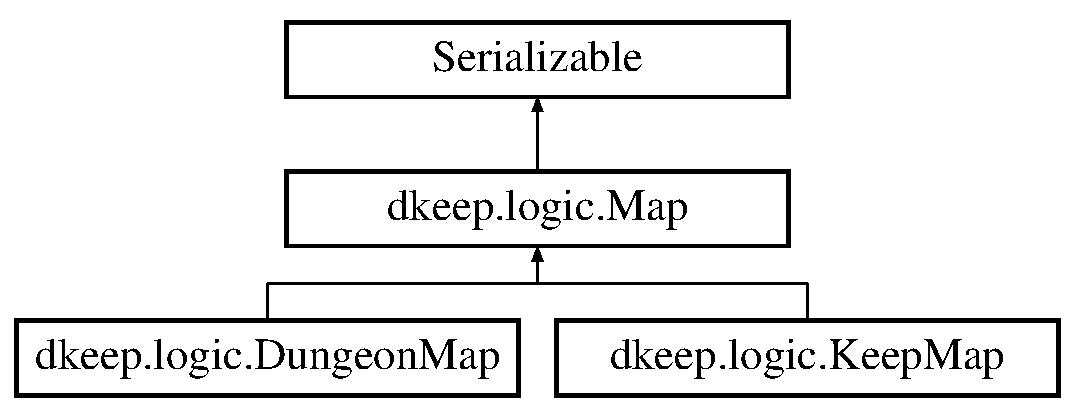
\includegraphics[height=3.000000cm]{classdkeep_1_1logic_1_1_map}
\end{center}
\end{figure}
\subsection*{Public Member Functions}
\begin{DoxyCompactItemize}
\item 
\hyperlink{classdkeep_1_1logic_1_1_map_a21bca3900428a3b8825b6da6214f2996}{Map} (char\mbox{[}$\,$\mbox{]}\mbox{[}$\,$\mbox{]} map, int\mbox{[}$\,$\mbox{]} key)
\item 
char \mbox{[}$\,$\mbox{]}\mbox{[}$\,$\mbox{]} \hyperlink{classdkeep_1_1logic_1_1_map_ab9624f3fa58049b3481f95e4c77277a3}{get\+Map} ()
\item 
void \hyperlink{classdkeep_1_1logic_1_1_map_af00c4221d9896abaa16dff00a462ba23}{set\+Map} (char\mbox{[}$\,$\mbox{]}\mbox{[}$\,$\mbox{]} map)
\item 
int \hyperlink{classdkeep_1_1logic_1_1_map_ad066c2de42a31b55a7649149cac143b2}{get\+Width} ()
\item 
int \hyperlink{classdkeep_1_1logic_1_1_map_aec82d7520e74ad90f897a34c30ebc056}{get\+Height} ()
\item 
int \mbox{[}$\,$\mbox{]} \hyperlink{classdkeep_1_1logic_1_1_map_aba4049e879891996457634979ec146a7}{get\+Key} ()
\item 
int \mbox{[}$\,$\mbox{]} \hyperlink{classdkeep_1_1logic_1_1_map_a94bbd79e68a9e0901cb129f9ef7bfa37}{get\+Hero\+Pos} ()
\item 
int \mbox{[}$\,$\mbox{]} \hyperlink{classdkeep_1_1logic_1_1_map_aeaad6dec94f54cf67dcb5c2bd23adbbf}{get\+Guard\+Pos} ()
\item 
int \mbox{[}$\,$\mbox{]} \hyperlink{classdkeep_1_1logic_1_1_map_a8dae121a32549da2035765a886f92d68}{get\+Ogre\+Pos} ()
\item 
void \hyperlink{classdkeep_1_1logic_1_1_map_a2d626ecdbda836f971f08ad31eadbd7b}{open\+Door} ()
\item 
boolean \hyperlink{classdkeep_1_1logic_1_1_map_a2237fa9a56d3aa3be8638be42bbc16e6}{are\+Doors\+Open} ()
\item 
boolean \hyperlink{classdkeep_1_1logic_1_1_map_a821f7fc33840cec683d9fe1d7146a3a5}{is\+Free} (int x, int y)
\item 
boolean \hyperlink{classdkeep_1_1logic_1_1_map_a721b87b71cb211ab754b9077963546f3}{is\+Key} (int x, int y)
\item 
boolean \hyperlink{classdkeep_1_1logic_1_1_map_a9af86cd24b6080738ca2059077249ff2}{isS} (int x, int y)
\item 
boolean \hyperlink{classdkeep_1_1logic_1_1_map_aa0e97d3c7fc51f4fa0caaa286745ff72}{isI} (int x, int y)
\item 
\hyperlink{classdkeep_1_1logic_1_1_map}{Map} \hyperlink{classdkeep_1_1logic_1_1_map_a05fd3c758bc198e790c9f04f2004bcb9}{next\+Map} ()
\end{DoxyCompactItemize}
\subsection*{Protected Attributes}
\begin{DoxyCompactItemize}
\item 
\mbox{\Hypertarget{classdkeep_1_1logic_1_1_map_a1233e77a9f52ff73c1e233790caba7f8}\label{classdkeep_1_1logic_1_1_map_a1233e77a9f52ff73c1e233790caba7f8}} 
char \mbox{[}$\,$\mbox{]}\mbox{[}$\,$\mbox{]} {\bfseries map}
\item 
\mbox{\Hypertarget{classdkeep_1_1logic_1_1_map_a38fbe49aa5250d71f3f0fb55c44ba973}\label{classdkeep_1_1logic_1_1_map_a38fbe49aa5250d71f3f0fb55c44ba973}} 
int \mbox{[}$\,$\mbox{]} {\bfseries key}
\end{DoxyCompactItemize}


\subsection{Detailed Description}
\hyperlink{classdkeep_1_1logic_1_1_map}{Map} is a class that keeps information about the map used in the game. It has a matrix of chars, used to store the map, and the position of it\textquotesingle{}s key. 

\subsection{Constructor \& Destructor Documentation}
\mbox{\Hypertarget{classdkeep_1_1logic_1_1_map_a21bca3900428a3b8825b6da6214f2996}\label{classdkeep_1_1logic_1_1_map_a21bca3900428a3b8825b6da6214f2996}} 
\index{dkeep\+::logic\+::\+Map@{dkeep\+::logic\+::\+Map}!Map@{Map}}
\index{Map@{Map}!dkeep\+::logic\+::\+Map@{dkeep\+::logic\+::\+Map}}
\subsubsection{\texorpdfstring{Map()}{Map()}}
{\footnotesize\ttfamily dkeep.\+logic.\+Map.\+Map (\begin{DoxyParamCaption}\item[{char}]{map\mbox{[}$\,$\mbox{]}\mbox{[}$\,$\mbox{]},  }\item[{int \mbox{[}$\,$\mbox{]}}]{key }\end{DoxyParamCaption})}

Constructor of \hyperlink{classdkeep_1_1logic_1_1_map}{Map}. It initializes its attributes with the values given. 
\begin{DoxyParams}{Parameters}
{\em map} & matrix of chars with the map setup \\
\hline
{\em key} & array of ints with the coordinates of the key in the map \\
\hline
\end{DoxyParams}


\subsection{Member Function Documentation}
\mbox{\Hypertarget{classdkeep_1_1logic_1_1_map_a2237fa9a56d3aa3be8638be42bbc16e6}\label{classdkeep_1_1logic_1_1_map_a2237fa9a56d3aa3be8638be42bbc16e6}} 
\index{dkeep\+::logic\+::\+Map@{dkeep\+::logic\+::\+Map}!are\+Doors\+Open@{are\+Doors\+Open}}
\index{are\+Doors\+Open@{are\+Doors\+Open}!dkeep\+::logic\+::\+Map@{dkeep\+::logic\+::\+Map}}
\subsubsection{\texorpdfstring{are\+Doors\+Open()}{areDoorsOpen()}}
{\footnotesize\ttfamily boolean dkeep.\+logic.\+Map.\+are\+Doors\+Open (\begin{DoxyParamCaption}{ }\end{DoxyParamCaption})}

Goes through the map and return true if it finds a open door. \begin{DoxyReturn}{Returns}
true if a door is open, false if it is not 
\end{DoxyReturn}
\mbox{\Hypertarget{classdkeep_1_1logic_1_1_map_aeaad6dec94f54cf67dcb5c2bd23adbbf}\label{classdkeep_1_1logic_1_1_map_aeaad6dec94f54cf67dcb5c2bd23adbbf}} 
\index{dkeep\+::logic\+::\+Map@{dkeep\+::logic\+::\+Map}!get\+Guard\+Pos@{get\+Guard\+Pos}}
\index{get\+Guard\+Pos@{get\+Guard\+Pos}!dkeep\+::logic\+::\+Map@{dkeep\+::logic\+::\+Map}}
\subsubsection{\texorpdfstring{get\+Guard\+Pos()}{getGuardPos()}}
{\footnotesize\ttfamily int \mbox{[}$\,$\mbox{]} dkeep.\+logic.\+Map.\+get\+Guard\+Pos (\begin{DoxyParamCaption}{ }\end{DoxyParamCaption})}

Goes through the map and coordinates of the enemy, returning them. Only works for Rookie\+Guards. \begin{DoxyReturn}{Returns}
array of ints with the actual coordinates of the guard 
\end{DoxyReturn}
\mbox{\Hypertarget{classdkeep_1_1logic_1_1_map_aec82d7520e74ad90f897a34c30ebc056}\label{classdkeep_1_1logic_1_1_map_aec82d7520e74ad90f897a34c30ebc056}} 
\index{dkeep\+::logic\+::\+Map@{dkeep\+::logic\+::\+Map}!get\+Height@{get\+Height}}
\index{get\+Height@{get\+Height}!dkeep\+::logic\+::\+Map@{dkeep\+::logic\+::\+Map}}
\subsubsection{\texorpdfstring{get\+Height()}{getHeight()}}
{\footnotesize\ttfamily int dkeep.\+logic.\+Map.\+get\+Height (\begin{DoxyParamCaption}{ }\end{DoxyParamCaption})}

Returns the map height. \begin{DoxyReturn}{Returns}
map height, which can also be called the maximum x coordinate -\/ 1 
\end{DoxyReturn}
\mbox{\Hypertarget{classdkeep_1_1logic_1_1_map_a94bbd79e68a9e0901cb129f9ef7bfa37}\label{classdkeep_1_1logic_1_1_map_a94bbd79e68a9e0901cb129f9ef7bfa37}} 
\index{dkeep\+::logic\+::\+Map@{dkeep\+::logic\+::\+Map}!get\+Hero\+Pos@{get\+Hero\+Pos}}
\index{get\+Hero\+Pos@{get\+Hero\+Pos}!dkeep\+::logic\+::\+Map@{dkeep\+::logic\+::\+Map}}
\subsubsection{\texorpdfstring{get\+Hero\+Pos()}{getHeroPos()}}
{\footnotesize\ttfamily int \mbox{[}$\,$\mbox{]} dkeep.\+logic.\+Map.\+get\+Hero\+Pos (\begin{DoxyParamCaption}{ }\end{DoxyParamCaption})}

Goes through the map and coordinates of the hero, returning them. \begin{DoxyReturn}{Returns}
array of ints with the actual coordinates of the hero 
\end{DoxyReturn}
\mbox{\Hypertarget{classdkeep_1_1logic_1_1_map_aba4049e879891996457634979ec146a7}\label{classdkeep_1_1logic_1_1_map_aba4049e879891996457634979ec146a7}} 
\index{dkeep\+::logic\+::\+Map@{dkeep\+::logic\+::\+Map}!get\+Key@{get\+Key}}
\index{get\+Key@{get\+Key}!dkeep\+::logic\+::\+Map@{dkeep\+::logic\+::\+Map}}
\subsubsection{\texorpdfstring{get\+Key()}{getKey()}}
{\footnotesize\ttfamily int \mbox{[}$\,$\mbox{]} dkeep.\+logic.\+Map.\+get\+Key (\begin{DoxyParamCaption}{ }\end{DoxyParamCaption})}

Returns the coordinates of the key. \begin{DoxyReturn}{Returns}
array of ints with the coordinates of the key in the map 
\end{DoxyReturn}
\mbox{\Hypertarget{classdkeep_1_1logic_1_1_map_ab9624f3fa58049b3481f95e4c77277a3}\label{classdkeep_1_1logic_1_1_map_ab9624f3fa58049b3481f95e4c77277a3}} 
\index{dkeep\+::logic\+::\+Map@{dkeep\+::logic\+::\+Map}!get\+Map@{get\+Map}}
\index{get\+Map@{get\+Map}!dkeep\+::logic\+::\+Map@{dkeep\+::logic\+::\+Map}}
\subsubsection{\texorpdfstring{get\+Map()}{getMap()}}
{\footnotesize\ttfamily char \mbox{[}$\,$\mbox{]}\mbox{[}$\,$\mbox{]} dkeep.\+logic.\+Map.\+get\+Map (\begin{DoxyParamCaption}{ }\end{DoxyParamCaption})}

Return a array of arrays that represent the map. \begin{DoxyReturn}{Returns}
array of array (matrix) of chars that represent the map 
\end{DoxyReturn}
\mbox{\Hypertarget{classdkeep_1_1logic_1_1_map_a8dae121a32549da2035765a886f92d68}\label{classdkeep_1_1logic_1_1_map_a8dae121a32549da2035765a886f92d68}} 
\index{dkeep\+::logic\+::\+Map@{dkeep\+::logic\+::\+Map}!get\+Ogre\+Pos@{get\+Ogre\+Pos}}
\index{get\+Ogre\+Pos@{get\+Ogre\+Pos}!dkeep\+::logic\+::\+Map@{dkeep\+::logic\+::\+Map}}
\subsubsection{\texorpdfstring{get\+Ogre\+Pos()}{getOgrePos()}}
{\footnotesize\ttfamily int \mbox{[}$\,$\mbox{]} dkeep.\+logic.\+Map.\+get\+Ogre\+Pos (\begin{DoxyParamCaption}{ }\end{DoxyParamCaption})}

Goes through the map and coordinates of the enemy, returning them. Only works for Crazy\+Ogres. \begin{DoxyReturn}{Returns}
array of ints with the actual coordinates of the ogre 
\end{DoxyReturn}
\mbox{\Hypertarget{classdkeep_1_1logic_1_1_map_ad066c2de42a31b55a7649149cac143b2}\label{classdkeep_1_1logic_1_1_map_ad066c2de42a31b55a7649149cac143b2}} 
\index{dkeep\+::logic\+::\+Map@{dkeep\+::logic\+::\+Map}!get\+Width@{get\+Width}}
\index{get\+Width@{get\+Width}!dkeep\+::logic\+::\+Map@{dkeep\+::logic\+::\+Map}}
\subsubsection{\texorpdfstring{get\+Width()}{getWidth()}}
{\footnotesize\ttfamily int dkeep.\+logic.\+Map.\+get\+Width (\begin{DoxyParamCaption}{ }\end{DoxyParamCaption})}

Returns the map width. \begin{DoxyReturn}{Returns}
map width, which can also be called the maximum y coordinate -\/ 1 
\end{DoxyReturn}
\mbox{\Hypertarget{classdkeep_1_1logic_1_1_map_a821f7fc33840cec683d9fe1d7146a3a5}\label{classdkeep_1_1logic_1_1_map_a821f7fc33840cec683d9fe1d7146a3a5}} 
\index{dkeep\+::logic\+::\+Map@{dkeep\+::logic\+::\+Map}!is\+Free@{is\+Free}}
\index{is\+Free@{is\+Free}!dkeep\+::logic\+::\+Map@{dkeep\+::logic\+::\+Map}}
\subsubsection{\texorpdfstring{is\+Free()}{isFree()}}
{\footnotesize\ttfamily boolean dkeep.\+logic.\+Map.\+is\+Free (\begin{DoxyParamCaption}\item[{int}]{x,  }\item[{int}]{y }\end{DoxyParamCaption})}

Checks if the cell with the coordinates given is free, meaning that in that position can\textquotesingle{}t be walls(\textquotesingle{}X\textquotesingle{}), closed and doors (\textquotesingle{}I\textquotesingle{},\textquotesingle{}S\textquotesingle{}). 
\begin{DoxyParams}{Parameters}
{\em x} & coordinate \\
\hline
{\em y} & coordinate \\
\hline
\end{DoxyParams}
\begin{DoxyReturn}{Returns}
true if position is free, false if it\textquotesingle{}s not 
\end{DoxyReturn}
\mbox{\Hypertarget{classdkeep_1_1logic_1_1_map_aa0e97d3c7fc51f4fa0caaa286745ff72}\label{classdkeep_1_1logic_1_1_map_aa0e97d3c7fc51f4fa0caaa286745ff72}} 
\index{dkeep\+::logic\+::\+Map@{dkeep\+::logic\+::\+Map}!isI@{isI}}
\index{isI@{isI}!dkeep\+::logic\+::\+Map@{dkeep\+::logic\+::\+Map}}
\subsubsection{\texorpdfstring{is\+I()}{isI()}}
{\footnotesize\ttfamily boolean dkeep.\+logic.\+Map.\+isI (\begin{DoxyParamCaption}\item[{int}]{x,  }\item[{int}]{y }\end{DoxyParamCaption})}

Checks if the given coordinates correspond to a closed door. 
\begin{DoxyParams}{Parameters}
{\em x} & coordinate \\
\hline
{\em y} & coordinate \\
\hline
\end{DoxyParams}
\begin{DoxyReturn}{Returns}
true if in the given coordinates is a closed door, false if it\textquotesingle{}s not 
\end{DoxyReturn}
\mbox{\Hypertarget{classdkeep_1_1logic_1_1_map_a721b87b71cb211ab754b9077963546f3}\label{classdkeep_1_1logic_1_1_map_a721b87b71cb211ab754b9077963546f3}} 
\index{dkeep\+::logic\+::\+Map@{dkeep\+::logic\+::\+Map}!is\+Key@{is\+Key}}
\index{is\+Key@{is\+Key}!dkeep\+::logic\+::\+Map@{dkeep\+::logic\+::\+Map}}
\subsubsection{\texorpdfstring{is\+Key()}{isKey()}}
{\footnotesize\ttfamily boolean dkeep.\+logic.\+Map.\+is\+Key (\begin{DoxyParamCaption}\item[{int}]{x,  }\item[{int}]{y }\end{DoxyParamCaption})}

Checks if the given coordinates match the position of the key. 
\begin{DoxyParams}{Parameters}
{\em x} & coordinate \\
\hline
{\em y} & coordinate \\
\hline
\end{DoxyParams}
\begin{DoxyReturn}{Returns}
true if the key is in given coordinates, false if it\textquotesingle{}s not 
\end{DoxyReturn}
\mbox{\Hypertarget{classdkeep_1_1logic_1_1_map_a9af86cd24b6080738ca2059077249ff2}\label{classdkeep_1_1logic_1_1_map_a9af86cd24b6080738ca2059077249ff2}} 
\index{dkeep\+::logic\+::\+Map@{dkeep\+::logic\+::\+Map}!isS@{isS}}
\index{isS@{isS}!dkeep\+::logic\+::\+Map@{dkeep\+::logic\+::\+Map}}
\subsubsection{\texorpdfstring{is\+S()}{isS()}}
{\footnotesize\ttfamily boolean dkeep.\+logic.\+Map.\+isS (\begin{DoxyParamCaption}\item[{int}]{x,  }\item[{int}]{y }\end{DoxyParamCaption})}

Checks if the given coordinates correspond to a open door. 
\begin{DoxyParams}{Parameters}
{\em x} & coordinate \\
\hline
{\em y} & coordinate \\
\hline
\end{DoxyParams}
\begin{DoxyReturn}{Returns}
true if in the given coordinates is a open door, false if it\textquotesingle{}s not 
\end{DoxyReturn}
\mbox{\Hypertarget{classdkeep_1_1logic_1_1_map_a05fd3c758bc198e790c9f04f2004bcb9}\label{classdkeep_1_1logic_1_1_map_a05fd3c758bc198e790c9f04f2004bcb9}} 
\index{dkeep\+::logic\+::\+Map@{dkeep\+::logic\+::\+Map}!next\+Map@{next\+Map}}
\index{next\+Map@{next\+Map}!dkeep\+::logic\+::\+Map@{dkeep\+::logic\+::\+Map}}
\subsubsection{\texorpdfstring{next\+Map()}{nextMap()}}
{\footnotesize\ttfamily \hyperlink{classdkeep_1_1logic_1_1_map}{Map} dkeep.\+logic.\+Map.\+next\+Map (\begin{DoxyParamCaption}{ }\end{DoxyParamCaption})}

Returns a new map if there is a next level, return null if there isn\textquotesingle{}t a next level. \begin{DoxyReturn}{Returns}
\hyperlink{classdkeep_1_1logic_1_1_map}{Map} or null 
\end{DoxyReturn}
\mbox{\Hypertarget{classdkeep_1_1logic_1_1_map_a2d626ecdbda836f971f08ad31eadbd7b}\label{classdkeep_1_1logic_1_1_map_a2d626ecdbda836f971f08ad31eadbd7b}} 
\index{dkeep\+::logic\+::\+Map@{dkeep\+::logic\+::\+Map}!open\+Door@{open\+Door}}
\index{open\+Door@{open\+Door}!dkeep\+::logic\+::\+Map@{dkeep\+::logic\+::\+Map}}
\subsubsection{\texorpdfstring{open\+Door()}{openDoor()}}
{\footnotesize\ttfamily void dkeep.\+logic.\+Map.\+open\+Door (\begin{DoxyParamCaption}{ }\end{DoxyParamCaption})}

Goes through the map, finding the chars representing the closed doors and switching them by chars representing the open doors. \mbox{\Hypertarget{classdkeep_1_1logic_1_1_map_af00c4221d9896abaa16dff00a462ba23}\label{classdkeep_1_1logic_1_1_map_af00c4221d9896abaa16dff00a462ba23}} 
\index{dkeep\+::logic\+::\+Map@{dkeep\+::logic\+::\+Map}!set\+Map@{set\+Map}}
\index{set\+Map@{set\+Map}!dkeep\+::logic\+::\+Map@{dkeep\+::logic\+::\+Map}}
\subsubsection{\texorpdfstring{set\+Map()}{setMap()}}
{\footnotesize\ttfamily void dkeep.\+logic.\+Map.\+set\+Map (\begin{DoxyParamCaption}\item[{char}]{map\mbox{[}$\,$\mbox{]}\mbox{[}$\,$\mbox{]} }\end{DoxyParamCaption})}

Sets the map attribute with the variable given. 
\begin{DoxyParams}{Parameters}
{\em map} & variable that represents the map to be updated \\
\hline
\end{DoxyParams}


The documentation for this class was generated from the following file\+:\begin{DoxyCompactItemize}
\item 
C\+:/\+Users/\+M\+C-\/\+Guida/git/\+L\+P\+O\+O1617\+\_\+\+T1\+G5/\+Lab05/src/dkeep/logic/Map.\+java\end{DoxyCompactItemize}

\hypertarget{classdkeep_1_1logic_1_1_rookie_guard}{}\section{dkeep.\+logic.\+Rookie\+Guard Class Reference}
\label{classdkeep_1_1logic_1_1_rookie_guard}\index{dkeep.\+logic.\+Rookie\+Guard@{dkeep.\+logic.\+Rookie\+Guard}}
Inheritance diagram for dkeep.\+logic.\+Rookie\+Guard\+:\begin{figure}[H]
\begin{center}
\leavevmode
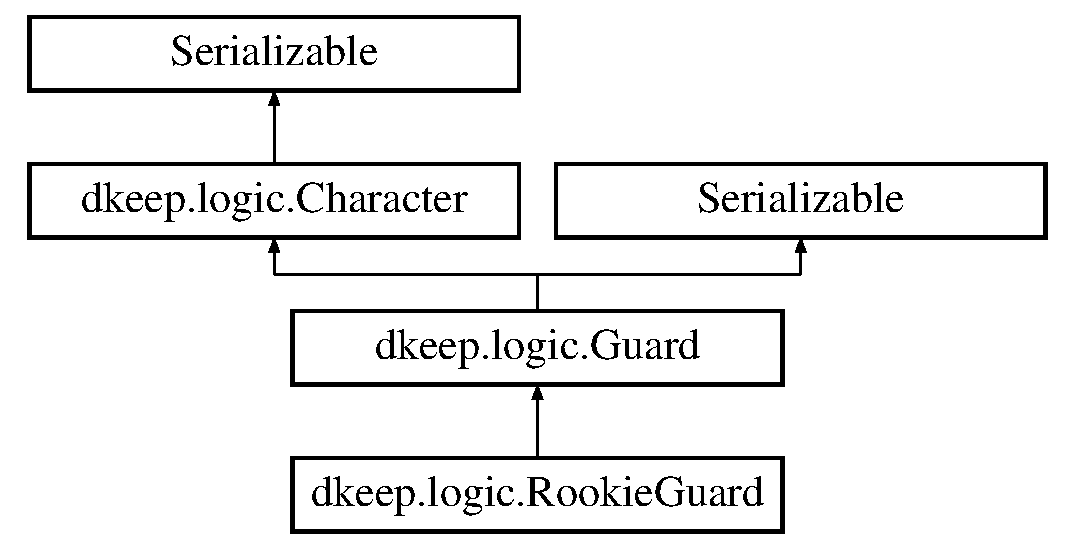
\includegraphics[height=4.000000cm]{classdkeep_1_1logic_1_1_rookie_guard}
\end{center}
\end{figure}
\subsection*{Public Member Functions}
\begin{DoxyCompactItemize}
\item 
\hyperlink{classdkeep_1_1logic_1_1_rookie_guard_ae9559d0efe10dbe17b8d923be52388ea}{Rookie\+Guard} (char symbol, int\mbox{[}$\,$\mbox{]} coord, char\mbox{[}$\,$\mbox{]} path)
\item 
int \mbox{[}$\,$\mbox{]} \hyperlink{classdkeep_1_1logic_1_1_rookie_guard_ae78bec3a34dbd5cbac6a90af92fd7984}{movement} ()
\item 
char \hyperlink{classdkeep_1_1logic_1_1_rookie_guard_a5e7a7811e8689941b19bd990d947bafd}{get\+Symbol} ()
\end{DoxyCompactItemize}
\subsection*{Additional Inherited Members}


\subsection{Detailed Description}
\hyperlink{classdkeep_1_1logic_1_1_rookie_guard}{Rookie\+Guard} is a class that contains information about the simplest of the guards. This guard merely follows the path given to him. \begin{DoxySeeAlso}{See also}
\hyperlink{classdkeep_1_1logic_1_1_guard}{Guard} 
\end{DoxySeeAlso}


\subsection{Constructor \& Destructor Documentation}
\mbox{\Hypertarget{classdkeep_1_1logic_1_1_rookie_guard_ae9559d0efe10dbe17b8d923be52388ea}\label{classdkeep_1_1logic_1_1_rookie_guard_ae9559d0efe10dbe17b8d923be52388ea}} 
\index{dkeep\+::logic\+::\+Rookie\+Guard@{dkeep\+::logic\+::\+Rookie\+Guard}!Rookie\+Guard@{Rookie\+Guard}}
\index{Rookie\+Guard@{Rookie\+Guard}!dkeep\+::logic\+::\+Rookie\+Guard@{dkeep\+::logic\+::\+Rookie\+Guard}}
\subsubsection{\texorpdfstring{Rookie\+Guard()}{RookieGuard()}}
{\footnotesize\ttfamily dkeep.\+logic.\+Rookie\+Guard.\+Rookie\+Guard (\begin{DoxyParamCaption}\item[{char}]{symbol,  }\item[{int \mbox{[}$\,$\mbox{]}}]{coord,  }\item[{char \mbox{[}$\,$\mbox{]}}]{path }\end{DoxyParamCaption})}

Constructor of the \hyperlink{classdkeep_1_1logic_1_1_rookie_guard}{Rookie\+Guard}. Puts the i variable to -\/1 and initializes other variables with the given values. 
\begin{DoxyParams}{Parameters}
{\em symbol} & char that represents the \hyperlink{classdkeep_1_1logic_1_1_rookie_guard}{Rookie\+Guard} \\
\hline
{\em x} & coordinate \\
\hline
{\em y} & coordinate \\
\hline
{\em path} & array of movements of the guard \\
\hline
\end{DoxyParams}


\subsection{Member Function Documentation}
\mbox{\Hypertarget{classdkeep_1_1logic_1_1_rookie_guard_a5e7a7811e8689941b19bd990d947bafd}\label{classdkeep_1_1logic_1_1_rookie_guard_a5e7a7811e8689941b19bd990d947bafd}} 
\index{dkeep\+::logic\+::\+Rookie\+Guard@{dkeep\+::logic\+::\+Rookie\+Guard}!get\+Symbol@{get\+Symbol}}
\index{get\+Symbol@{get\+Symbol}!dkeep\+::logic\+::\+Rookie\+Guard@{dkeep\+::logic\+::\+Rookie\+Guard}}
\subsubsection{\texorpdfstring{get\+Symbol()}{getSymbol()}}
{\footnotesize\ttfamily char dkeep.\+logic.\+Rookie\+Guard.\+get\+Symbol (\begin{DoxyParamCaption}{ }\end{DoxyParamCaption})}

\mbox{\Hypertarget{classdkeep_1_1logic_1_1_rookie_guard_ae78bec3a34dbd5cbac6a90af92fd7984}\label{classdkeep_1_1logic_1_1_rookie_guard_ae78bec3a34dbd5cbac6a90af92fd7984}} 
\index{dkeep\+::logic\+::\+Rookie\+Guard@{dkeep\+::logic\+::\+Rookie\+Guard}!movement@{movement}}
\index{movement@{movement}!dkeep\+::logic\+::\+Rookie\+Guard@{dkeep\+::logic\+::\+Rookie\+Guard}}
\subsubsection{\texorpdfstring{movement()}{movement()}}
{\footnotesize\ttfamily int \mbox{[}$\,$\mbox{]} dkeep.\+logic.\+Rookie\+Guard.\+movement (\begin{DoxyParamCaption}{ }\end{DoxyParamCaption})}

In this particular class, this function only calls the \hyperlink{classdkeep_1_1logic_1_1_guard_a2389016085c6d65d4366930fac72dab4}{normal\+Movement()} function, that follows the normal order of the path, and returns its output. 

The documentation for this class was generated from the following file\+:\begin{DoxyCompactItemize}
\item 
C\+:/\+Users/\+M\+C-\/\+Guida/git/\+L\+P\+O\+O1617\+\_\+\+T1\+G5/\+Lab05/src/dkeep/logic/Rookie\+Guard.\+java\end{DoxyCompactItemize}

\hypertarget{classdkeep_1_1logic_1_1_suspicious_guard}{}\section{dkeep.\+logic.\+Suspicious\+Guard Class Reference}
\label{classdkeep_1_1logic_1_1_suspicious_guard}\index{dkeep.\+logic.\+Suspicious\+Guard@{dkeep.\+logic.\+Suspicious\+Guard}}
Inheritance diagram for dkeep.\+logic.\+Suspicious\+Guard\+:\begin{figure}[H]
\begin{center}
\leavevmode
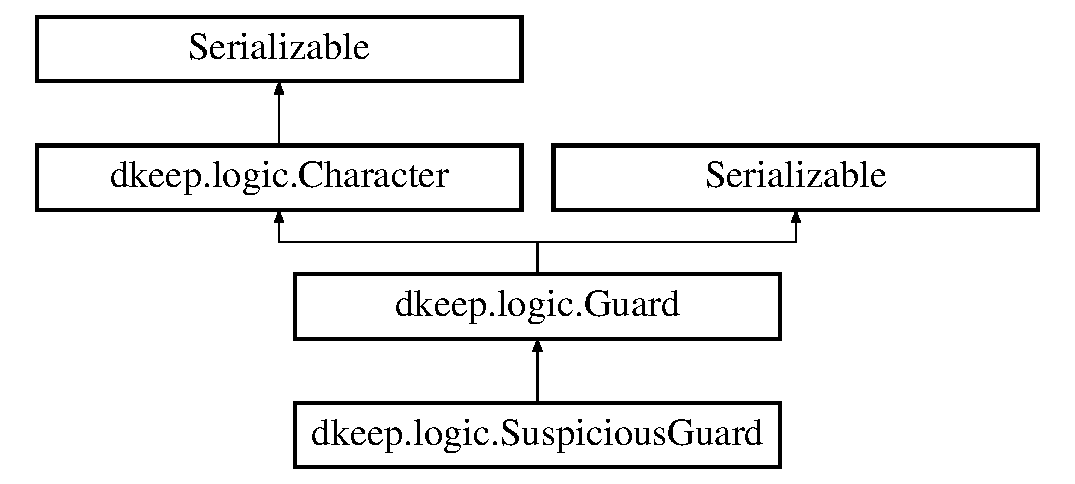
\includegraphics[height=4.000000cm]{classdkeep_1_1logic_1_1_suspicious_guard}
\end{center}
\end{figure}
\subsection*{Public Member Functions}
\begin{DoxyCompactItemize}
\item 
\hyperlink{classdkeep_1_1logic_1_1_suspicious_guard_a457daeb625091df0489c7a35598f6434}{Suspicious\+Guard} (char symbol, int\mbox{[}$\,$\mbox{]} coord, char\mbox{[}$\,$\mbox{]} path)
\item 
int \mbox{[}$\,$\mbox{]} \hyperlink{classdkeep_1_1logic_1_1_suspicious_guard_a10c4b42ec52624f5f4fbc8f38bb4faf1}{movement} ()
\item 
char \hyperlink{classdkeep_1_1logic_1_1_suspicious_guard_a760c8c915013dda755c4d0440071514f}{get\+Symbol} ()
\end{DoxyCompactItemize}
\subsection*{Additional Inherited Members}


\subsection{Detailed Description}
\hyperlink{classdkeep_1_1logic_1_1_suspicious_guard}{Suspicious\+Guard} is a class that contains information about a specific guard, which behaviour alternates between following the path in the normal order or in the reverse order. \begin{DoxySeeAlso}{See also}
\hyperlink{classdkeep_1_1logic_1_1_guard}{Guard} 
\end{DoxySeeAlso}


\subsection{Constructor \& Destructor Documentation}
\mbox{\Hypertarget{classdkeep_1_1logic_1_1_suspicious_guard_a457daeb625091df0489c7a35598f6434}\label{classdkeep_1_1logic_1_1_suspicious_guard_a457daeb625091df0489c7a35598f6434}} 
\index{dkeep\+::logic\+::\+Suspicious\+Guard@{dkeep\+::logic\+::\+Suspicious\+Guard}!Suspicious\+Guard@{Suspicious\+Guard}}
\index{Suspicious\+Guard@{Suspicious\+Guard}!dkeep\+::logic\+::\+Suspicious\+Guard@{dkeep\+::logic\+::\+Suspicious\+Guard}}
\subsubsection{\texorpdfstring{Suspicious\+Guard()}{SuspiciousGuard()}}
{\footnotesize\ttfamily dkeep.\+logic.\+Suspicious\+Guard.\+Suspicious\+Guard (\begin{DoxyParamCaption}\item[{char}]{symbol,  }\item[{int \mbox{[}$\,$\mbox{]}}]{coord,  }\item[{char \mbox{[}$\,$\mbox{]}}]{path }\end{DoxyParamCaption})}

Constructor of the \hyperlink{classdkeep_1_1logic_1_1_suspicious_guard}{Suspicious\+Guard}. Puts the i variable to -\/1 and initializes other variables with the given values, calling the \hyperlink{classdkeep_1_1logic_1_1_guard}{Guard} constructor. 
\begin{DoxyParams}{Parameters}
{\em symbol} & char that represents the \hyperlink{classdkeep_1_1logic_1_1_suspicious_guard}{Suspicious\+Guard} \\
\hline
{\em x} & coordinate \\
\hline
{\em y} & coordinate \\
\hline
{\em path} & array of movements of the guard \\
\hline
\end{DoxyParams}


\subsection{Member Function Documentation}
\mbox{\Hypertarget{classdkeep_1_1logic_1_1_suspicious_guard_a760c8c915013dda755c4d0440071514f}\label{classdkeep_1_1logic_1_1_suspicious_guard_a760c8c915013dda755c4d0440071514f}} 
\index{dkeep\+::logic\+::\+Suspicious\+Guard@{dkeep\+::logic\+::\+Suspicious\+Guard}!get\+Symbol@{get\+Symbol}}
\index{get\+Symbol@{get\+Symbol}!dkeep\+::logic\+::\+Suspicious\+Guard@{dkeep\+::logic\+::\+Suspicious\+Guard}}
\subsubsection{\texorpdfstring{get\+Symbol()}{getSymbol()}}
{\footnotesize\ttfamily char dkeep.\+logic.\+Suspicious\+Guard.\+get\+Symbol (\begin{DoxyParamCaption}{ }\end{DoxyParamCaption})}

\mbox{\Hypertarget{classdkeep_1_1logic_1_1_suspicious_guard_a10c4b42ec52624f5f4fbc8f38bb4faf1}\label{classdkeep_1_1logic_1_1_suspicious_guard_a10c4b42ec52624f5f4fbc8f38bb4faf1}} 
\index{dkeep\+::logic\+::\+Suspicious\+Guard@{dkeep\+::logic\+::\+Suspicious\+Guard}!movement@{movement}}
\index{movement@{movement}!dkeep\+::logic\+::\+Suspicious\+Guard@{dkeep\+::logic\+::\+Suspicious\+Guard}}
\subsubsection{\texorpdfstring{movement()}{movement()}}
{\footnotesize\ttfamily int \mbox{[}$\,$\mbox{]} dkeep.\+logic.\+Suspicious\+Guard.\+movement (\begin{DoxyParamCaption}{ }\end{DoxyParamCaption})}

in this particular class, this function randomly chooses between 2 behaviours, the normal one (follows the path and calls the \hyperlink{classdkeep_1_1logic_1_1_guard_a2389016085c6d65d4366930fac72dab4}{normal\+Movement()} function) and the reverse one (follows the path in reverse order, calls the \hyperlink{classdkeep_1_1logic_1_1_guard_a8c588aa887fcfe6d3e4a9e13d236c644}{reverse\+Movement()} function). 

The documentation for this class was generated from the following file\+:\begin{DoxyCompactItemize}
\item 
C\+:/\+Users/\+M\+C-\/\+Guida/git/\+L\+P\+O\+O1617\+\_\+\+T1\+G5/\+Lab05/src/dkeep/logic/Suspicious\+Guard.\+java\end{DoxyCompactItemize}

\hypertarget{classdkeep_1_1logic_1_1_weapon}{}\section{dkeep.\+logic.\+Weapon Class Reference}
\label{classdkeep_1_1logic_1_1_weapon}\index{dkeep.\+logic.\+Weapon@{dkeep.\+logic.\+Weapon}}
Inheritance diagram for dkeep.\+logic.\+Weapon\+:\begin{figure}[H]
\begin{center}
\leavevmode
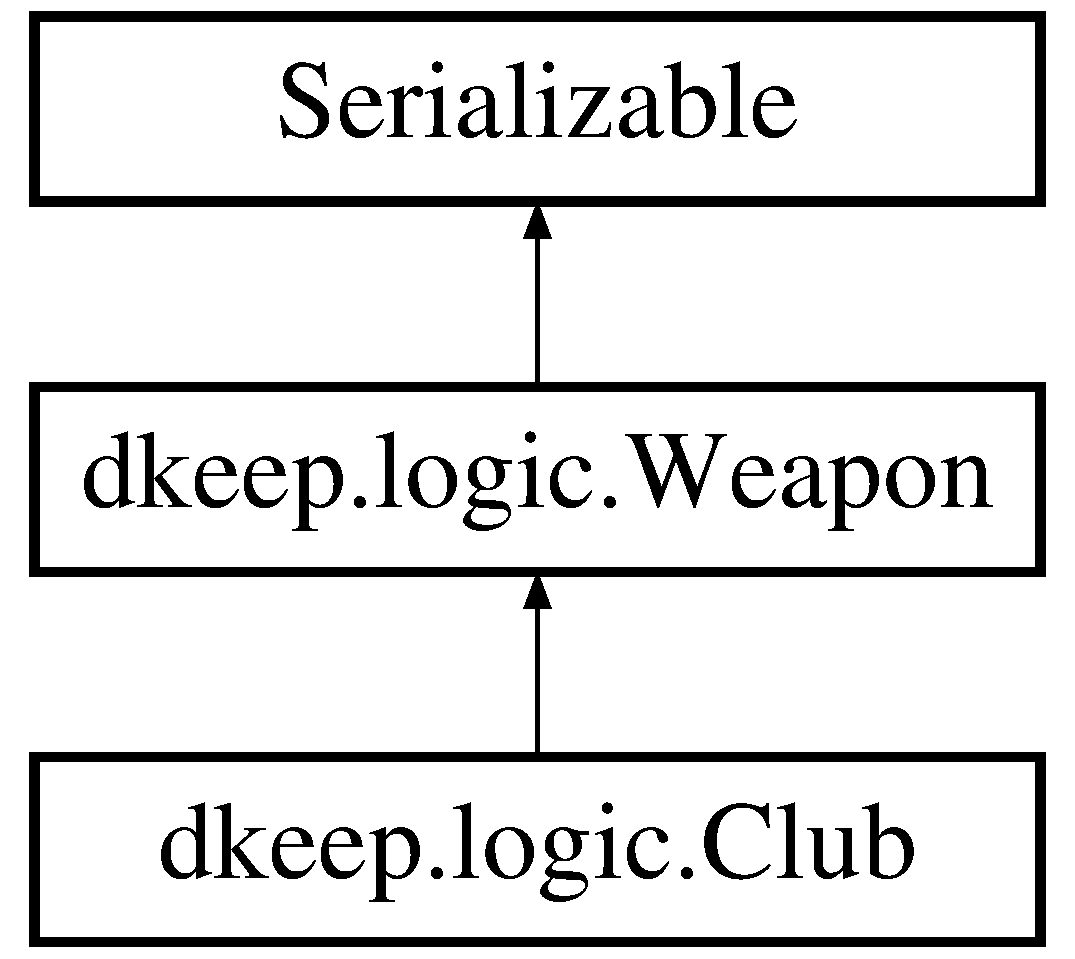
\includegraphics[height=3.000000cm]{classdkeep_1_1logic_1_1_weapon}
\end{center}
\end{figure}
\subsection*{Public Member Functions}
\begin{DoxyCompactItemize}
\item 
abstract int \mbox{[}$\,$\mbox{]} \hyperlink{classdkeep_1_1logic_1_1_weapon_adb73dd1c376c37614cad2b5ad2e9d1d4}{swing} (int x, int y)
\item 
int \hyperlink{classdkeep_1_1logic_1_1_weapon_a91b3f16c06cb271d31f1aa013c45ce31}{getX} ()
\item 
int \hyperlink{classdkeep_1_1logic_1_1_weapon_a5e47ccc0670cc36854af2dd1f72a70ee}{getY} ()
\item 
void \hyperlink{classdkeep_1_1logic_1_1_weapon_a5be1b0ffe5c917345fad810d83307461}{setX} (int x)
\item 
void \hyperlink{classdkeep_1_1logic_1_1_weapon_a11572cdd07ba03705550964e1d076e9c}{setY} (int y)
\item 
void \hyperlink{classdkeep_1_1logic_1_1_weapon_a93d2e4eb12cf90e2f07d54e7f99e2446}{set\+Not\+Valid} ()
\item 
void \hyperlink{classdkeep_1_1logic_1_1_weapon_a73776355a004878e7ca9a0a32033426f}{set\+Valid} ()
\item 
boolean \hyperlink{classdkeep_1_1logic_1_1_weapon_a68d3c9c406b56366ccfd75cae899bb68}{get\+Valid} ()
\item 
char \hyperlink{classdkeep_1_1logic_1_1_weapon_ad60afd31631a1552c749b5ddd0a5b949}{get\+Symbol} ()
\end{DoxyCompactItemize}
\subsection*{Protected Attributes}
\begin{DoxyCompactItemize}
\item 
\mbox{\Hypertarget{classdkeep_1_1logic_1_1_weapon_af6f8a376f3f843d84890f823b696449d}\label{classdkeep_1_1logic_1_1_weapon_af6f8a376f3f843d84890f823b696449d}} 
int {\bfseries x}
\item 
\mbox{\Hypertarget{classdkeep_1_1logic_1_1_weapon_adab0e9dd2253065c9bf26eb90df44937}\label{classdkeep_1_1logic_1_1_weapon_adab0e9dd2253065c9bf26eb90df44937}} 
int {\bfseries y}
\item 
\mbox{\Hypertarget{classdkeep_1_1logic_1_1_weapon_ac25e811e29333780f6f1ddf88b22c202}\label{classdkeep_1_1logic_1_1_weapon_ac25e811e29333780f6f1ddf88b22c202}} 
char {\bfseries symbol}
\item 
\mbox{\Hypertarget{classdkeep_1_1logic_1_1_weapon_a676b1b620341ad36649cd8408475c56b}\label{classdkeep_1_1logic_1_1_weapon_a676b1b620341ad36649cd8408475c56b}} 
char {\bfseries secsymbol}
\item 
\mbox{\Hypertarget{classdkeep_1_1logic_1_1_weapon_a89d4f4b0d4c737af7ef786e88f254085}\label{classdkeep_1_1logic_1_1_weapon_a89d4f4b0d4c737af7ef786e88f254085}} 
boolean {\bfseries above}
\item 
\mbox{\Hypertarget{classdkeep_1_1logic_1_1_weapon_a453cf282b3402e717715f3f3c6154a67}\label{classdkeep_1_1logic_1_1_weapon_a453cf282b3402e717715f3f3c6154a67}} 
boolean {\bfseries valid}
\end{DoxyCompactItemize}


\subsection{Detailed Description}
\hyperlink{classdkeep_1_1logic_1_1_weapon}{Weapon} is a class that represents a weapon possessed by a character. It keeps information about it\textquotesingle{}s symbols, coordinates, and flags informing if it\textquotesingle{}s position is above key and if it is in a vlid position to be printed. 

\subsection{Member Function Documentation}
\mbox{\Hypertarget{classdkeep_1_1logic_1_1_weapon_ad60afd31631a1552c749b5ddd0a5b949}\label{classdkeep_1_1logic_1_1_weapon_ad60afd31631a1552c749b5ddd0a5b949}} 
\index{dkeep\+::logic\+::\+Weapon@{dkeep\+::logic\+::\+Weapon}!get\+Symbol@{get\+Symbol}}
\index{get\+Symbol@{get\+Symbol}!dkeep\+::logic\+::\+Weapon@{dkeep\+::logic\+::\+Weapon}}
\subsubsection{\texorpdfstring{get\+Symbol()}{getSymbol()}}
{\footnotesize\ttfamily char dkeep.\+logic.\+Weapon.\+get\+Symbol (\begin{DoxyParamCaption}{ }\end{DoxyParamCaption})}

Returns the char representing the weapon based on it\textquotesingle{}s status. \begin{DoxyReturn}{Returns}
char representing the weapon 
\end{DoxyReturn}
\mbox{\Hypertarget{classdkeep_1_1logic_1_1_weapon_a68d3c9c406b56366ccfd75cae899bb68}\label{classdkeep_1_1logic_1_1_weapon_a68d3c9c406b56366ccfd75cae899bb68}} 
\index{dkeep\+::logic\+::\+Weapon@{dkeep\+::logic\+::\+Weapon}!get\+Valid@{get\+Valid}}
\index{get\+Valid@{get\+Valid}!dkeep\+::logic\+::\+Weapon@{dkeep\+::logic\+::\+Weapon}}
\subsubsection{\texorpdfstring{get\+Valid()}{getValid()}}
{\footnotesize\ttfamily boolean dkeep.\+logic.\+Weapon.\+get\+Valid (\begin{DoxyParamCaption}{ }\end{DoxyParamCaption})}

Returns the value of the flag valid. \begin{DoxyReturn}{Returns}
true if valid is true, false if valid is false 
\end{DoxyReturn}
\mbox{\Hypertarget{classdkeep_1_1logic_1_1_weapon_a91b3f16c06cb271d31f1aa013c45ce31}\label{classdkeep_1_1logic_1_1_weapon_a91b3f16c06cb271d31f1aa013c45ce31}} 
\index{dkeep\+::logic\+::\+Weapon@{dkeep\+::logic\+::\+Weapon}!getX@{getX}}
\index{getX@{getX}!dkeep\+::logic\+::\+Weapon@{dkeep\+::logic\+::\+Weapon}}
\subsubsection{\texorpdfstring{get\+X()}{getX()}}
{\footnotesize\ttfamily int dkeep.\+logic.\+Weapon.\+getX (\begin{DoxyParamCaption}{ }\end{DoxyParamCaption})}

Retrieve the valor of the coordinate x. \begin{DoxyReturn}{Returns}
the coordinate x, type int 
\end{DoxyReturn}
\mbox{\Hypertarget{classdkeep_1_1logic_1_1_weapon_a5e47ccc0670cc36854af2dd1f72a70ee}\label{classdkeep_1_1logic_1_1_weapon_a5e47ccc0670cc36854af2dd1f72a70ee}} 
\index{dkeep\+::logic\+::\+Weapon@{dkeep\+::logic\+::\+Weapon}!getY@{getY}}
\index{getY@{getY}!dkeep\+::logic\+::\+Weapon@{dkeep\+::logic\+::\+Weapon}}
\subsubsection{\texorpdfstring{get\+Y()}{getY()}}
{\footnotesize\ttfamily int dkeep.\+logic.\+Weapon.\+getY (\begin{DoxyParamCaption}{ }\end{DoxyParamCaption})}

Retrieve the valor of the coordinate y. \begin{DoxyReturn}{Returns}
the coordinate y, type int 
\end{DoxyReturn}
\mbox{\Hypertarget{classdkeep_1_1logic_1_1_weapon_a93d2e4eb12cf90e2f07d54e7f99e2446}\label{classdkeep_1_1logic_1_1_weapon_a93d2e4eb12cf90e2f07d54e7f99e2446}} 
\index{dkeep\+::logic\+::\+Weapon@{dkeep\+::logic\+::\+Weapon}!set\+Not\+Valid@{set\+Not\+Valid}}
\index{set\+Not\+Valid@{set\+Not\+Valid}!dkeep\+::logic\+::\+Weapon@{dkeep\+::logic\+::\+Weapon}}
\subsubsection{\texorpdfstring{set\+Not\+Valid()}{setNotValid()}}
{\footnotesize\ttfamily void dkeep.\+logic.\+Weapon.\+set\+Not\+Valid (\begin{DoxyParamCaption}{ }\end{DoxyParamCaption})}

Sets the valid flag to false, meaning that the weapon is in a position not valid to be printed. \mbox{\Hypertarget{classdkeep_1_1logic_1_1_weapon_a73776355a004878e7ca9a0a32033426f}\label{classdkeep_1_1logic_1_1_weapon_a73776355a004878e7ca9a0a32033426f}} 
\index{dkeep\+::logic\+::\+Weapon@{dkeep\+::logic\+::\+Weapon}!set\+Valid@{set\+Valid}}
\index{set\+Valid@{set\+Valid}!dkeep\+::logic\+::\+Weapon@{dkeep\+::logic\+::\+Weapon}}
\subsubsection{\texorpdfstring{set\+Valid()}{setValid()}}
{\footnotesize\ttfamily void dkeep.\+logic.\+Weapon.\+set\+Valid (\begin{DoxyParamCaption}{ }\end{DoxyParamCaption})}

Sets the valid flag to true, meaning that the weapon is in a position valid to be printed. \mbox{\Hypertarget{classdkeep_1_1logic_1_1_weapon_a5be1b0ffe5c917345fad810d83307461}\label{classdkeep_1_1logic_1_1_weapon_a5be1b0ffe5c917345fad810d83307461}} 
\index{dkeep\+::logic\+::\+Weapon@{dkeep\+::logic\+::\+Weapon}!setX@{setX}}
\index{setX@{setX}!dkeep\+::logic\+::\+Weapon@{dkeep\+::logic\+::\+Weapon}}
\subsubsection{\texorpdfstring{set\+X()}{setX()}}
{\footnotesize\ttfamily void dkeep.\+logic.\+Weapon.\+setX (\begin{DoxyParamCaption}\item[{int}]{x }\end{DoxyParamCaption})}

Set the coordinate x to the value given. 
\begin{DoxyParams}{Parameters}
{\em x} & new coordinate to be updated \\
\hline
\end{DoxyParams}
\mbox{\Hypertarget{classdkeep_1_1logic_1_1_weapon_a11572cdd07ba03705550964e1d076e9c}\label{classdkeep_1_1logic_1_1_weapon_a11572cdd07ba03705550964e1d076e9c}} 
\index{dkeep\+::logic\+::\+Weapon@{dkeep\+::logic\+::\+Weapon}!setY@{setY}}
\index{setY@{setY}!dkeep\+::logic\+::\+Weapon@{dkeep\+::logic\+::\+Weapon}}
\subsubsection{\texorpdfstring{set\+Y()}{setY()}}
{\footnotesize\ttfamily void dkeep.\+logic.\+Weapon.\+setY (\begin{DoxyParamCaption}\item[{int}]{y }\end{DoxyParamCaption})}

Set the coordinate y to the value given. 
\begin{DoxyParams}{Parameters}
{\em y} & new coordinate to be updated \\
\hline
\end{DoxyParams}
\mbox{\Hypertarget{classdkeep_1_1logic_1_1_weapon_adb73dd1c376c37614cad2b5ad2e9d1d4}\label{classdkeep_1_1logic_1_1_weapon_adb73dd1c376c37614cad2b5ad2e9d1d4}} 
\index{dkeep\+::logic\+::\+Weapon@{dkeep\+::logic\+::\+Weapon}!swing@{swing}}
\index{swing@{swing}!dkeep\+::logic\+::\+Weapon@{dkeep\+::logic\+::\+Weapon}}
\subsubsection{\texorpdfstring{swing()}{swing()}}
{\footnotesize\ttfamily abstract int \mbox{[}$\,$\mbox{]} dkeep.\+logic.\+Weapon.\+swing (\begin{DoxyParamCaption}\item[{int}]{x,  }\item[{int}]{y }\end{DoxyParamCaption})\hspace{0.3cm}{\ttfamily [abstract]}}

Using the coordinates of the weapon\textquotesingle{}s character (x and y), randomly calculates the direction of the next position of the weapon, returning a array of ints that represent the new coordinates for the weapon to take. 
\begin{DoxyParams}{Parameters}
{\em x} & coordinates of the weapon\textquotesingle{}s \hyperlink{classdkeep_1_1logic_1_1_character}{Character} \\
\hline
{\em y} & coordinates of the weapon\textquotesingle{}s \hyperlink{classdkeep_1_1logic_1_1_character}{Character} \\
\hline
\end{DoxyParams}
\begin{DoxyReturn}{Returns}
array of ints with coordinates x and y 
\end{DoxyReturn}


The documentation for this class was generated from the following file\+:\begin{DoxyCompactItemize}
\item 
C\+:/\+Users/\+M\+C-\/\+Guida/git/\+L\+P\+O\+O1617\+\_\+\+T1\+G5/\+Lab05/src/dkeep/logic/Weapon.\+java\end{DoxyCompactItemize}

%--- End generated contents ---

% Index
\backmatter
\newpage
\phantomsection
\clearemptydoublepage
\addcontentsline{toc}{chapter}{Index}
\printindex

\end{document}
